
\typeout{new file: Verification_Tests_Chapter.tex}

\chapter{Verification Tests}
\label{sec:verification}

This chapter reports the results of the verification tests performed with the new fuel data, \textit{i.e.} Ethylene ($\rm C_2H_4$), Ethane ($\rm C_2H_6$), Propylene ($\rm C_3H_6$), Propane ($\rm C_3H_8$), Toluene ($\rm C_7H_8$),
  \textit{n}-Heptane ($\rm C_7H_{16}$), Methanol ($\rm CH_3OH$), Methyl Methacrylate ($\rm C_5H_8O_2$). Synthetic transmissivity spectrum were generated with RadCal and compared with all the experimental data they were extract from. The experimental data resolution was adjusted to match that of RadCal:
\begin{equation}
 \begin{cases}
   5~{\rm cm}^{-1},\, & \om \leq 1000 {\rm cm^{-1}}\\
    25~{\rm cm}^{-1},\,& 5000 > \om > 1000 {\rm cm^{-1}} \\
    50~{\rm cm}^{-1},\,& \om > 5000 {\rm cm^{-1}}
 \end{cases}
\end{equation}

The relative error between the experimental and the RadCal-generated transmissivity, denoted $\epsilon{(\tau_{\omega})}$, was also quantified. The relative error between the experimental and the RadCal calculated transmissivities can also be quantified by a weighted average relative error $\epsilon$ over the entire experimental spectrum. A useful test function to perform the weighting is given by the spectral emissivity. Assuming Kirchhoff's law applies for each wavenumber over a narrow band, the spectral emissivity of a narrow band, denoted $\bar{\varepsilon}_{\omega}$, is given by:
\begin{equation}
 \bar{\varepsilon}_{\omega} = 1 -\bar{\tau}_{\omega}.
\end{equation}
The weighted average error is then defined by the following relation:
\begin{equation}
\label{eq:WeightedError}
 \langle\epsilon{(\bar{\tau}_{\omega})}\rangle = \dfrac{\displaystyle\int\limits_{700}^{4000}\bar{\varepsilon}_{\omega}\epsilon(\bar{\tau}_{\omega}) {\rm d} \omega}{\displaystyle\int\limits_{700}^{4000}\bar{\varepsilon}_{\omega} {\rm d} \omega}.
\end{equation}

Figure~\ref{fig:Verify_All} plots the maximum relative error and the maximum integrated weighted error for all the new species. Note that the values given in these plot correspond to the maximum over the set of tested temperatures.

\begin{figure}
\begin{center}
      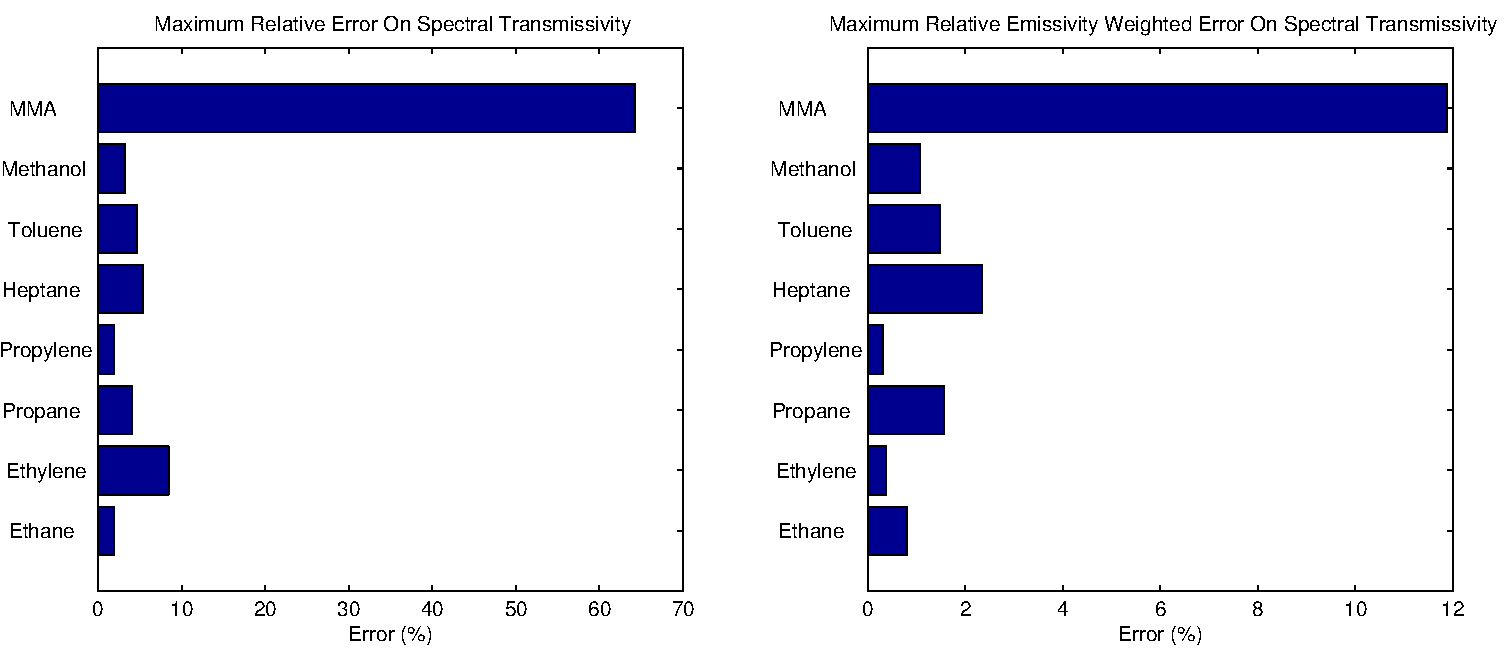
\includegraphics[width=\textwidth]{../Verification/Results_Test2/Test2_Results.pdf}
\end{center}
 \caption{Left: Maximum relative error, in percent, across the whole spectrum and temperature for the new molecules implemented in RadCal. Right: Maximum integrated weighted error (across tested temperatures) calculated using Eq.~\ref{eq:WeightedError}. \label{fig:Verify_All}}
\end{figure}

In the following sections below, for each species, detailed plots comparing the spectral experimental transmissivities with the synthetic ones calculated with RadCal are presented along with plots of the spectral relative error in transmissivity for each pressure-path and temperature tested. Very good agreement is overall found except in some well localized parts of the spectrum for the heaviest molecules and usually at elevated temperature. The reason behind it is that at elevated temperature, the experimental measurements were very close to the optically thin limit, \textit{i.e.} $\tau \rightarrow 1$, and thus some of the measurements were affected by the FTIR sensitivity. Nevertheless, when comparing integrated quantities, \textit{e.g.} the integrated weighted error, the match between experimental and predicted results is very good.


\clearpage

\section{Ethylene: $\rm C_2H_4$}

\begin{figure}[h]
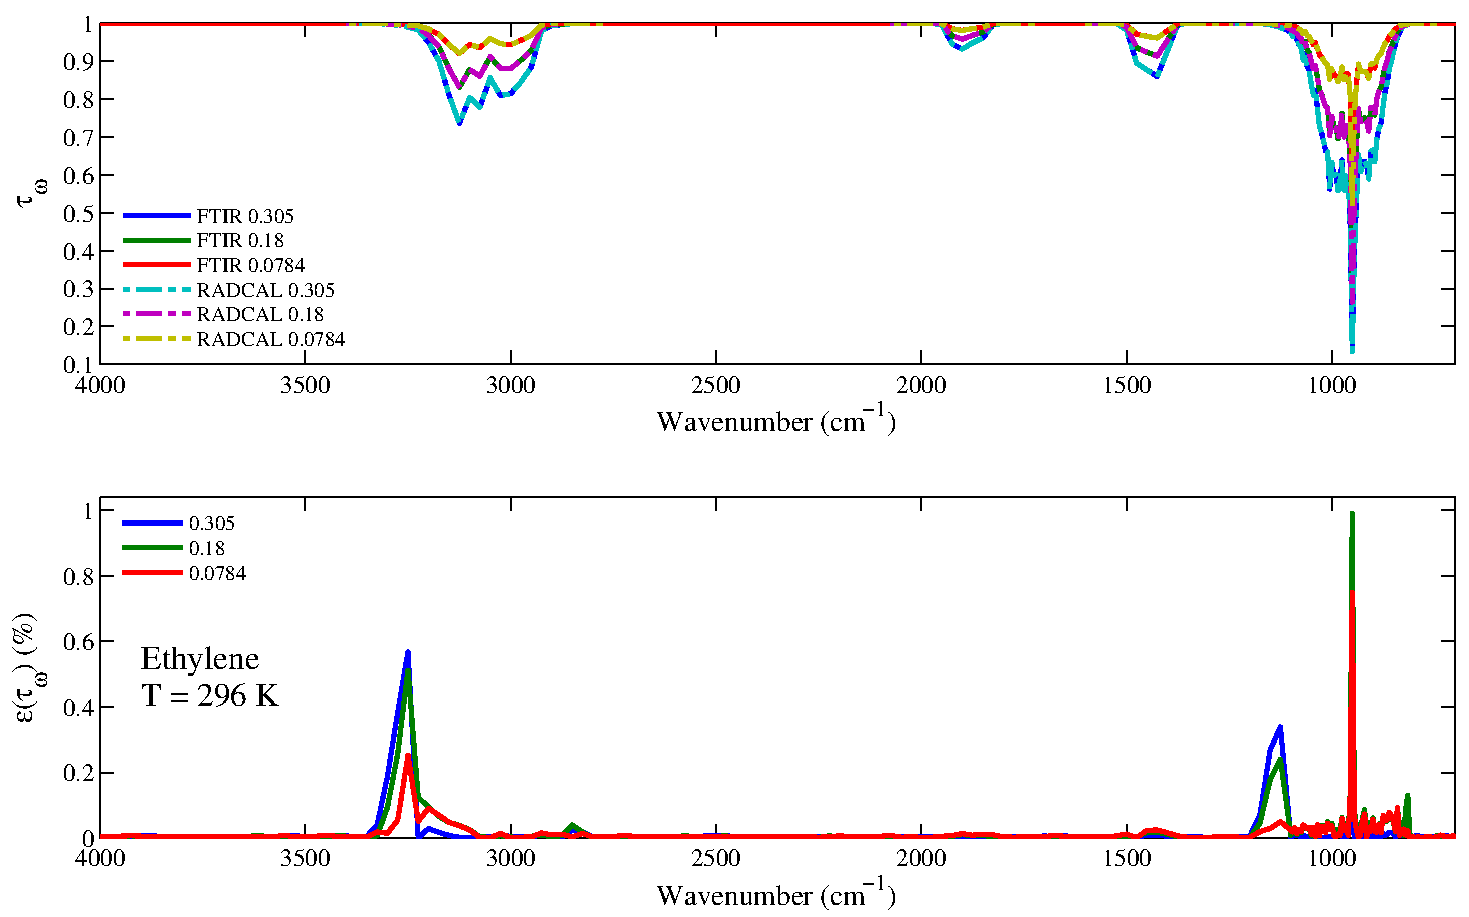
\includegraphics[width=\textwidth]{../Verification/Results_Test2/Ethylene_296.pdf}
\caption{Top: comparison between the experimental (solid lines) and RadCal-generated synthetic (dashed lines) spectral transmissivity profiles, denoted $\tau_{\omega}$, of ethylene of an isothermal homogeneous column of ethylene. Bottom: relative transmissivity error, denoted $\epsilon{(\tau_{\omega})}$, between the experiment and the synthetic profiles presented on the top figure. Three different pressure path lengths are considered: 0.305, 0.18, and 0.0784 atm.cm. The gas temperature is set at 296~K and the total pressure is 101 kPa. Note: the experimental data resolution has been changed to match that of the narrow band model. \label{fig:ethylene_Verify_296K}}
\end{figure}

\newpage

\begin{figure}[p]
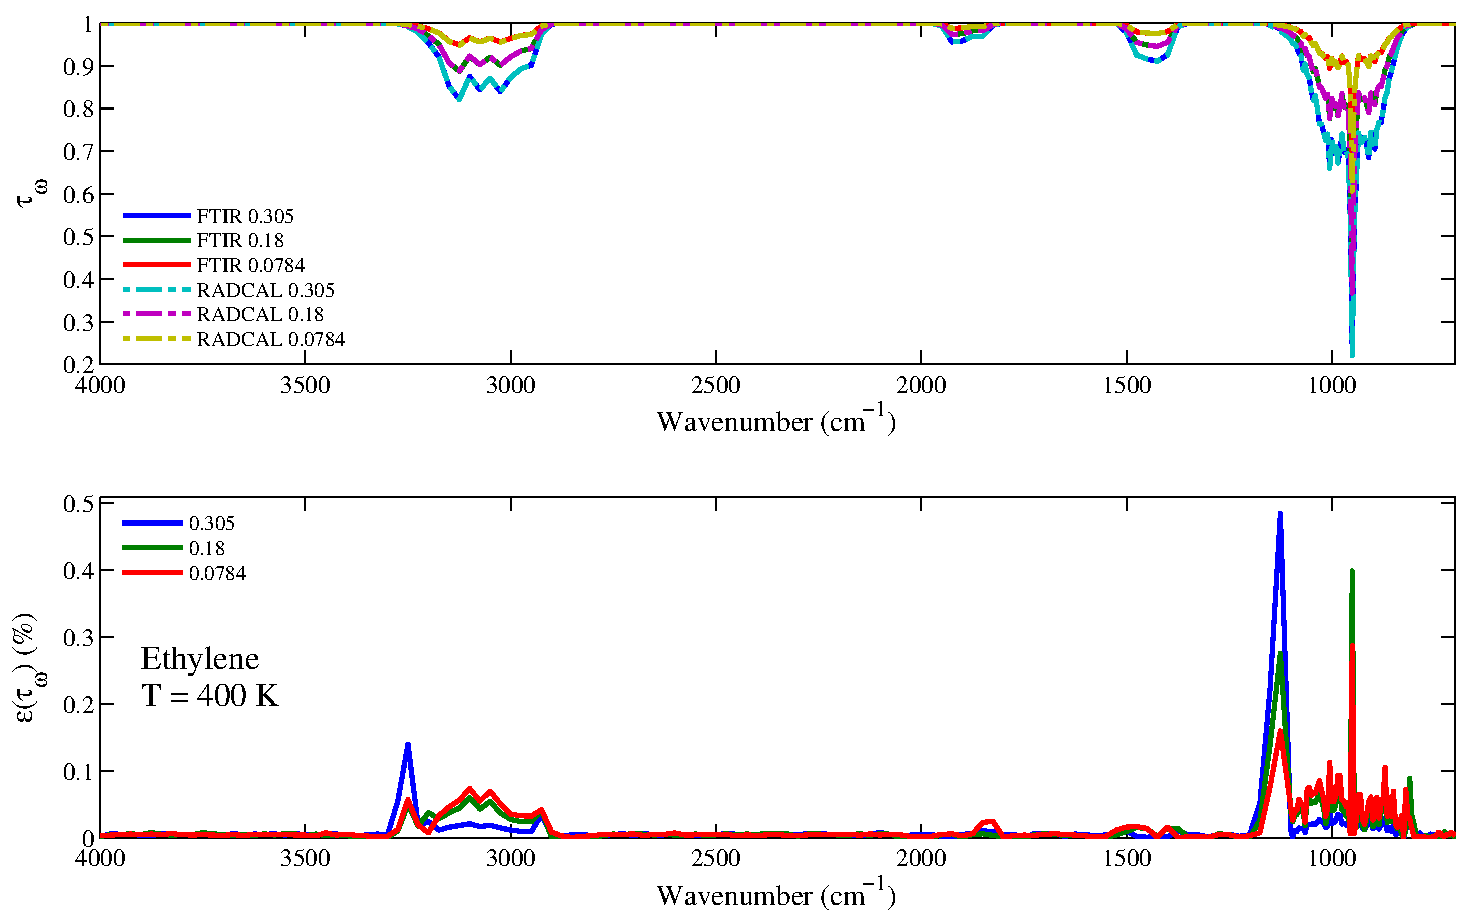
\includegraphics[width=\textwidth]{../Verification/Results_Test2/Ethylene_400.pdf}
\caption{Top: comparison between the experimental (solid lines) and RadCal-generated synthetic (dashed lines) spectral transmissivity profiles, denoted $\tau_{\omega}$, of ethylene of an isothermal homogeneous column of ethylene. Bottom: relative transmissivity error, denoted $\epsilon{(\tau_{\omega})}$, between the experiment and the synthetic profiles presented on the top figure. Three different pressure path lengths are considered: 0.305, 0.18, and 0.0784 atm.cm. The gas temperature is set at 400~K and the total pressure is 101 kPa. Note: the experimental data resolution has been changed to match that of the narrow band model. \label{fig:ethylene_Verify_400K}}
\end{figure}

\begin{figure}[p]
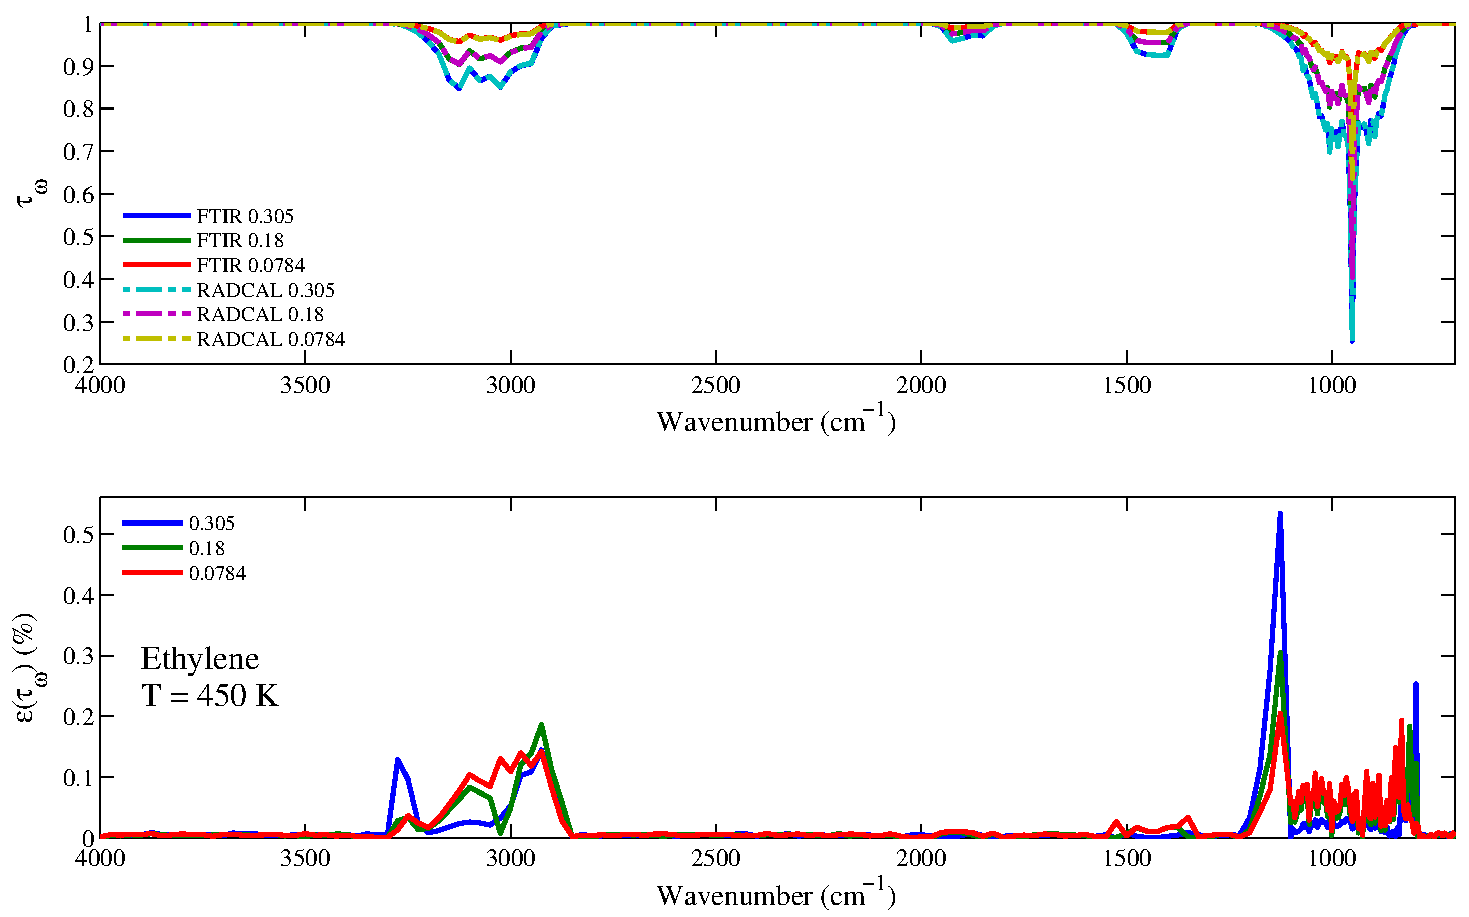
\includegraphics[width=\textwidth]{../Verification/Results_Test2/Ethylene_450.pdf}
\caption{Top: comparison between the experimental (solid lines) and RadCal-generated synthetic (dashed lines) spectral transmissivity profiles, denoted $\tau_{\omega}$, of ethylene of an isothermal homogeneous column of ethylene. Bottom: relative transmissivity error, denoted $\epsilon{(\tau_{\omega})}$, between the experiment and the synthetic profiles presented on the top figure. Three different pressure path lengths are considered: 0.305, 0.18, and 0.0784 atm.cm. The gas temperature is set at 450~K and the total pressure is 101 kPa. Note: the experimental data resolution has been changed to match that of the narrow band model. \label{fig:ethylene_Verify_450K}}
\end{figure}

\begin{figure}[p]
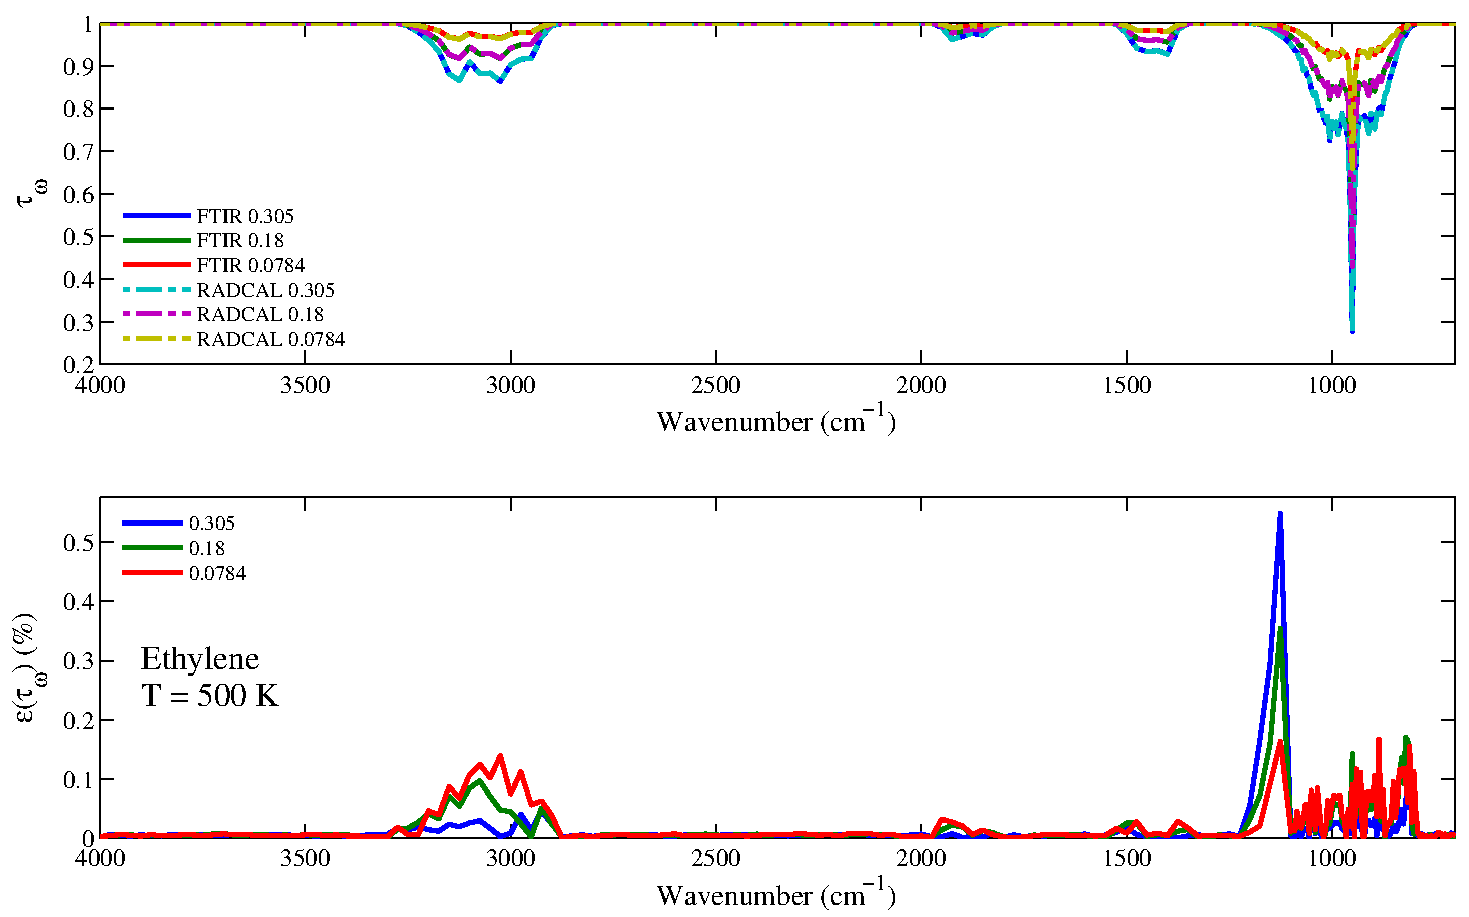
\includegraphics[width=\textwidth]{../Verification/Results_Test2/Ethylene_500.pdf}
\caption{Top: comparison between the experimental (solid lines) and RadCal-generated synthetic (dashed lines) spectral transmissivity profiles, denoted $\tau_{\omega}$, of ethylene of an isothermal homogeneous column of ethylene. Bottom: relative transmissivity error, denoted $\epsilon{(\tau_{\omega})}$, between the experiment and the synthetic profiles presented on the top figure. Three different pressure path lengths are considered: 0.305, 0.18, and 0.0784 atm.cm. The gas temperature is set at 500~K and the total pressure is 101 kPa. Note: the experimental data resolution has been changed to match that of the narrow band model. \label{fig:ethylene_Verify_500K}}
\end{figure}

\begin{figure}[p]
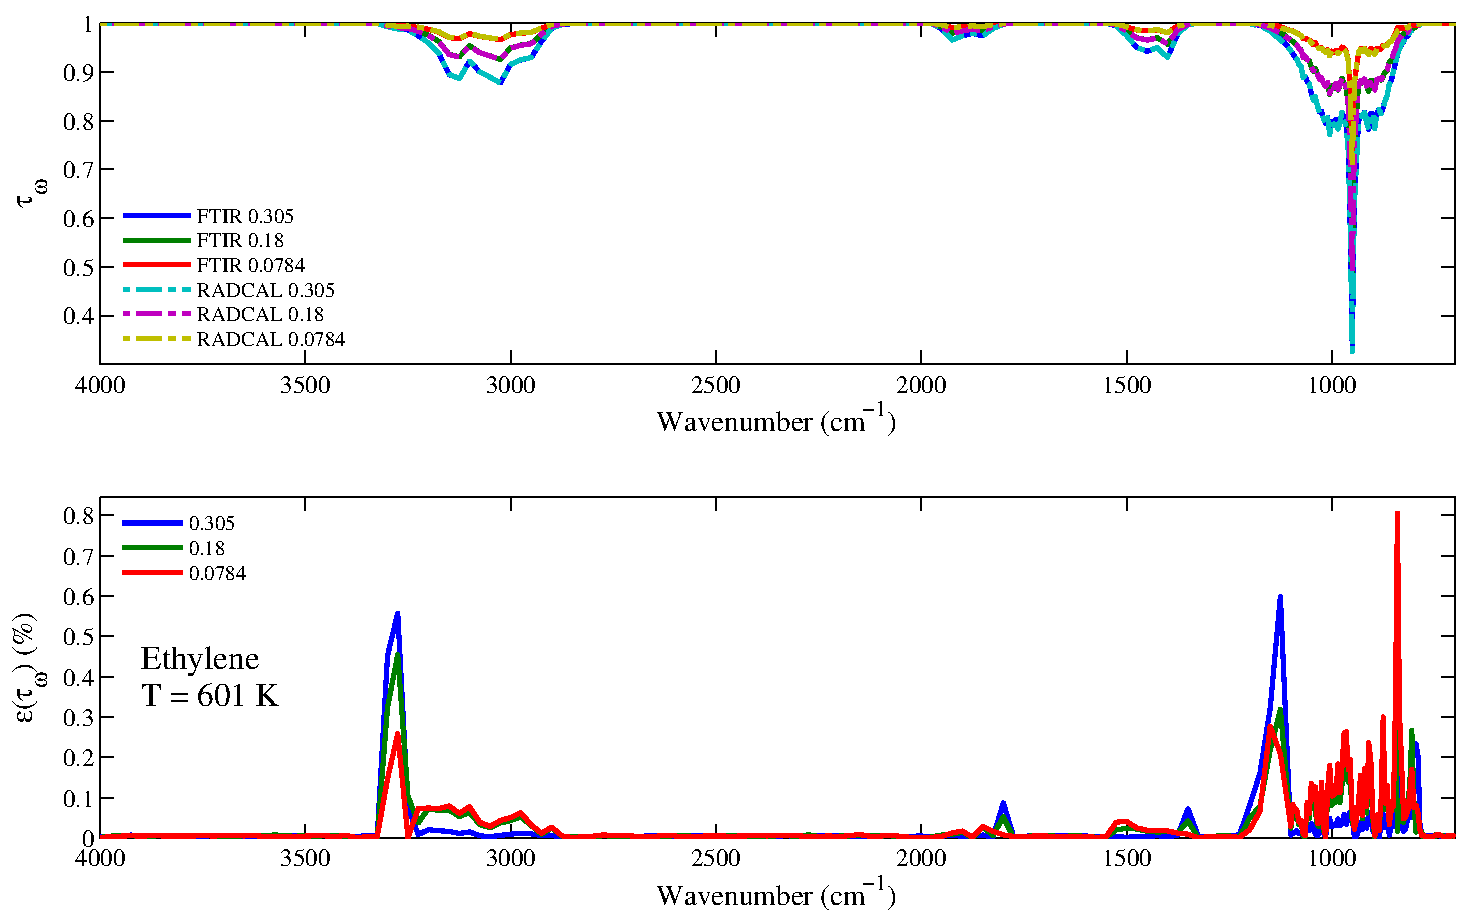
\includegraphics[width=\textwidth]{../Verification/Results_Test2/Ethylene_601.pdf}
\caption{Top: comparison between the experimental (solid lines) and RadCal-generated synthetic (dashed lines) spectral transmissivity profiles, denoted $\tau_{\omega}$, of ethylene of an isothermal homogeneous column of ethylene. Bottom: relative transmissivity error, denoted $\epsilon{(\tau_{\omega})}$, between the experiment and the synthetic profiles presented on the top figure. Three different pressure path lengths are considered: 0.305, 0.18, and 0.0784 atm.cm. The gas temperature is set at 601~K and the total pressure is 101 kPa. Note: the experimental data resolution has been changed to match that of the narrow band model. \label{fig:ethylene_Verify_600K}}
\end{figure}

\begin{figure}[p]
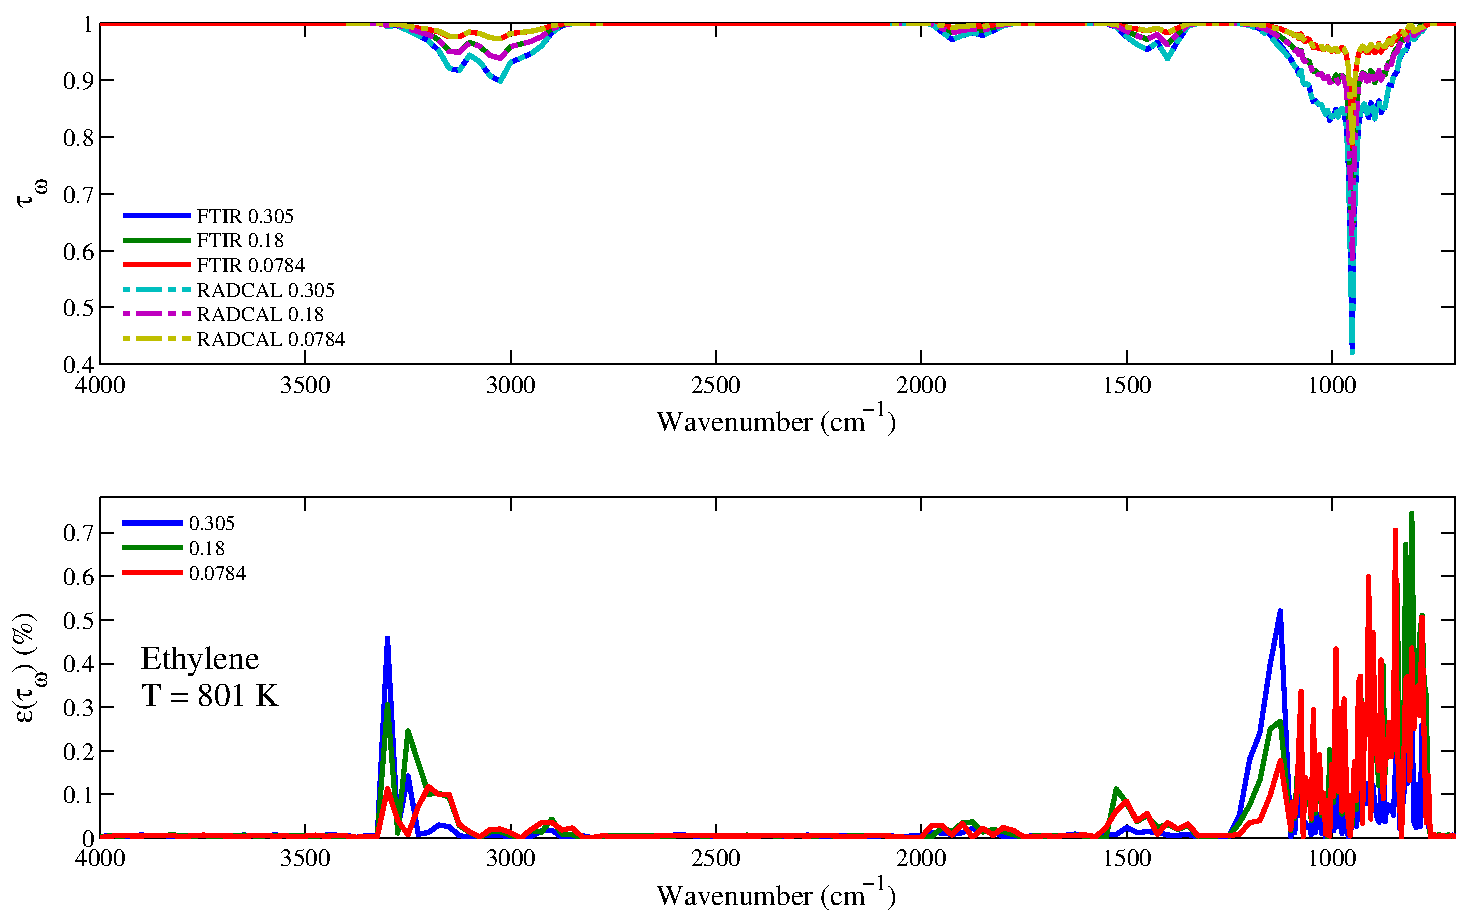
\includegraphics[width=\textwidth]{../Verification/Results_Test2/Ethylene_801.pdf}
\caption{Top: comparison between the experimental (solid lines) and RadCal-generated synthetic (dashed lines) spectral transmissivity profiles, denoted $\tau_{\omega}$, of ethylene of an isothermal homogeneous column of ethylene. Bottom: relative transmissivity error, denoted $\epsilon{(\tau_{\omega})}$, between the experiment and the synthetic profiles presented on the top figure. Three different pressure path lengths are considered: 0.305, 0.18, and 0.0784 atm.cm. The gas temperature is set at 801~K and the total pressure is 101 kPa. Note: the experimental data resolution has been changed to match that of the narrow band model. \label{fig:ethylene_Verify_801K}}
\end{figure}

\begin{figure}[p]
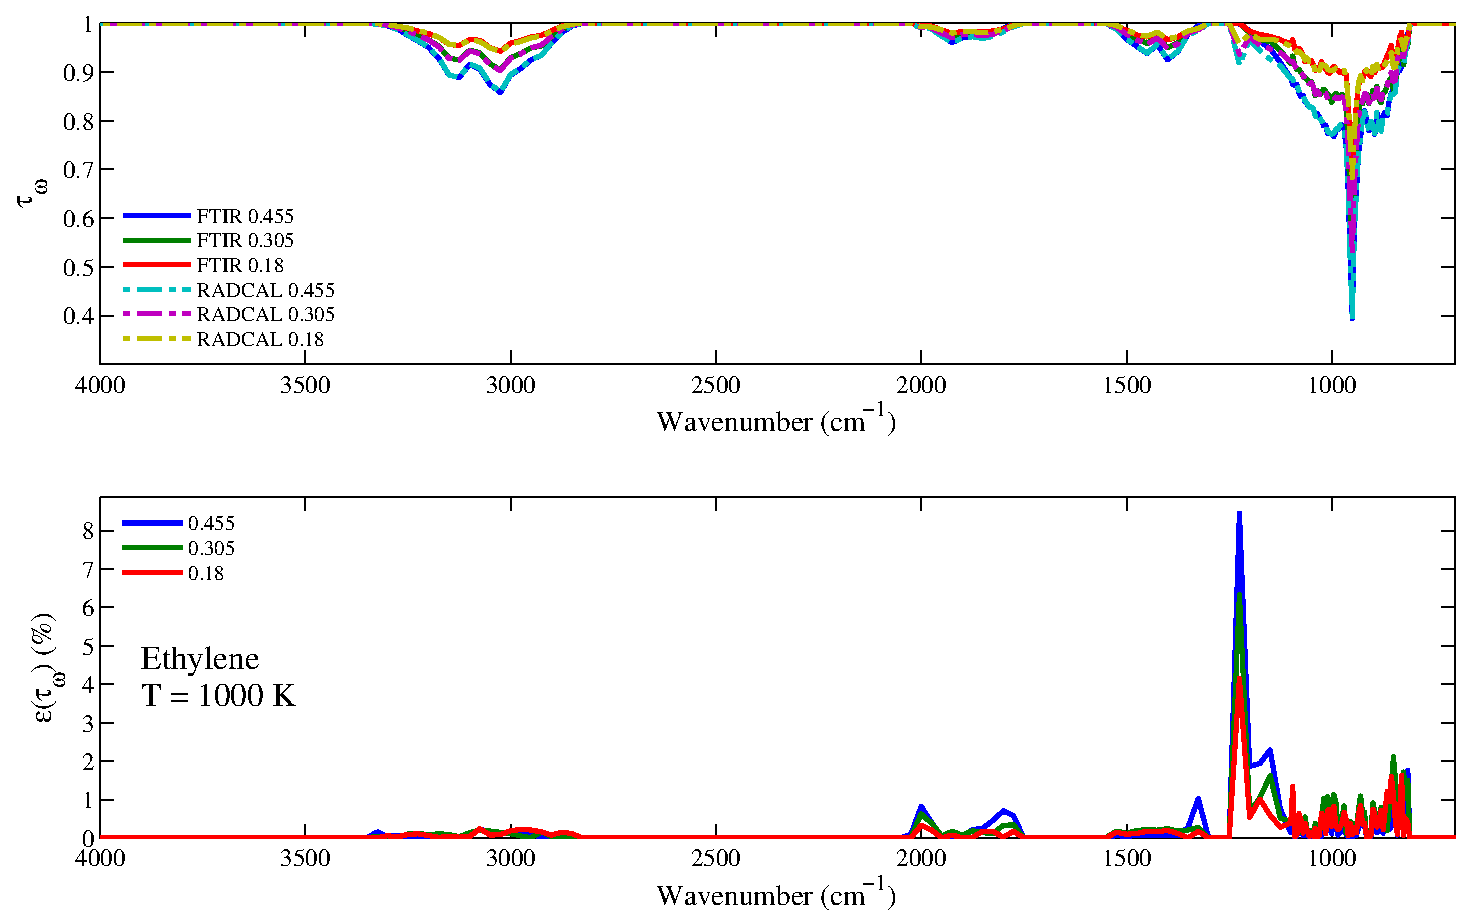
\includegraphics[width=\textwidth]{../Verification/Results_Test2/Ethylene_1000.pdf}
\caption{Top: comparison between the experimental (solid lines) and RadCal-generated synthetic (dashed lines) spectral transmissivity profiles, denoted $\tau_{\omega}$, of ethylene of an isothermal homogeneous column of ethylene. Bottom: relative transmissivity error, denoted $\epsilon{(\tau_{\omega})}$, between the experiment and the synthetic profiles presented on the top figure. Three different pressure path lengths are considered: 0.305, 0.18, and 0.0784 atm.cm. The gas temperature is set at 1000~K and the total pressure is 101 kPa. Note: the experimental data resolution has been changed to match that of the narrow band model. \label{fig:ethylene_Verify_1000K}}
\end{figure}


\clearpage

\section{Ethane: $\rm C_2H_6$}

\begin{figure}[h]
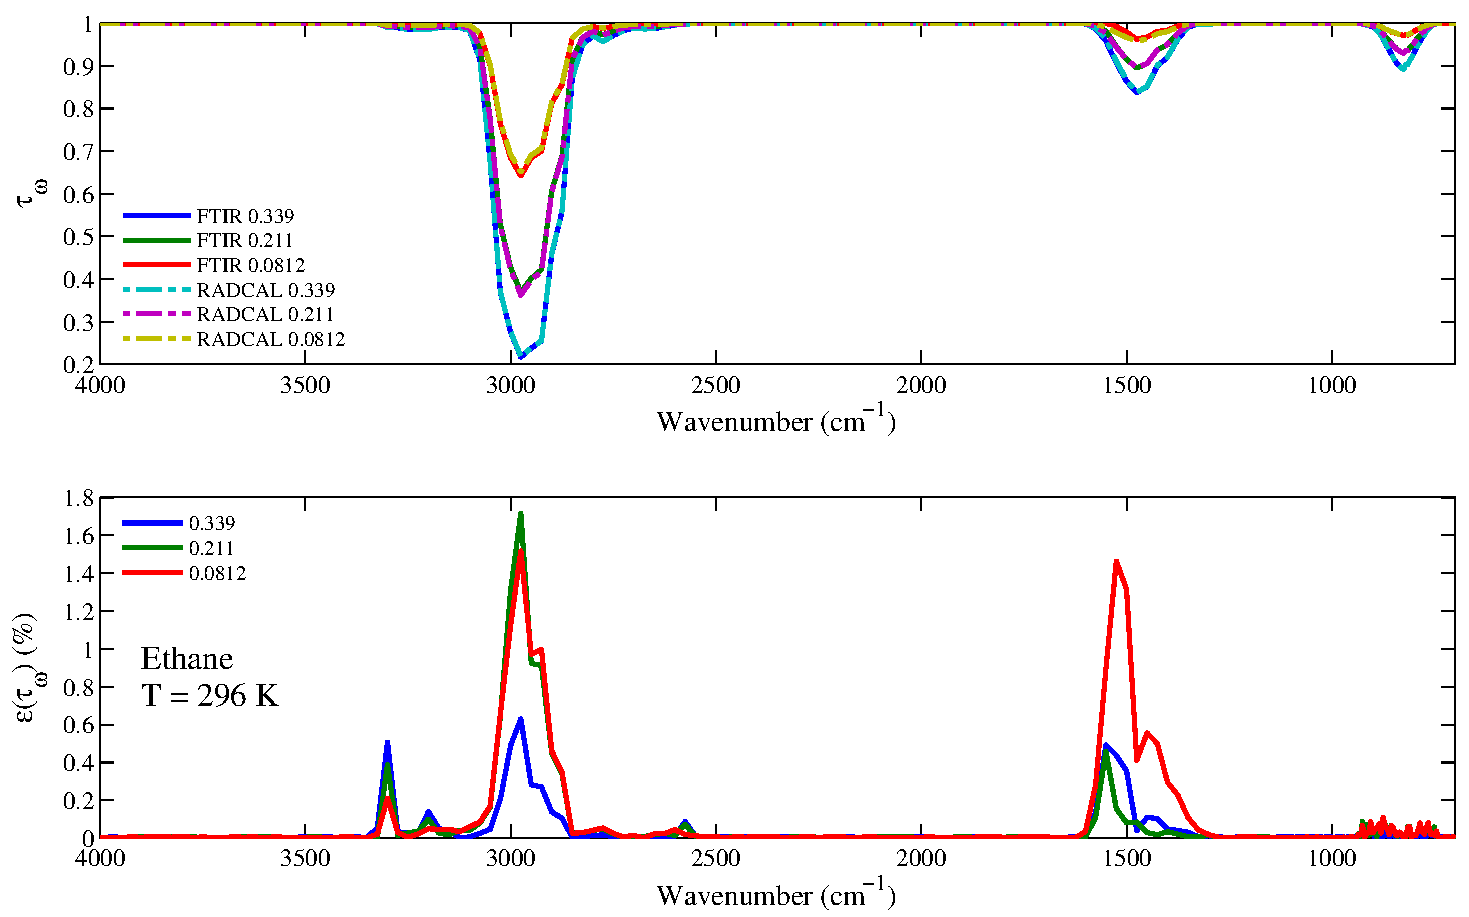
\includegraphics[width=\textwidth]{../Verification/Results_Test2/Ethane_296.pdf}
\caption{Top: comparison between the experimental (solid lines) and RadCal-generated synthetic (dashed lines) spectral transmissivity profiles, denoted $\tau_{\omega}$, of ethane of an isothermal homogeneous column of ethane. Bottom: relative transmissivity error, denoted $\epsilon{(\tau_{\omega})}$, between the experiment and the synthetic profiles presented on the top figure. Three different pressure path lengths are considered: 0.339, 0.211, and 0.0812 atm.cm. The gas temperature is set at 296~K and the total pressure is 101 kPa. Note: the experimental data resolution has been changed to match that of the narrow band model. \label{fig:ethane_Verify_296K}}
\end{figure}

\newpage

\begin{figure}[p]
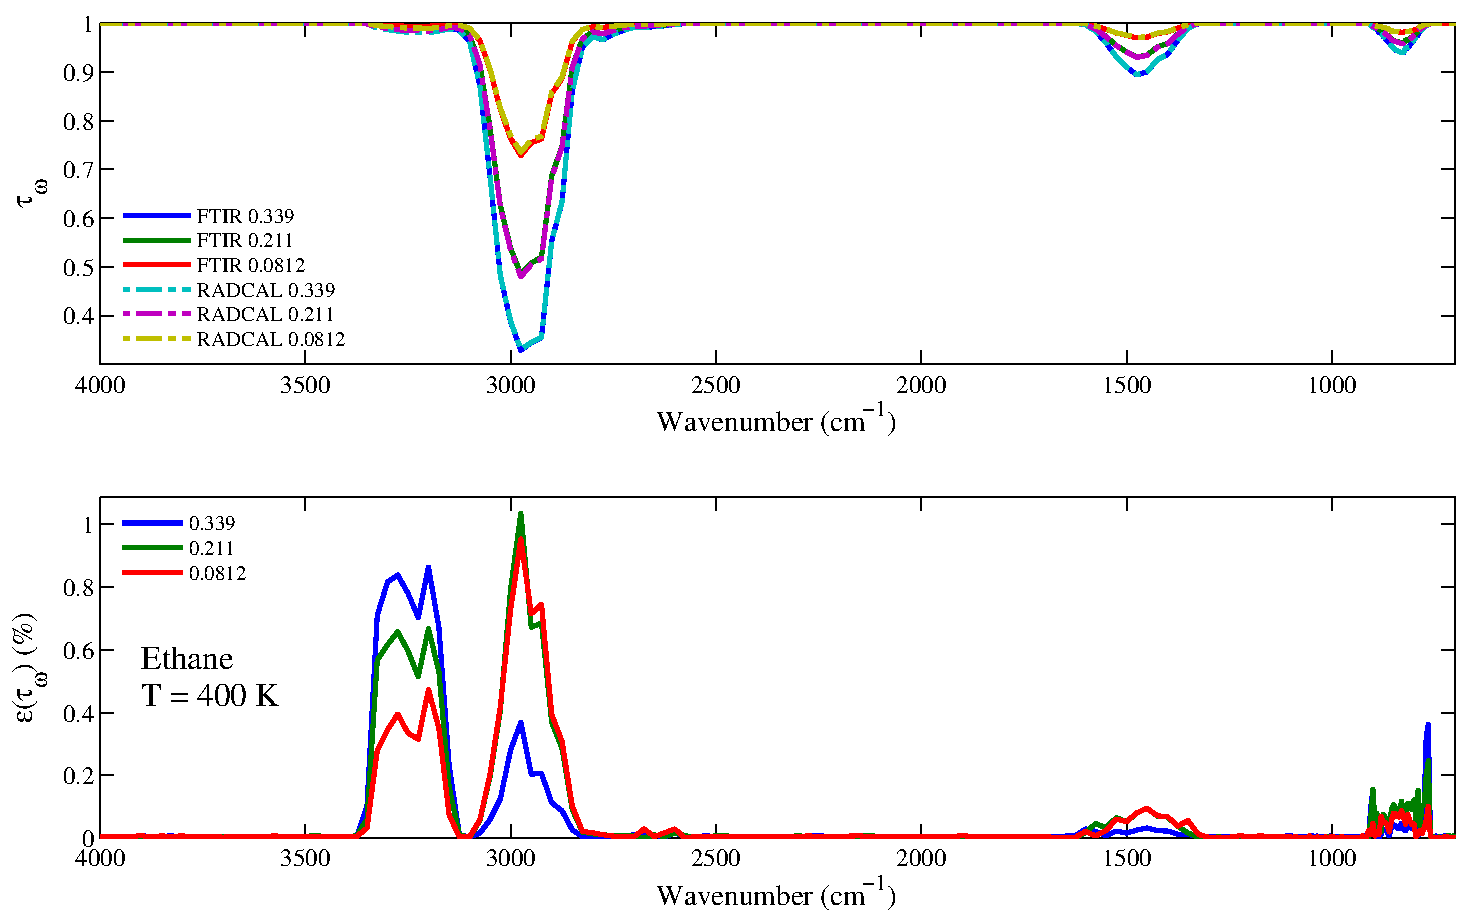
\includegraphics[width=\textwidth]{../Verification/Results_Test2/Ethane_400.pdf}
\caption{Top: comparison between the experimental (solid lines) and RadCal-generated synthetic (dashed lines) spectral transmissivity profiles, denoted $\tau_{\omega}$, of ethane of an isothermal homogeneous column of ethane. Bottom: relative transmissivity error, denoted $\epsilon{(\tau_{\omega})}$, between the experiment and the synthetic profiles presented on the top figure. Three different pressure path lengths are considered: 0.339, 0.211, and 0.0812 atm.cm. The gas temperature is set at 400~K and the total pressure is 101 kPa. Note: the experimental data resolution has been changed to match that of the narrow band model. \label{fig:ethane_Verify_400K}}
\end{figure}

\begin{figure}[p]
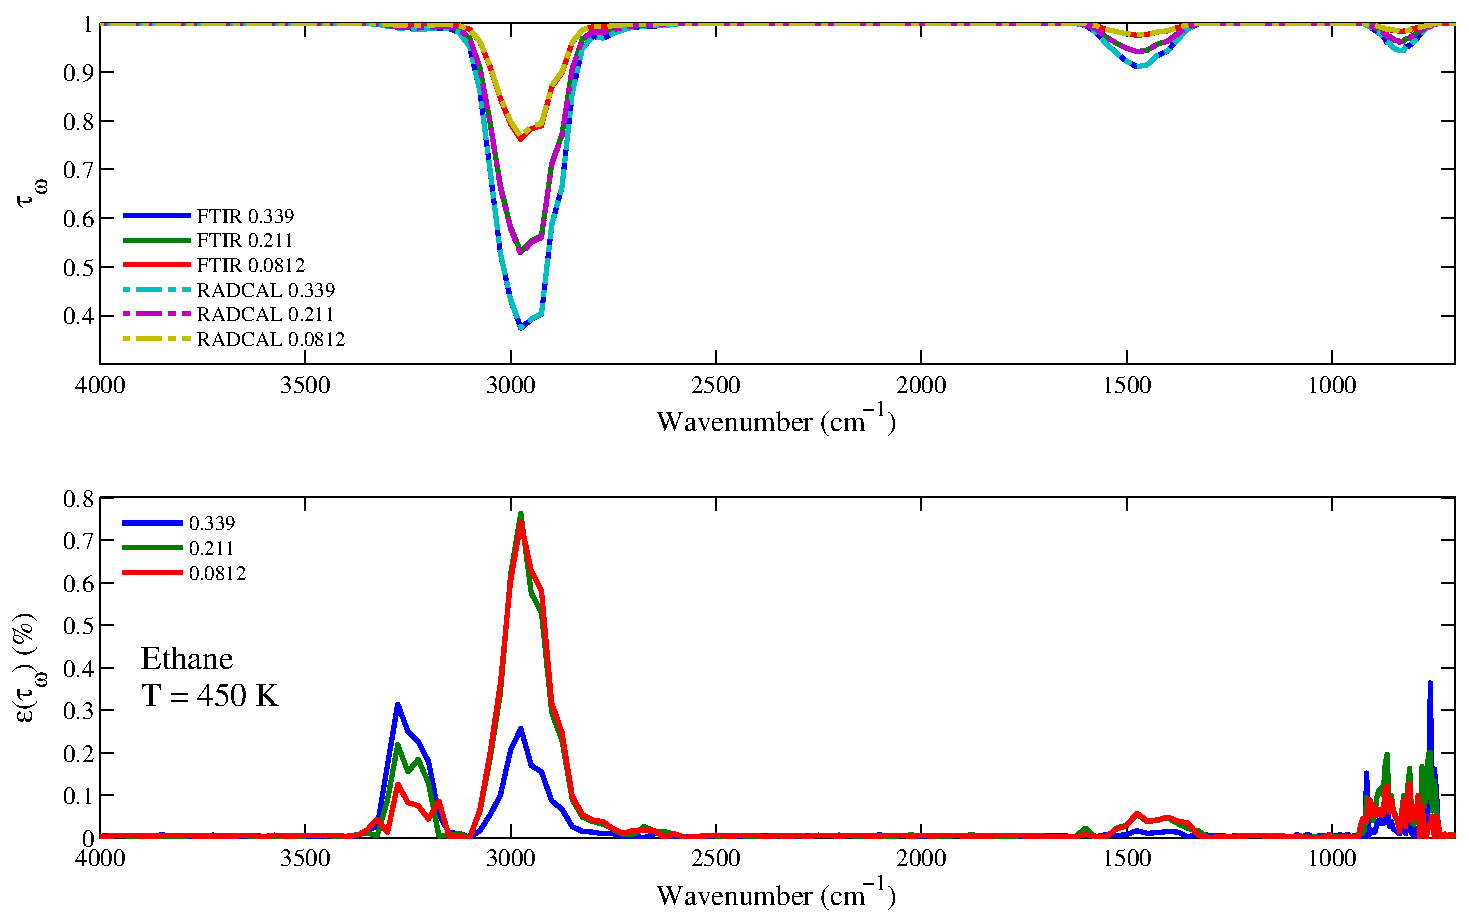
\includegraphics[width=\textwidth]{../Verification/Results_Test2/Ethane_450.pdf}
\caption{Top: comparison between the experimental (solid lines) and RadCal-generated synthetic (dashed lines) spectral transmissivity profiles, denoted $\tau_{\omega}$, of ethane of an isothermal homogeneous column of ethane. Bottom: relative transmissivity error, denoted $\epsilon{(\tau_{\omega})}$, between the experiment and the synthetic profiles presented on the top figure. Three different pressure path lengths are considered: 0.339, 0.211, and 0.0812 atm.cm. The gas temperature is set at 450~K and the total pressure is 101 kPa. Note: the experimental data resolution has been changed to match that of the narrow band model. \label{fig:ethane_Verify_450K}}
\end{figure}

\begin{figure}[p]
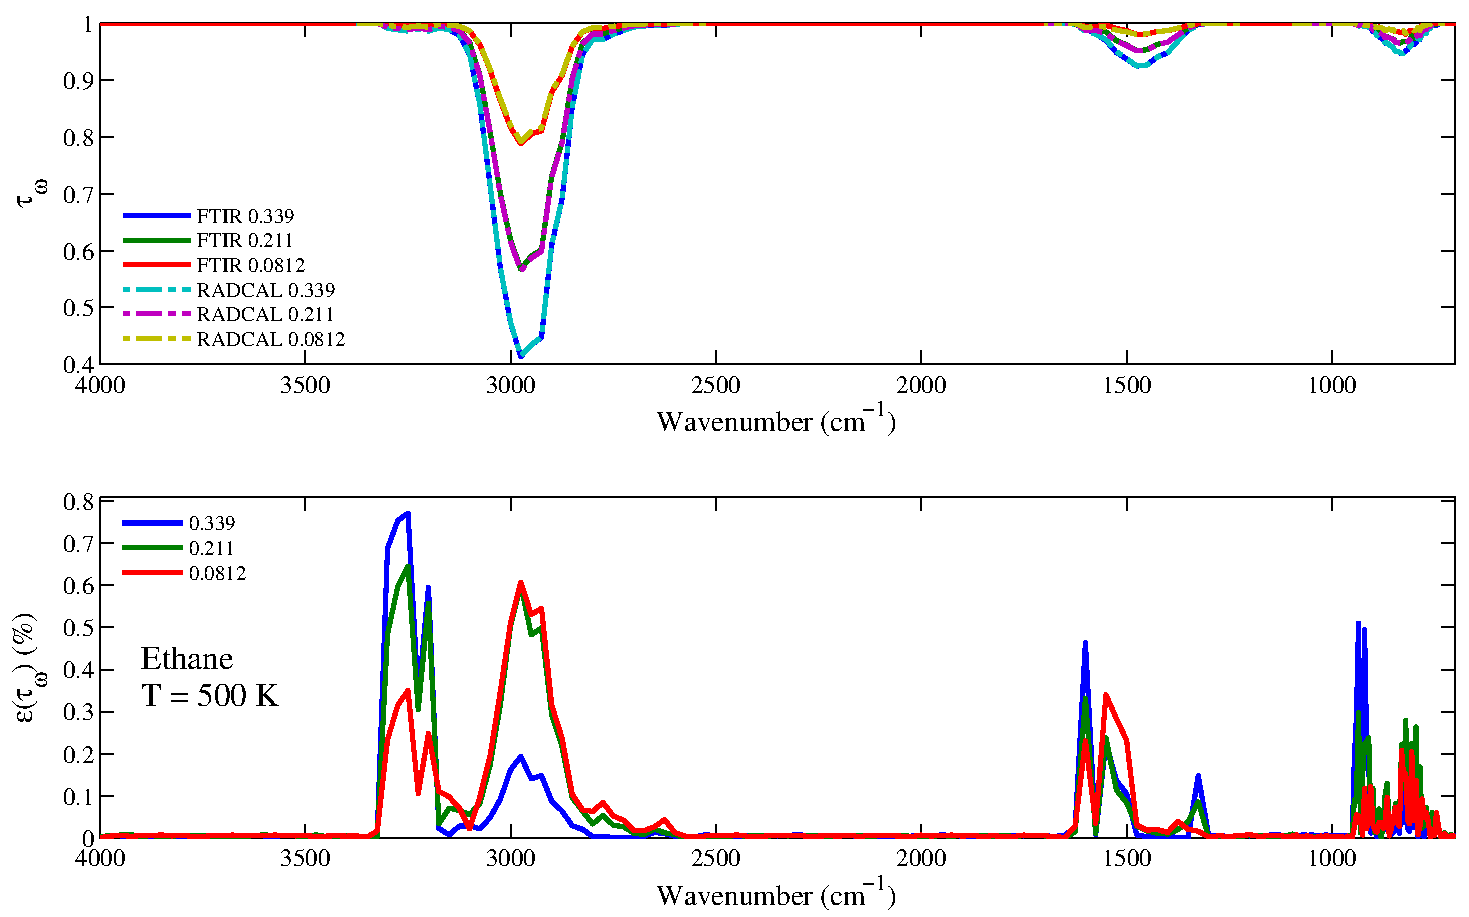
\includegraphics[width=\textwidth]{../Verification/Results_Test2/Ethane_500.pdf}
\caption{Top: comparison between the experimental (solid lines) and RadCal-generated synthetic (dashed lines) spectral transmissivity profiles, denoted $\tau_{\omega}$, of ethane of an isothermal homogeneous column of ethane. Bottom: relative transmissivity error, denoted $\epsilon{(\tau_{\omega})}$, between the experiment and the synthetic profiles presented on the top figure. Three different pressure path lengths are considered: 0.339, 0.211, and 0.0812 atm.cm. The gas temperature is set at 500~K and the total pressure is 101 kPa. Note: the experimental data resolution has been changed to match that of the narrow band model. \label{fig:ethane_Verify_500K}}
\end{figure}

\begin{figure}[p]
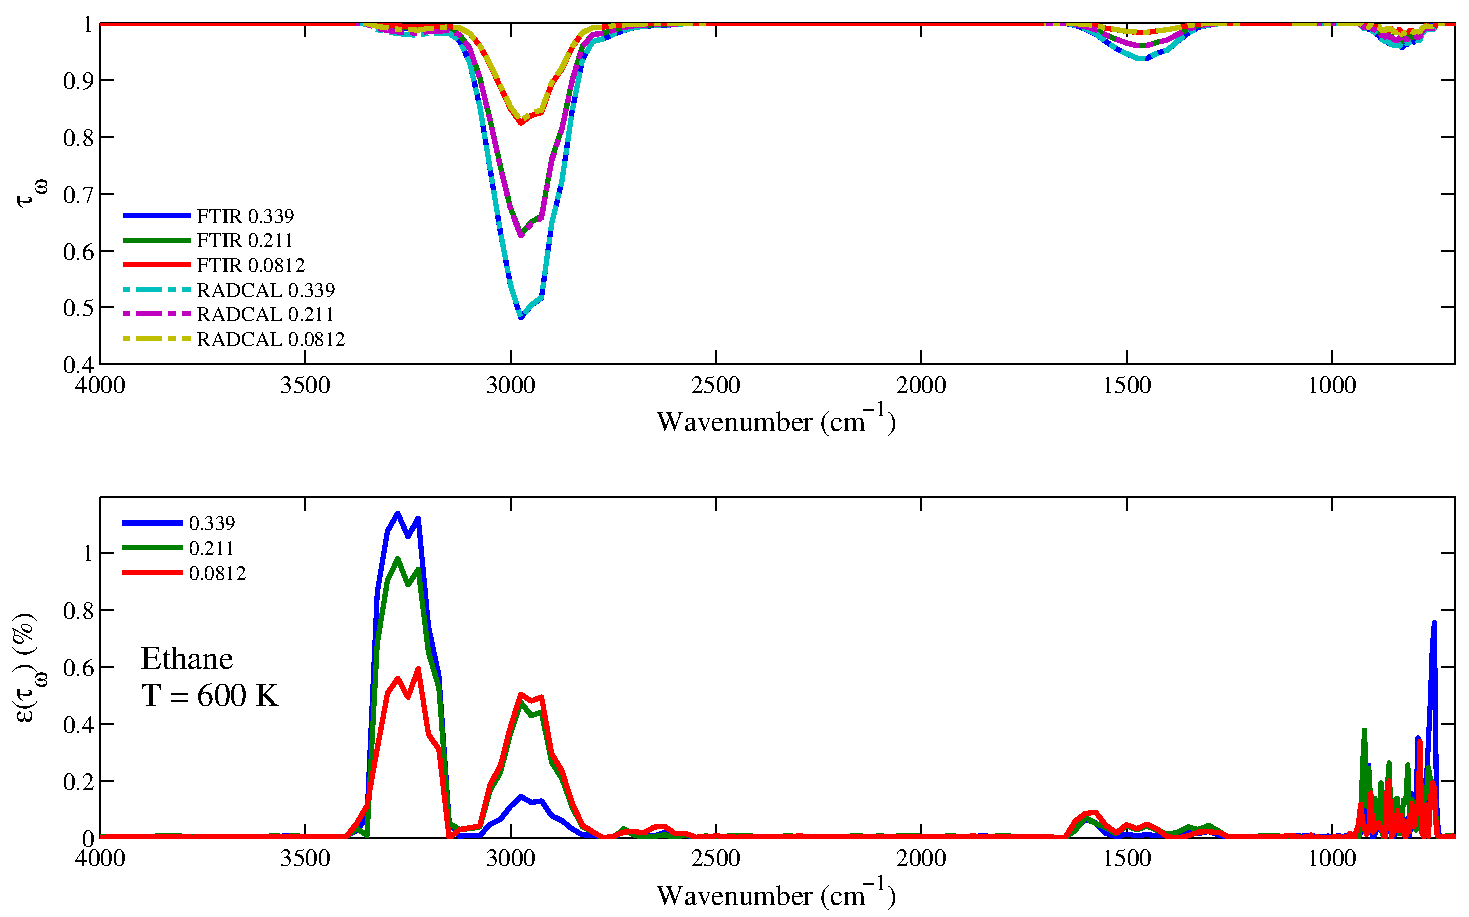
\includegraphics[width=\textwidth]{../Verification/Results_Test2/Ethane_600.pdf}
\caption{Top: comparison between the experimental (solid lines) and RadCal-generated synthetic (dashed lines) spectral transmissivity profiles, denoted $\tau_{\omega}$, of ethane of an isothermal homogeneous column of ethane. Bottom: relative transmissivity error, denoted $\epsilon{(\tau_{\omega})}$, between the experiment and the synthetic profiles presented on the top figure. Three different pressure path lengths are considered: 0.339, 0.211, and 0.0812 atm.cm. The gas temperature is set at 600~K and the total pressure is 101 kPa. Note: the experimental data resolution has been changed to match that of the narrow band model. \label{fig:ethane_Verify_600K}}
\end{figure}

\begin{figure}[p]
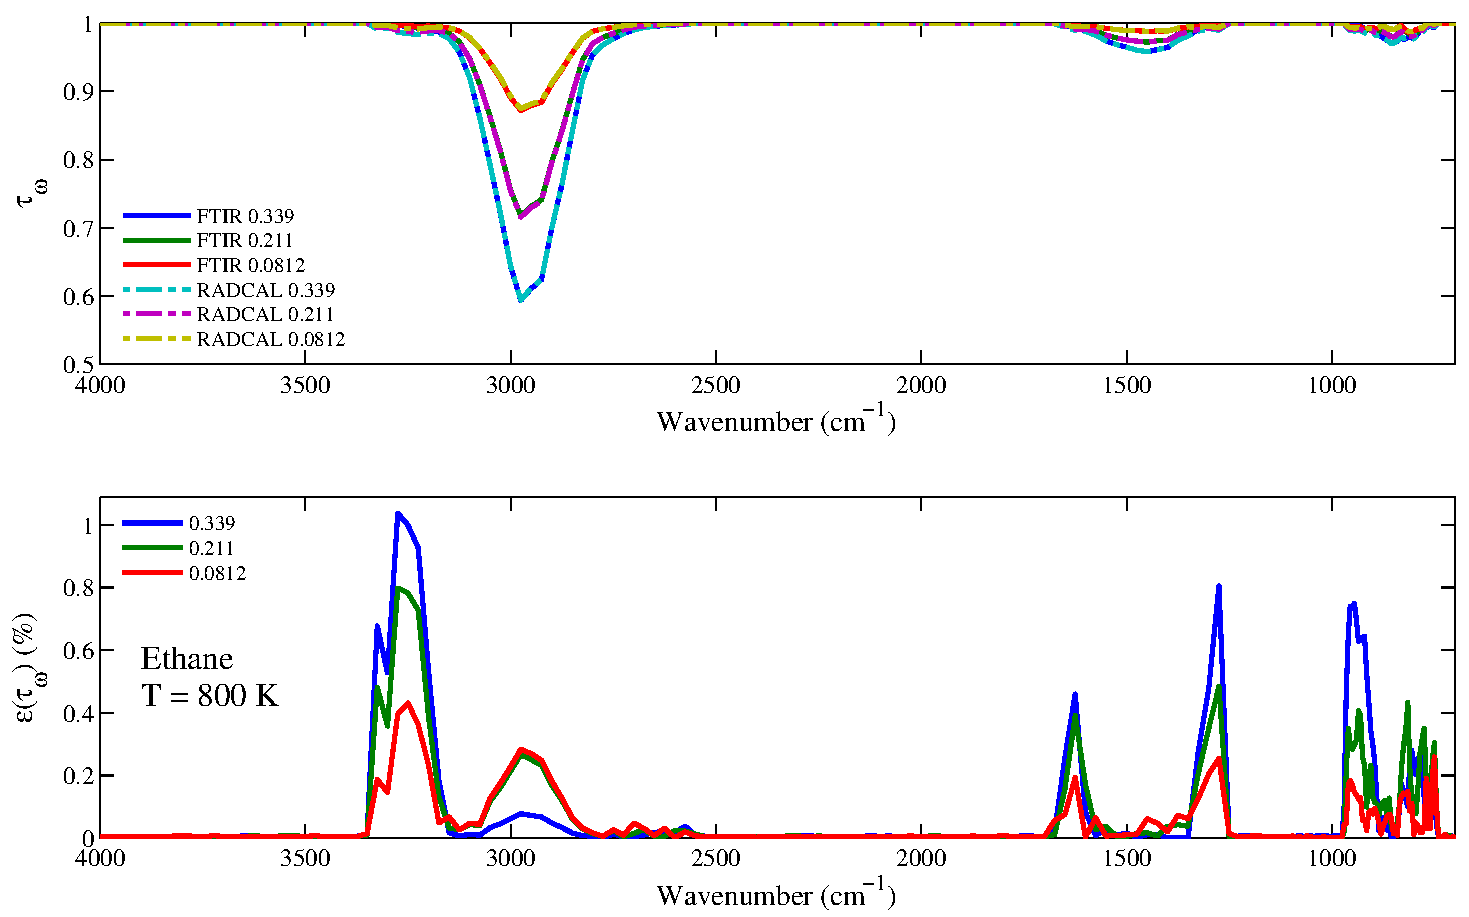
\includegraphics[width=\textwidth]{../Verification/Results_Test2/Ethane_800.pdf}
\caption{Top: comparison between the experimental (solid lines) and RadCal-generated synthetic (dashed lines) spectral transmissivity profiles, denoted $\tau_{\omega}$, of ethane of an isothermal homogeneous column of ethane. Bottom: relative transmissivity error, denoted $\epsilon{(\tau_{\omega})}$, between the experiment and the synthetic profiles presented on the top figure. Three different pressure path lengths are considered: 0.339, 0.211, and 0.0812 atm.cm. The gas temperature is set at 801~K and the total pressure is 101 kPa. Note: the experimental data resolution has been changed to match that of the narrow band model. \label{fig:ethane_Verify_800K}}
\end{figure}

\begin{figure}[p]
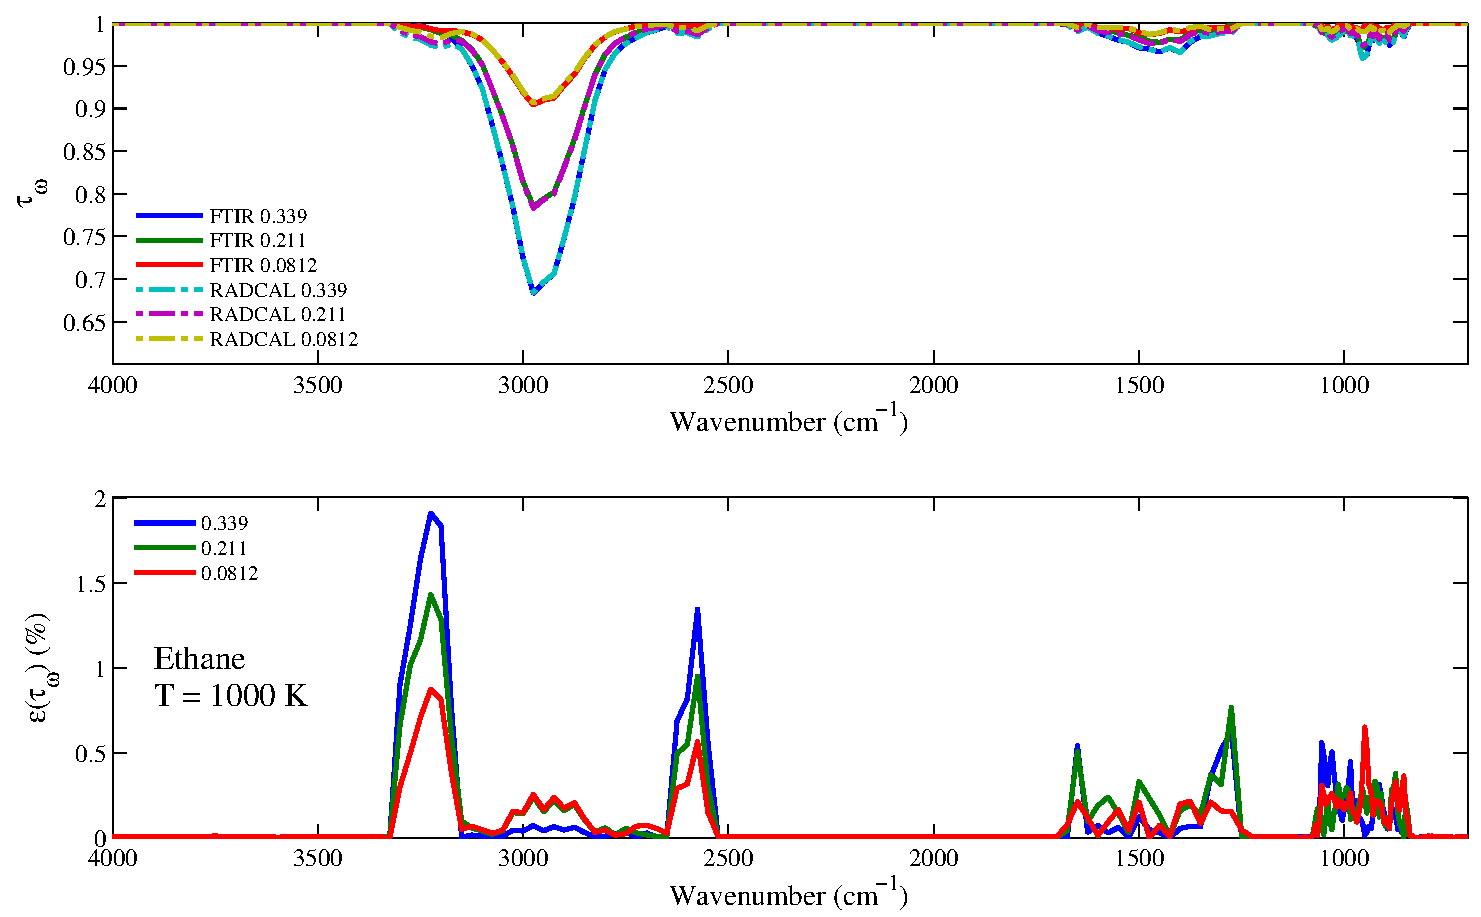
\includegraphics[width=\textwidth]{../Verification/Results_Test2/Ethane_1000.pdf}
\caption{Top: comparison between the experimental (solid lines) and RadCal-generated synthetic (dashed lines) spectral transmissivity profiles, denoted $\tau_{\omega}$, of ethane of an isothermal homogeneous column of ethane. Bottom: relative transmissivity error, denoted $\epsilon{(\tau_{\omega})}$, between the experiment and the synthetic profiles presented on the top figure. Three different pressure path lengths are considered: 0.339, 0.211, and 0.0812 atm.cm. The gas temperature is set at 1000~K and the total pressure is 101 kPa. Note: the experimental data resolution has been changed to match that of the narrow band model. \label{fig:ethane_Verify_1000K}}
\end{figure}


\clearpage

\section{Propylene: $\rm C_3H_6$}

\begin{figure}[h]
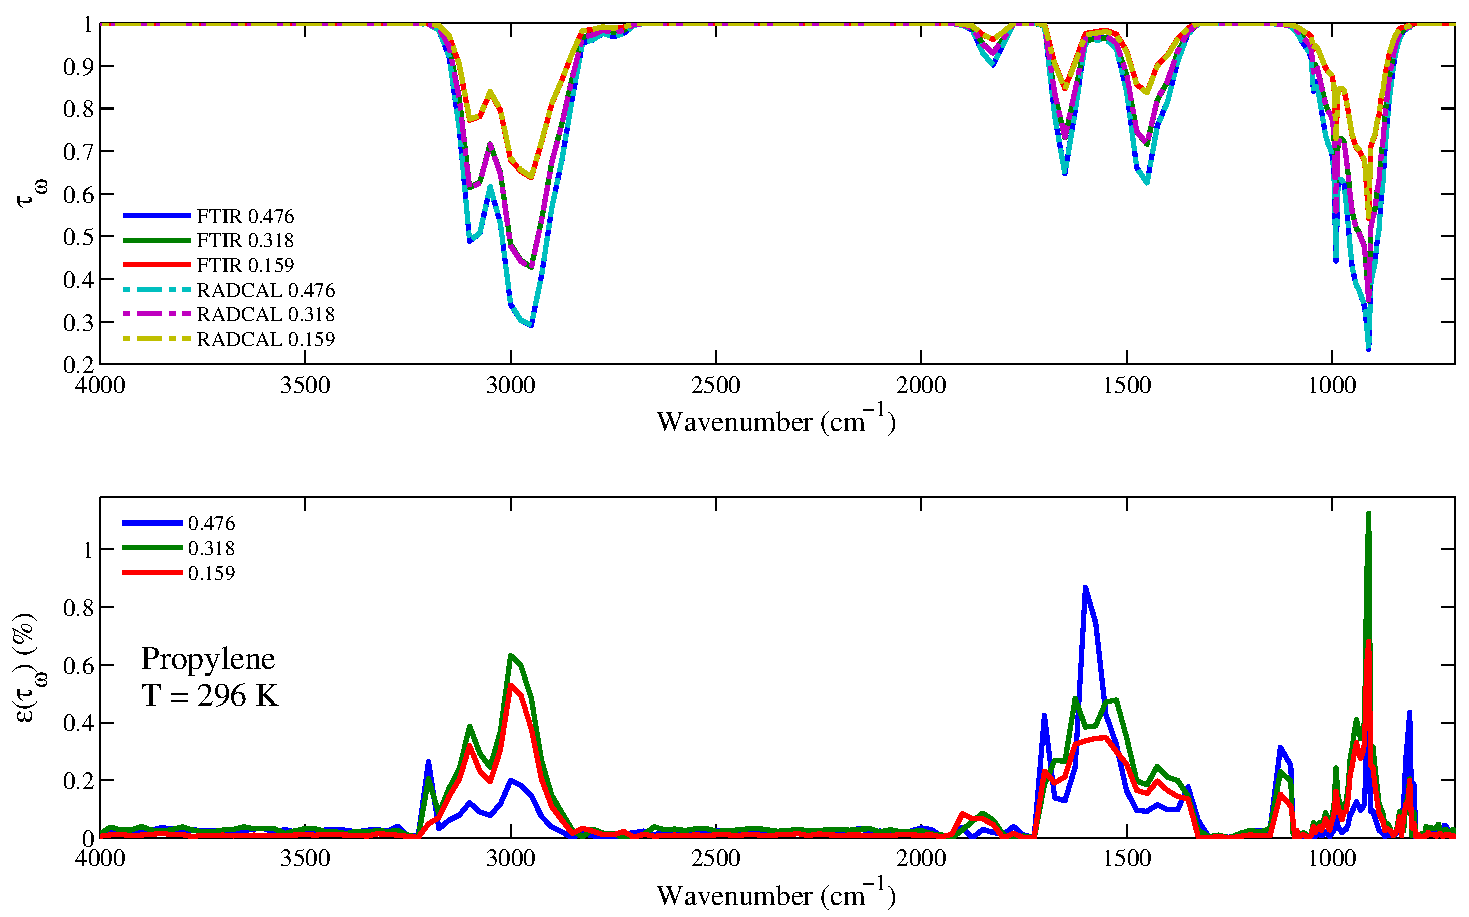
\includegraphics[width=\textwidth]{../Verification/Results_Test2/Propylene_296.pdf}
\caption{Top: comparison between the experimental (solid lines) and RadCal-generated synthetic (dashed lines) spectral transmissivity profiles, denoted $\tau_{\omega}$, of propylene of an isothermal homogeneous column of propylene. Bottom: relative transmissivity error, denoted $\epsilon{(\tau_{\omega})}$, between the experiment and the synthetic profiles presented on the top figure. Three different pressure path lengths are considered: 0.476, 0.318, and 0.159 atm.cm. The gas temperature is set at 296~K and the total pressure is 101 kPa. Note: the experimental data resolution has been changed to match that of the narrow band model. \label{fig:propylene_Verify_296K}}
\end{figure}

\newpage

\begin{figure}[p]
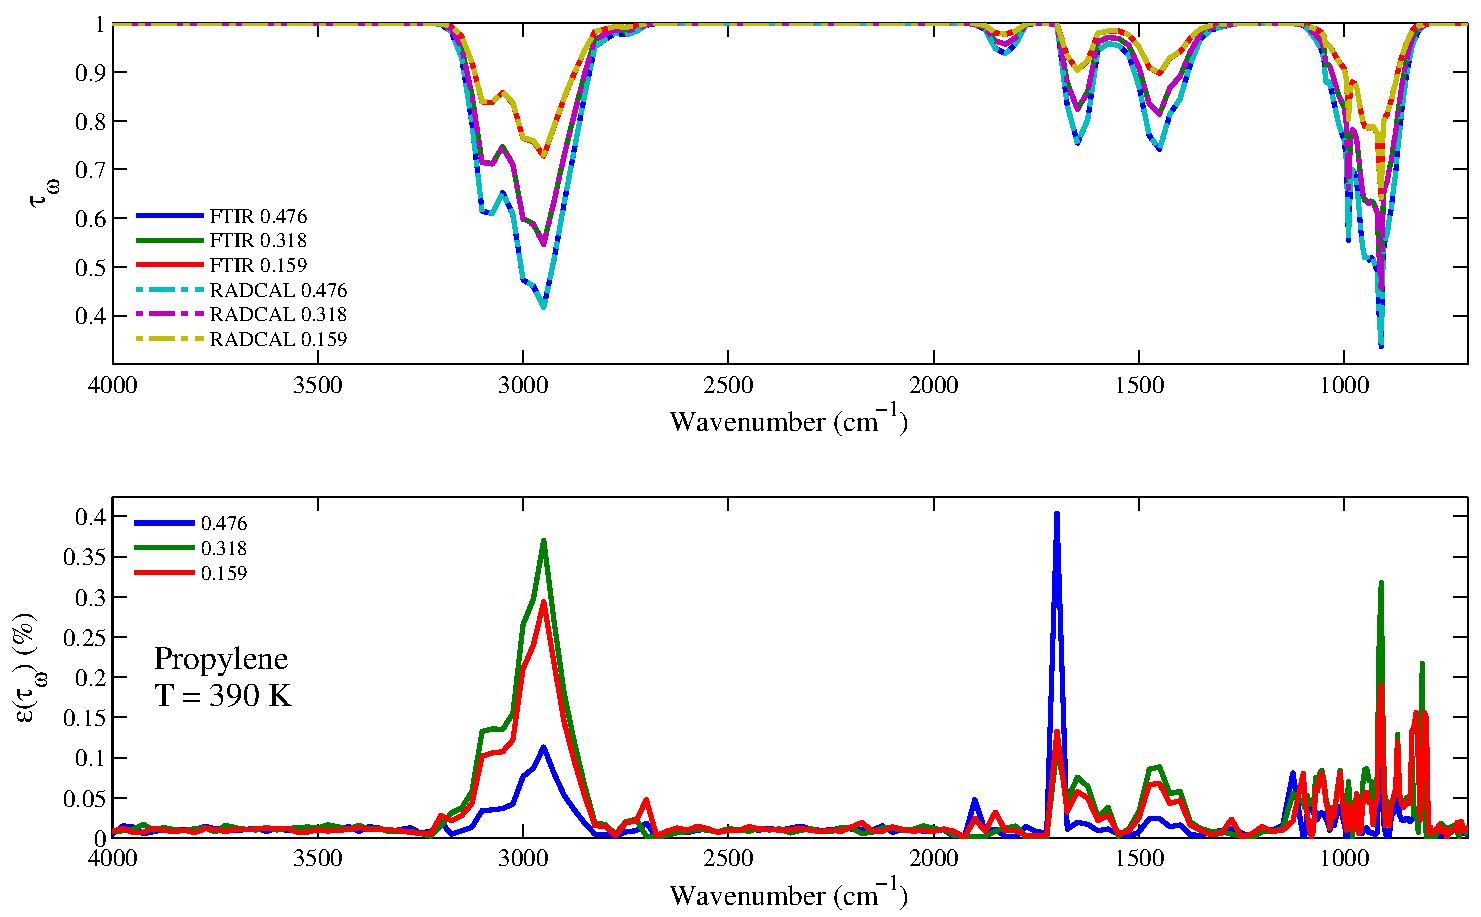
\includegraphics[width=\textwidth]{../Verification/Results_Test2/Propylene_390.pdf}
\caption{Top: comparison between the experimental (solid lines) and RadCal-generated synthetic (dashed lines) spectral transmissivity profiles, denoted $\tau_{\omega}$, of propylene of an isothermal homogeneous column of propylene. Bottom: relative transmissivity error, denoted $\epsilon{(\tau_{\omega})}$, between the experiment and the synthetic profiles presented on the top figure. Three different pressure path lengths are considered: 0.476, 0.318, and 0.159 atm.cm. The gas temperature is set at 390~K and the total pressure is 101 kPa. Note: the experimental data resolution has been changed to match that of the narrow band model. \label{fig:propylene_Verify_390K}}
\end{figure}

\begin{figure}[p]
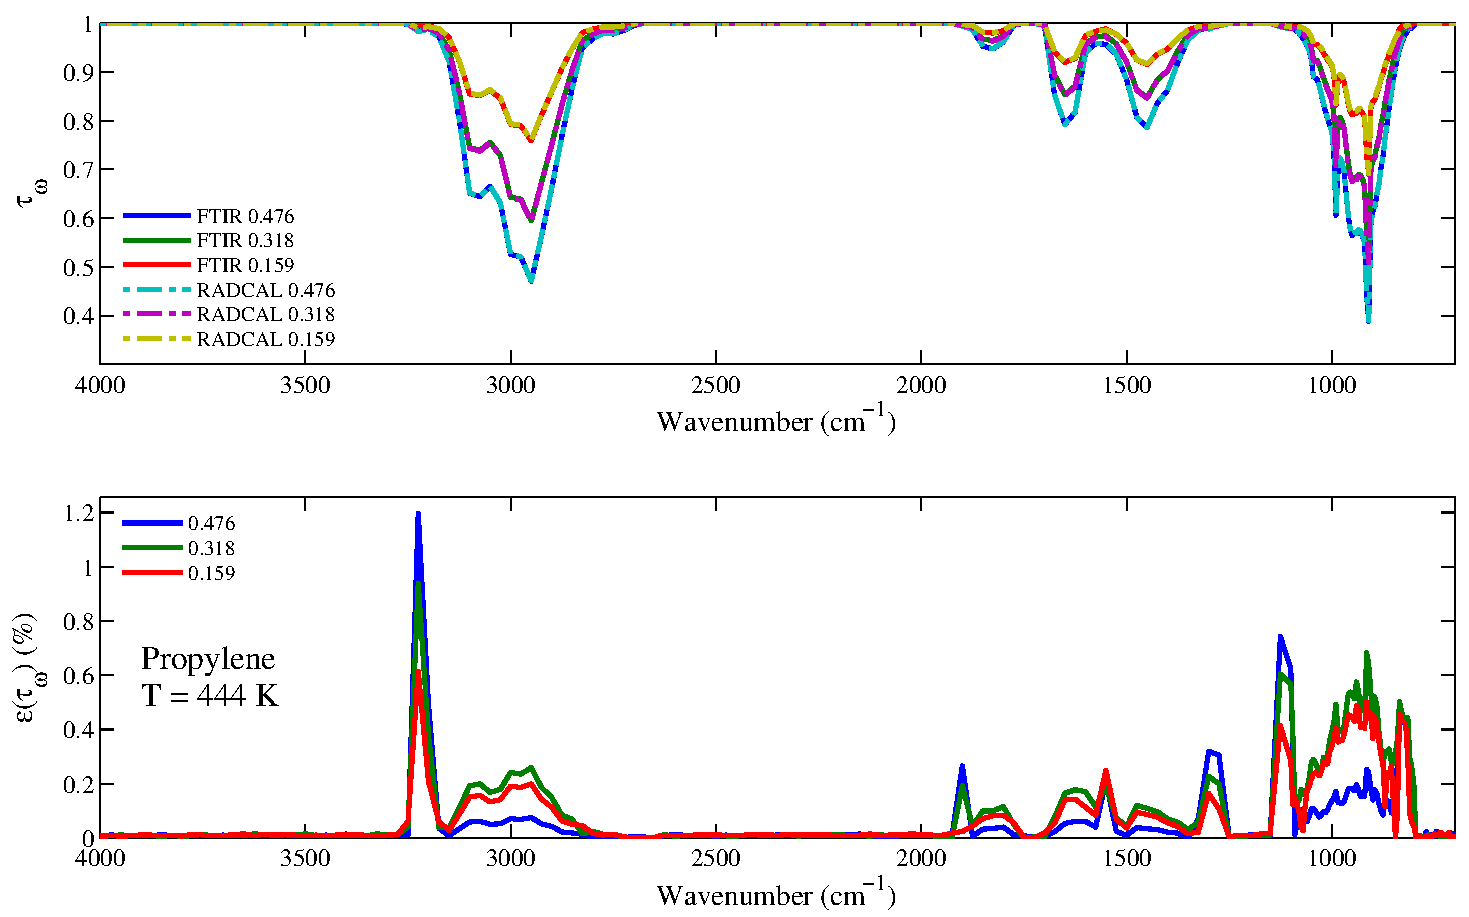
\includegraphics[width=\textwidth]{../Verification/Results_Test2/Propylene_444.pdf}
\caption{Top: comparison between the experimental (solid lines) and RadCal-generated synthetic (dashed lines) spectral transmissivity profiles, denoted $\tau_{\omega}$, of propylene of an isothermal homogeneous column of propylene. Bottom: relative transmissivity error, denoted $\epsilon{(\tau_{\omega})}$, between the experiment and the synthetic profiles presented on the top figure. Three different pressure path lengths are considered: 0.476, 0.318, and 0.159 atm.cm. The gas temperature is set at 444~K and the total pressure is 101 kPa. Note: the experimental data resolution has been changed to match that of the narrow band model. \label{fig:propylene_Verify_444K}}
\end{figure}

\begin{figure}[p]
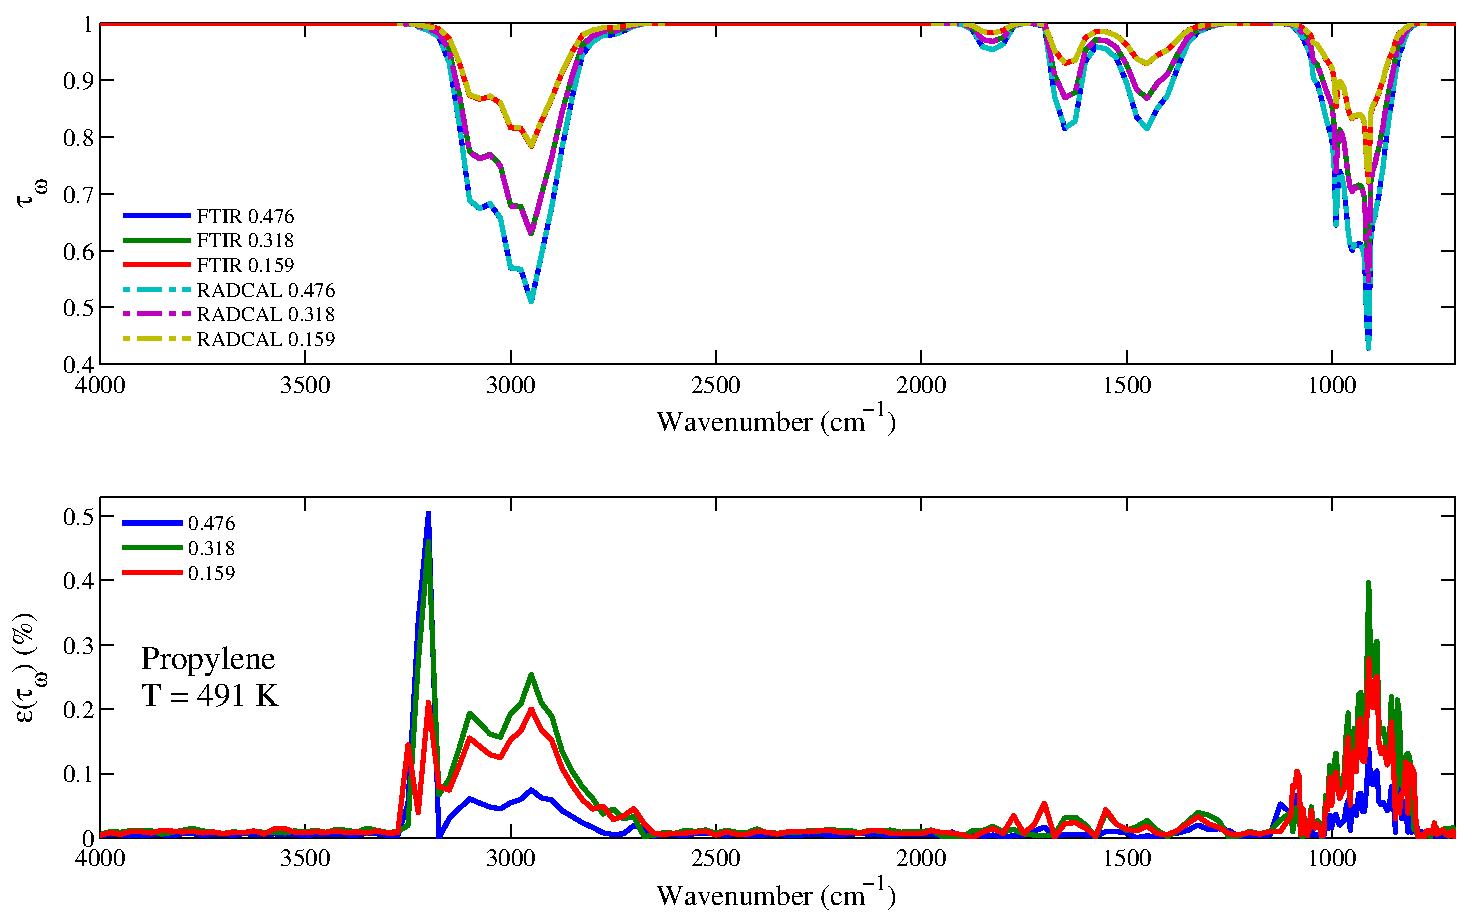
\includegraphics[width=\textwidth]{../Verification/Results_Test2/Propylene_491.pdf}
\caption{Top: comparison between the experimental (solid lines) and RadCal-generated synthetic (dashed lines) spectral transmissivity profiles, denoted $\tau_{\omega}$, of propylene of an isothermal homogeneous column of propylene. Bottom: relative transmissivity error, denoted $\epsilon{(\tau_{\omega})}$, between the experiment and the synthetic profiles presented on the top figure. Three different pressure path lengths are considered: 0.476, 0.318, and 0.159 atm.cm. The gas temperature is set at 491~K and the total pressure is 101 kPa. Note: the experimental data resolution has been changed to match that of the narrow band model. \label{fig:propylene_Verify_491K}}
\end{figure}
\newpage

\begin{figure}[p]
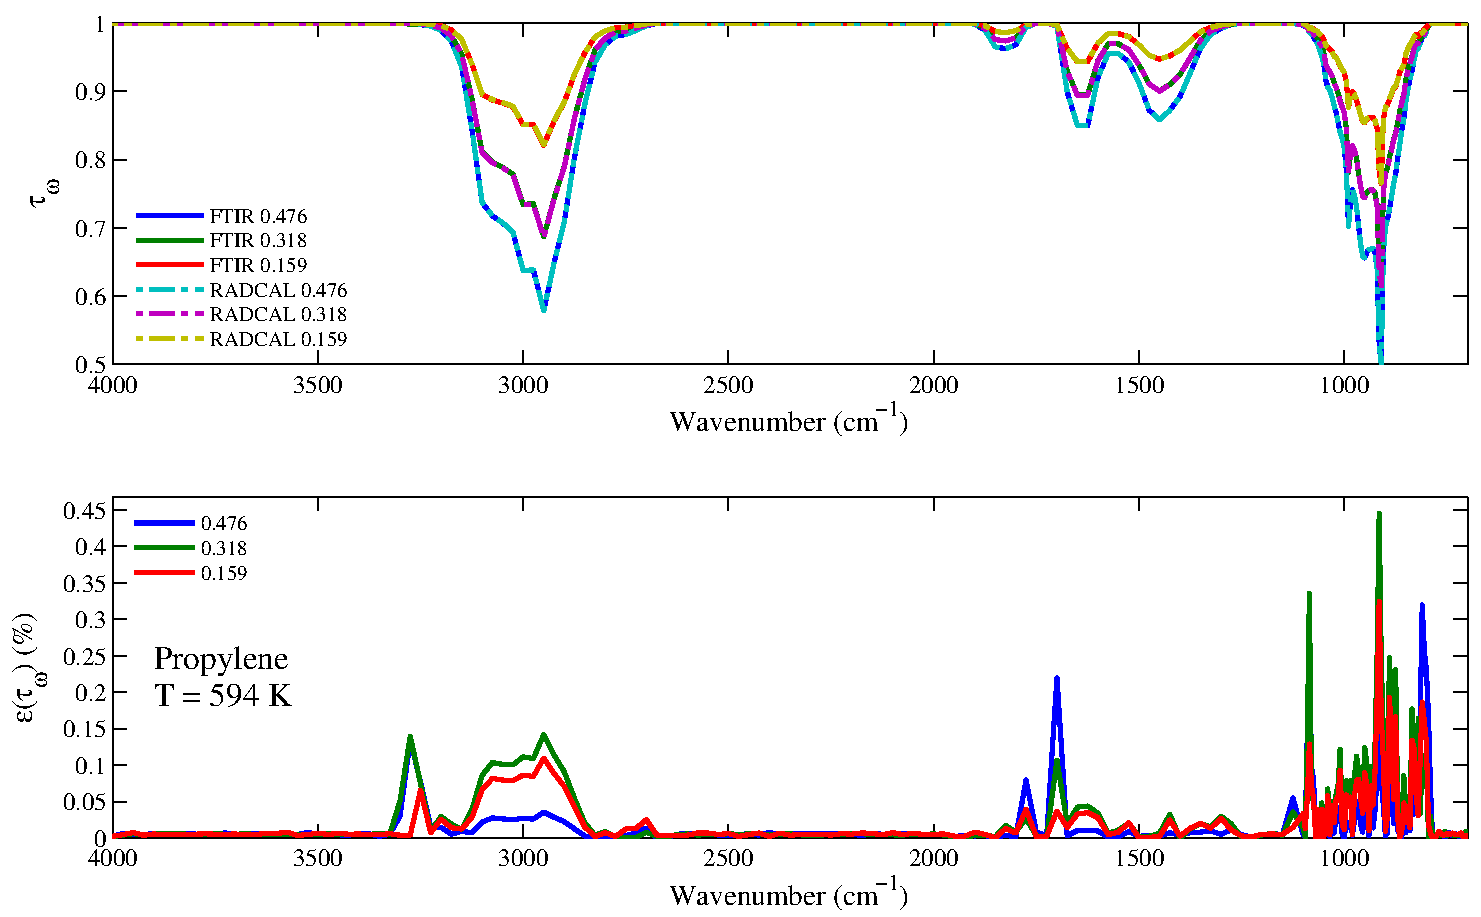
\includegraphics[width=\textwidth]{../Verification/Results_Test2/Propylene_594.pdf}
\caption{Top: comparison between the experimental (solid lines) and RadCal-generated synthetic (dashed lines) spectral transmissivity profiles, denoted $\tau_{\omega}$, of propylene of an isothermal homogeneous column of propylene. Bottom: relative transmissivity error, denoted $\epsilon{(\tau_{\omega})}$, between the experiment and the synthetic profiles presented on the top figure. Three different pressure path lengths are considered: 0.476, 0.318, and 0.159 atm.cm. The gas temperature is set at 594~K and the total pressure is 101 kPa. Note: the experimental data resolution has been changed to match that of the narrow band model. \label{fig:propylene_Verify_594K}}
\end{figure}

\begin{figure}[p]
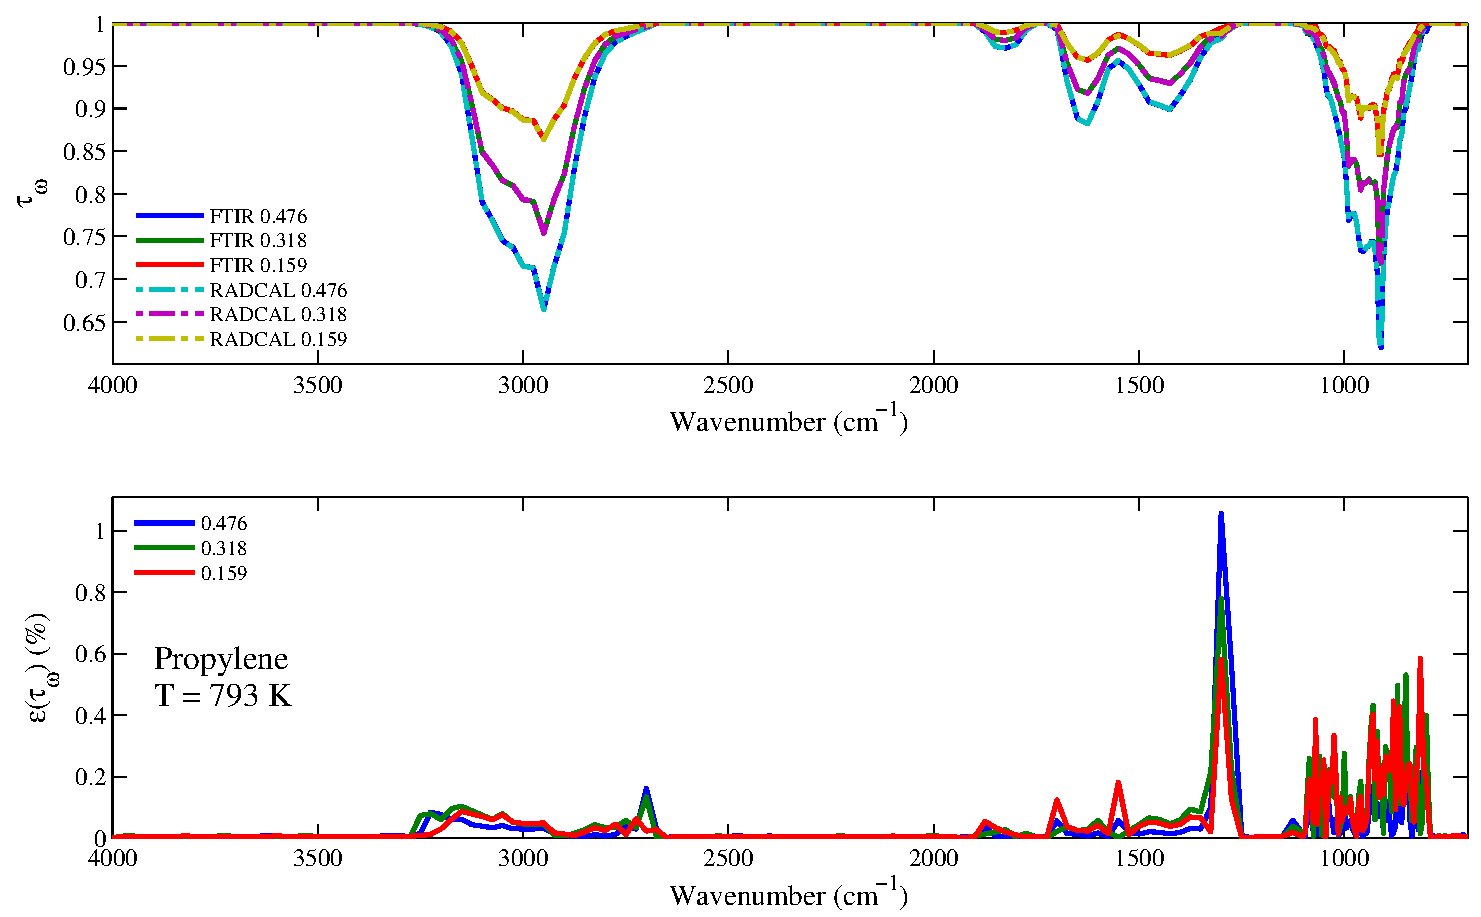
\includegraphics[width=\textwidth]{../Verification/Results_Test2/Propylene_793.pdf}
\caption{Top: comparison between the experimental (solid lines) and RadCal-generated synthetic (dashed lines) spectral transmissivity profiles, denoted $\tau_{\omega}$, of propylene of an isothermal homogeneous column of propylene. Bottom: relative transmissivity error, denoted $\epsilon{(\tau_{\omega})}$, between the experiment and the synthetic profiles presented on the top figure. Three different pressure path lengths are considered: 0.476, 0.318, and 0.159 atm.cm. The gas temperature is set at 793~K and the total pressure is 101 kPa. Note: the experimental data resolution has been changed to match that of the narrow band model. \label{fig:propylene_Verify_793K}}
\end{figure}
\newpage

\begin{figure}[p]
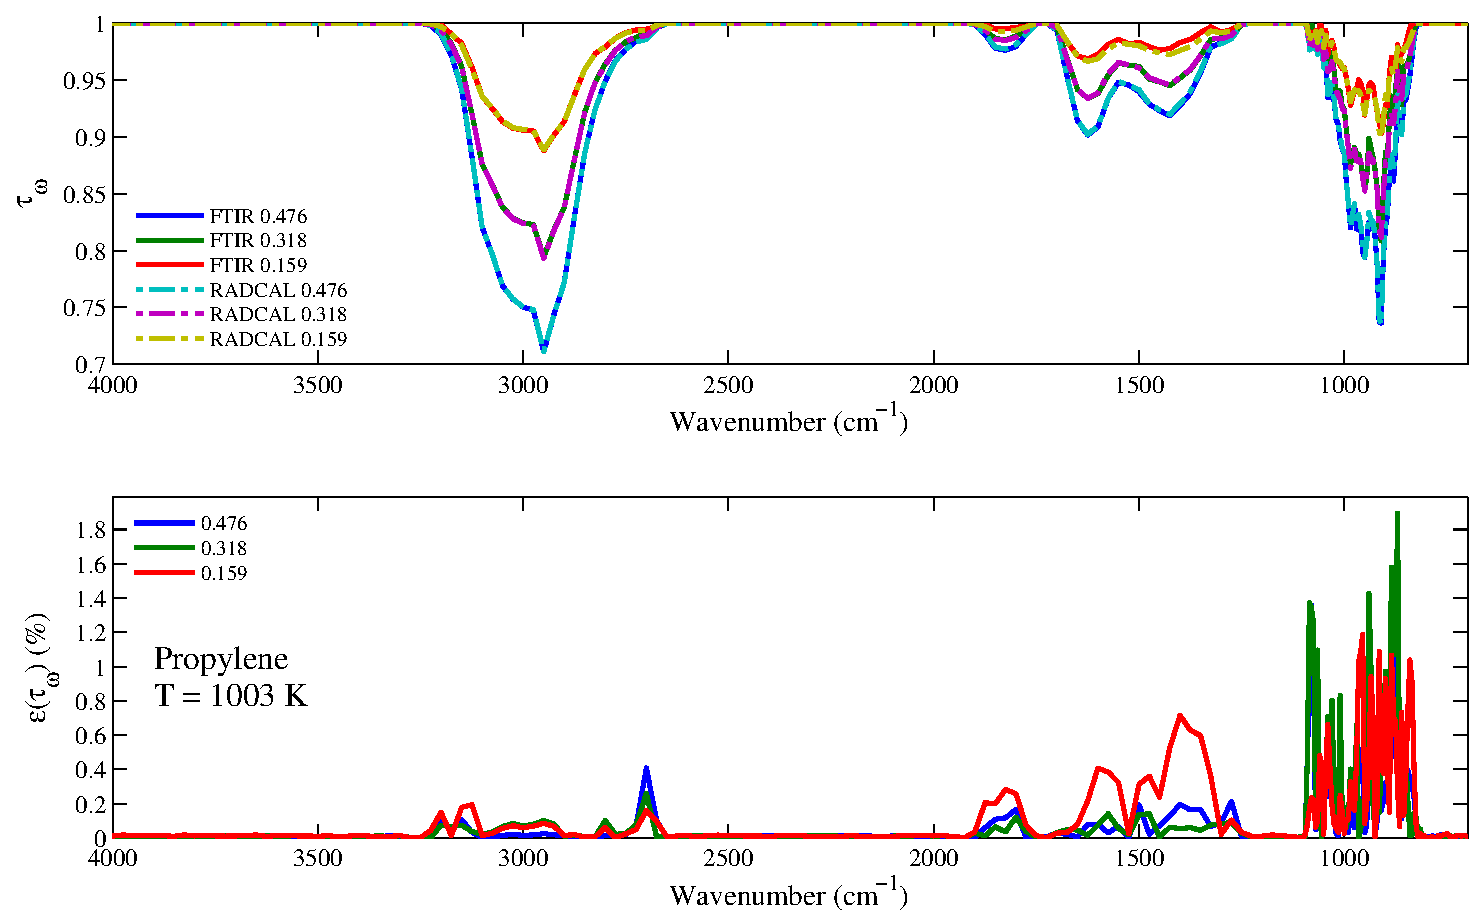
\includegraphics[width=\textwidth]{../Verification/Results_Test2/Propylene_1003.pdf}
\caption{Top: comparison between the experimental (solid lines) and RadCal-generated synthetic (dashed lines) spectral transmissivity profiles, denoted $\tau_{\omega}$, of propylene of an isothermal homogeneous column of propylene. Bottom: relative transmissivity error, denoted $\epsilon{(\tau_{\omega})}$, between the experiment and the synthetic profiles presented on the top figure. Three different pressure path lengths are considered: 0.476, 0.318, and 0.159 atm.cm. The gas temperature is set at 1003~K and the total pressure is 101 kPa. Note: the experimental data resolution has been changed to match that of the narrow band model. \label{fig:propylene_Verify_1003K}}
\end{figure}


\clearpage

\section{Propane: $\rm C_3H_8$}

\begin{figure}[h]
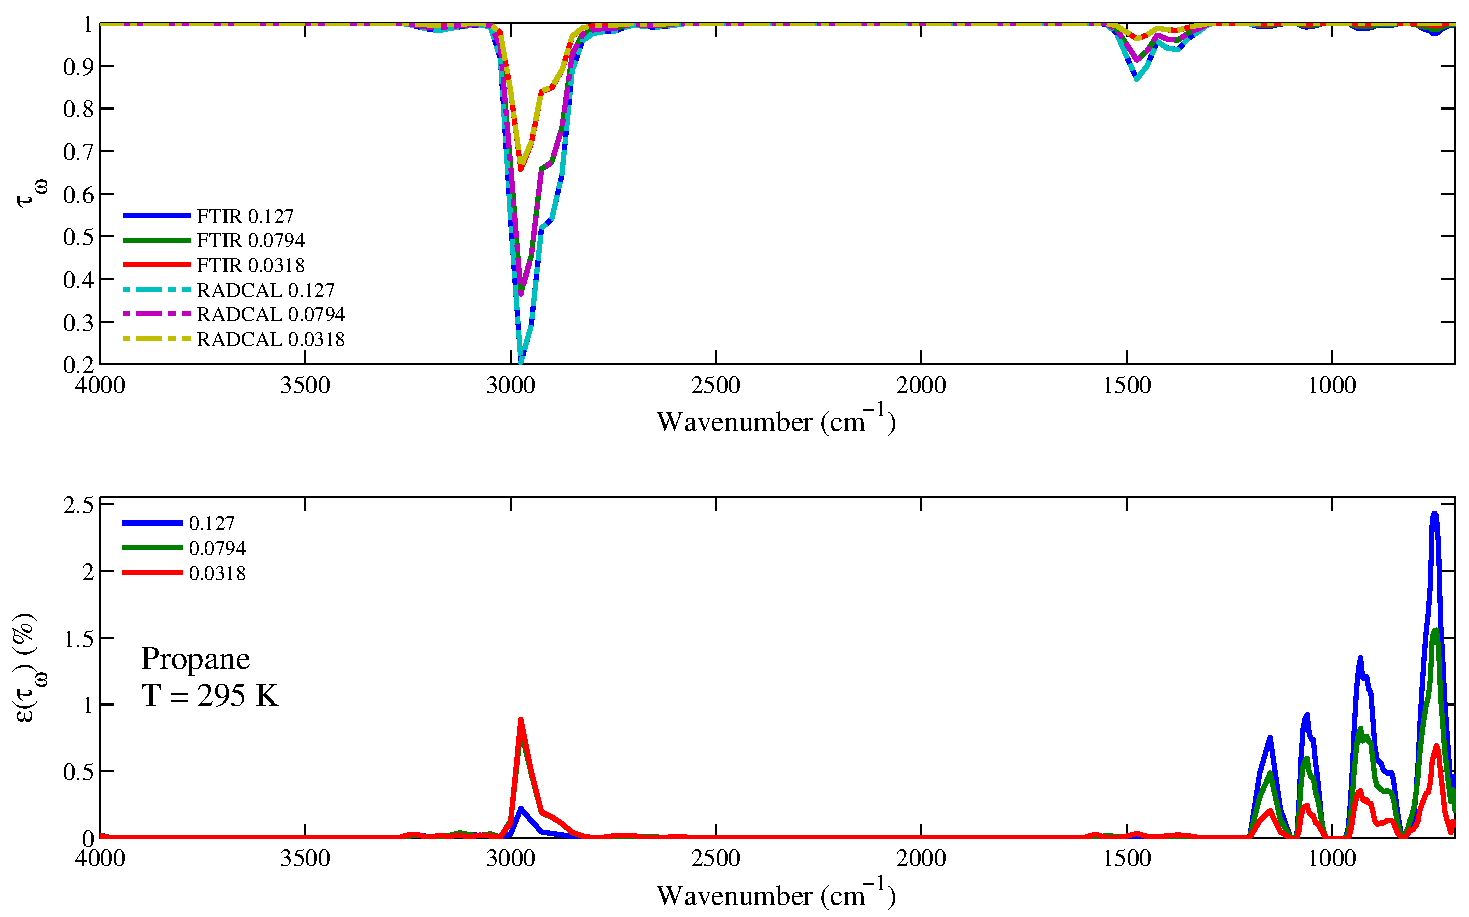
\includegraphics[width=\textwidth]{../Verification/Results_Test2/Propane_295.pdf}
\caption{Top: comparison between the experimental (solid lines) and RadCal-generated synthetic (dashed lines) spectral transmissivity profiles, denoted $\tau_{\omega}$, of propane of an isothermal homogeneous column of propane. Bottom: relative transmissivity error, denoted $\epsilon{(\tau_{\omega})}$, between the experiment and the synthetic profiles presented on the top figure. Three different pressure path lengths are considered: 0.127, 0.0794, and 0.0318 atm.cm. The gas temperature is set at 295~K and the total pressure is 101 kPa. Note: the experimental data resolution has been changed to match that of the narrow band model. \label{fig:propane_Verify_295K}}
\end{figure}

\newpage

\begin{figure}[p]
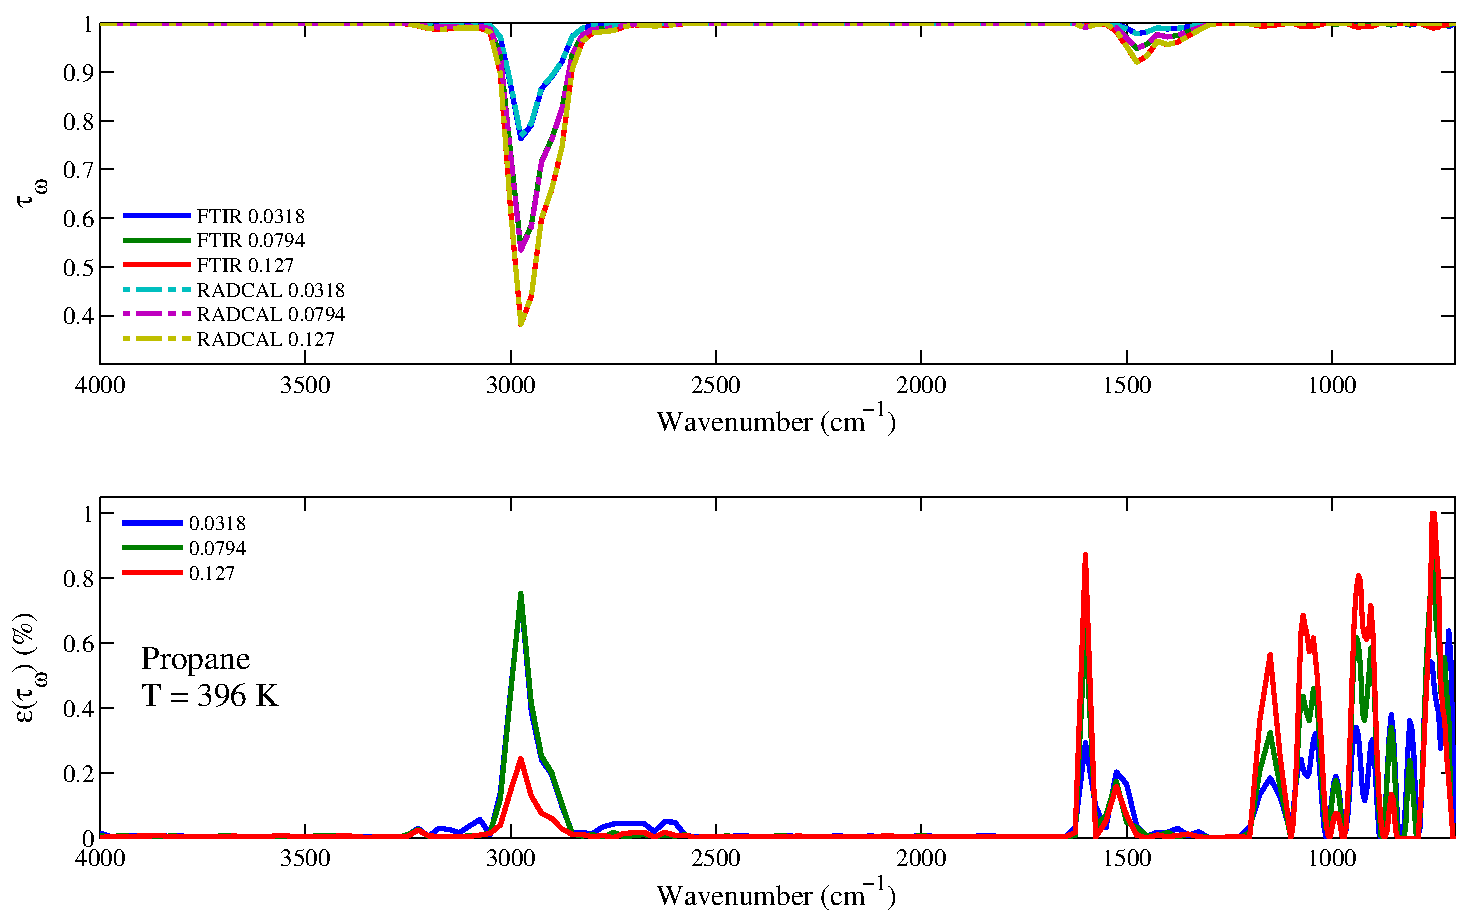
\includegraphics[width=\textwidth]{../Verification/Results_Test2/Propane_396.pdf}
\caption{Top: comparison between the experimental (solid lines) and RadCal-generated synthetic (dashed lines) spectral transmissivity profiles, denoted $\tau_{\omega}$, of propane of an isothermal homogeneous column of propane. Bottom: relative transmissivity error, denoted $\epsilon{(\tau_{\omega})}$, between the experiment and the synthetic profiles presented on the top figure. Three different pressure path lengths are considered: 0.0318, 0.0794, and 0.127 atm.cm. The gas temperature is set at 396~K and the total pressure is 101 kPa. Note: the experimental data resolution has been changed to match that of the narrow band model. \label{fig:propane_Verify_396K}}
\end{figure}
\newpage

\begin{figure}[p]
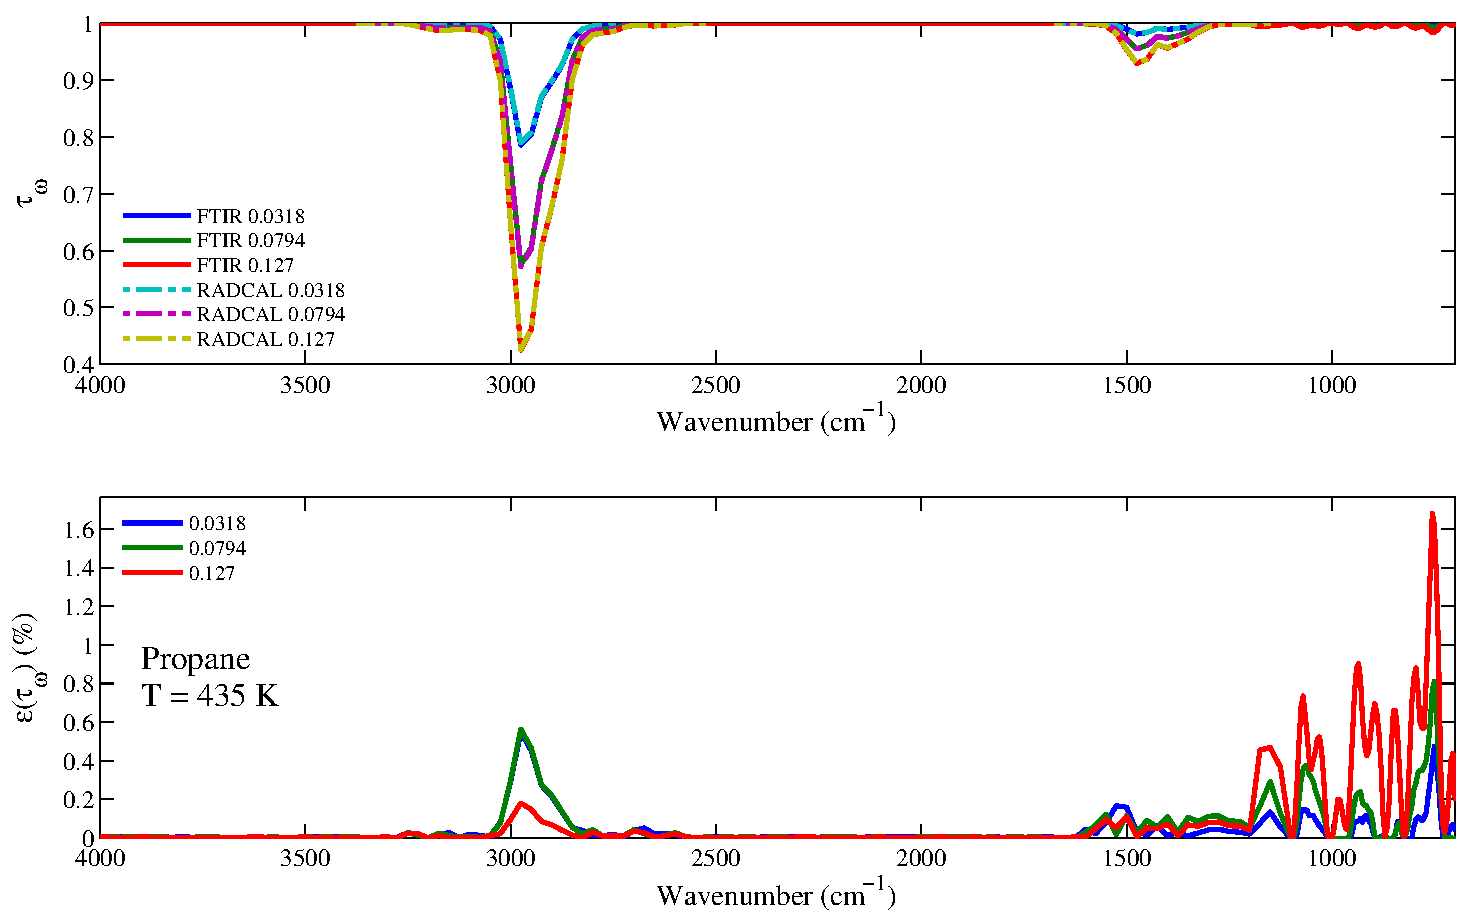
\includegraphics[width=\textwidth]{../Verification/Results_Test2/Propane_435.pdf}
\caption{Top: comparison between the experimental (solid lines) and RadCal-generated synthetic (dashed lines) spectral transmissivity profiles, denoted $\tau_{\omega}$, of propane of an isothermal homogeneous column of propane. Bottom: relative transmissivity error, denoted $\epsilon{(\tau_{\omega})}$, between the experiment and the synthetic profiles presented on the top figure. Three different pressure path lengths are considered: 0.0318, 0.0794, and 0.127 atm.cm. The gas temperature is set at 435~K and the total pressure is 101 kPa. Note: the experimental data resolution has been changed to match that of the narrow band model. \label{fig:propane_Verify_435K}}
\end{figure}

\begin{figure}[p]
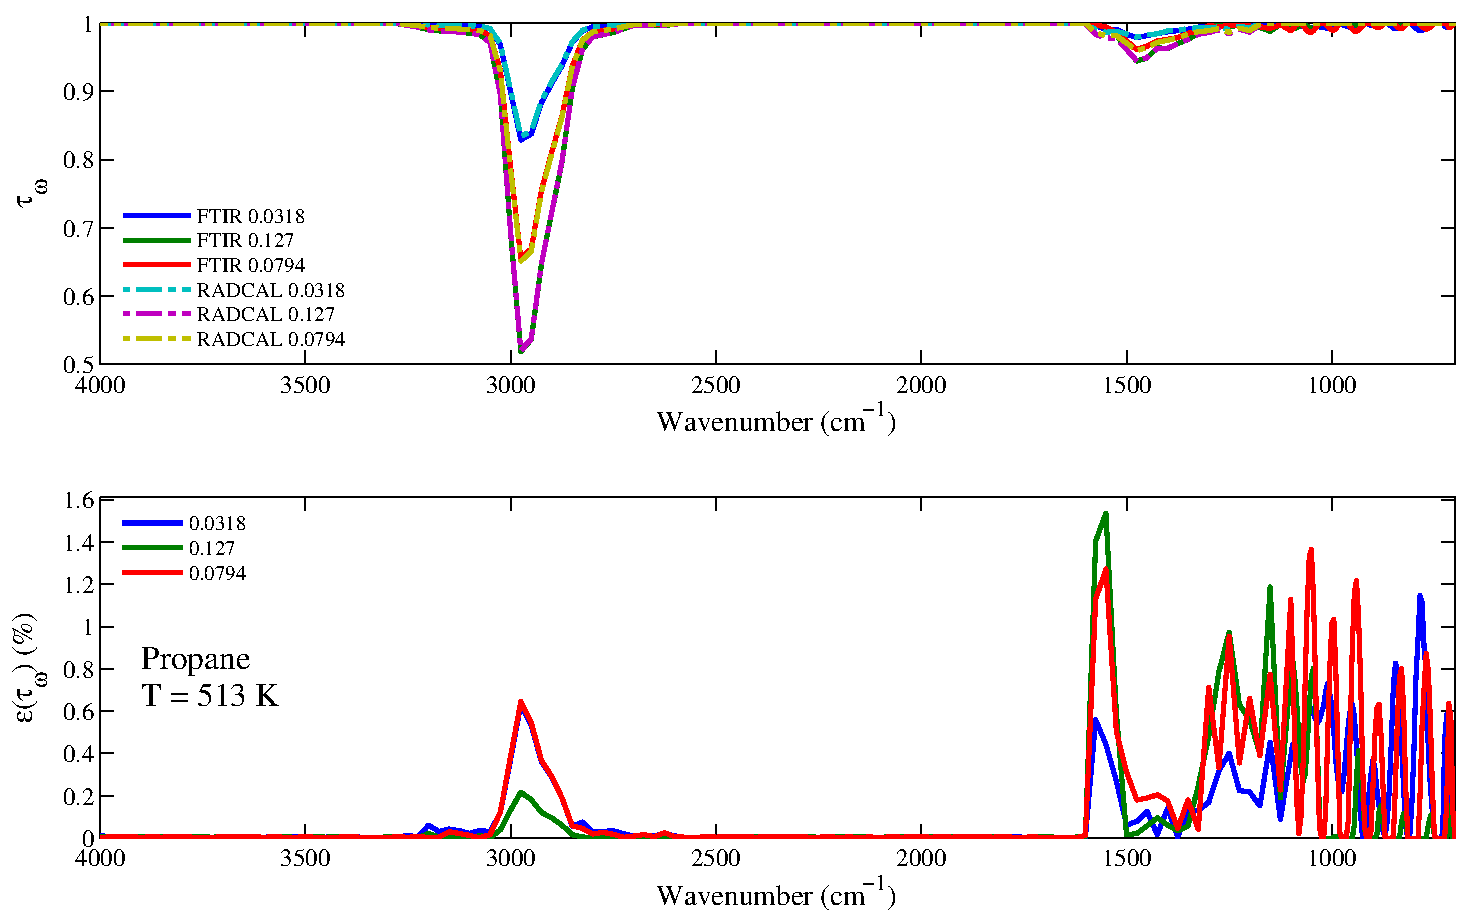
\includegraphics[width=\textwidth]{../Verification/Results_Test2/Propane_513.pdf}
\caption{Top: comparison between the experimental (solid lines) and RadCal-generated synthetic (dashed lines) spectral transmissivity profiles, denoted $\tau_{\omega}$, of propane of an isothermal homogeneous column of propane. Bottom: relative transmissivity error, denoted $\epsilon{(\tau_{\omega})}$, between the experiment and the synthetic profiles presented on the top figure. Three different pressure path lengths are considered: 0.0318, 0.127, and 0.0794 atm.cm. The gas temperature is set at 513~K and the total pressure is 101 kPa. Note: the experimental data resolution has been changed to match that of the narrow band model. \label{fig:propane_Verify_513K}}
\end{figure}

\begin{figure}[p]
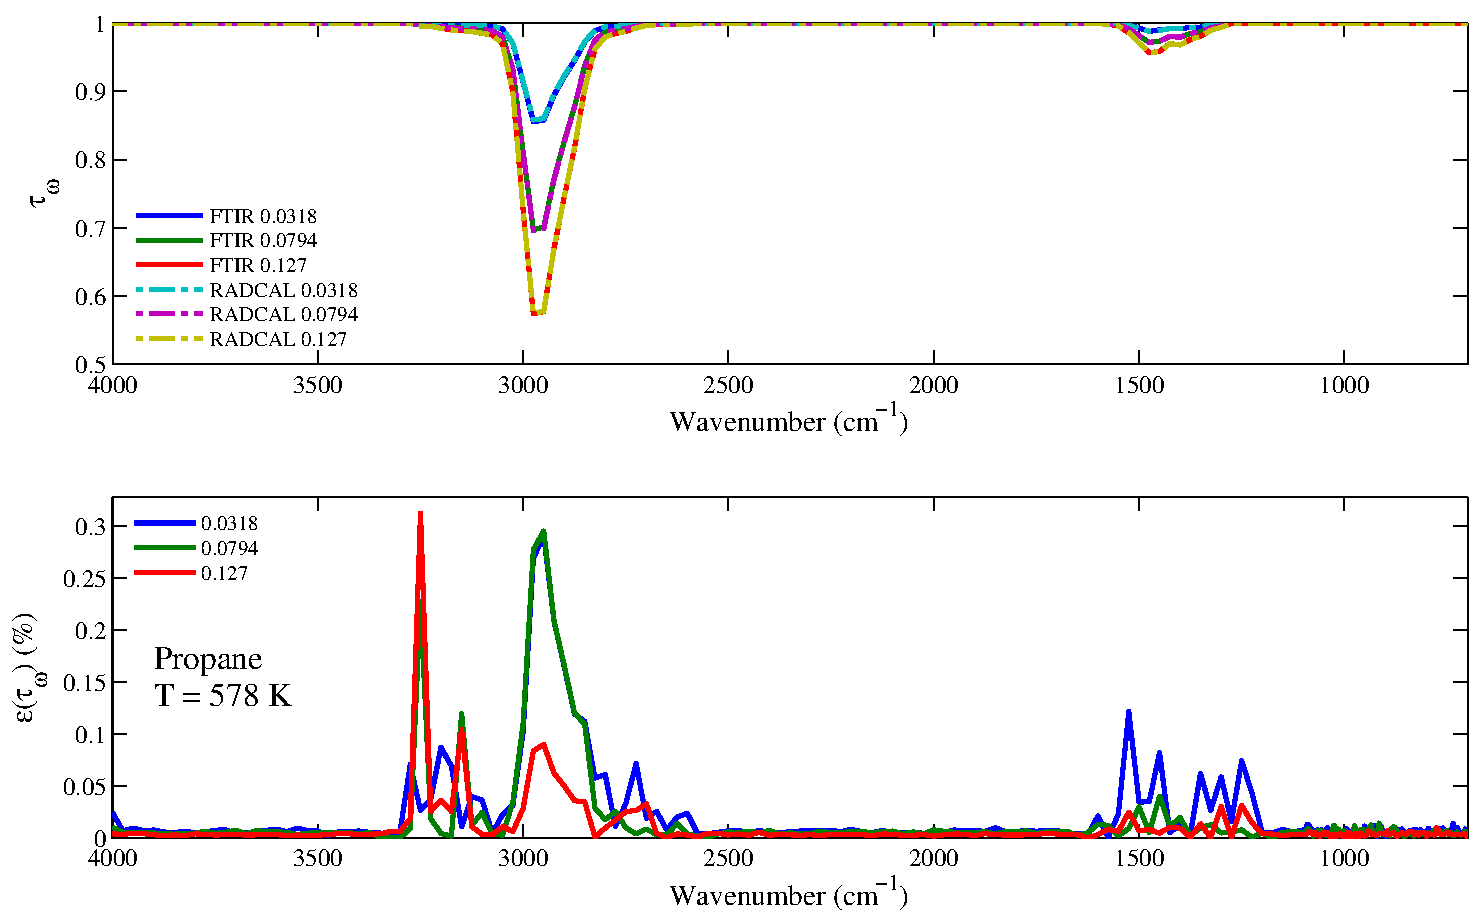
\includegraphics[width=\textwidth]{../Verification/Results_Test2/Propane_578.pdf}
\caption{Top: comparison between the experimental (solid lines) and RadCal-generated synthetic (dashed lines) spectral transmissivity profiles, denoted $\tau_{\omega}$, of propane of an isothermal homogeneous column of propane. Bottom: relative transmissivity error, denoted $\epsilon{(\tau_{\omega})}$, between the experiment and the synthetic profiles presented on the top figure. Three different pressure path lengths are considered: 0.0318, 0.0794, and 0.127 atm.cm. The gas temperature is set at 578~K and the total pressure is 101 kPa. Note: the experimental data resolution has been changed to match that of the narrow band model. \label{fig:propane_Verify_578K}}
\end{figure}

\begin{figure}[p]
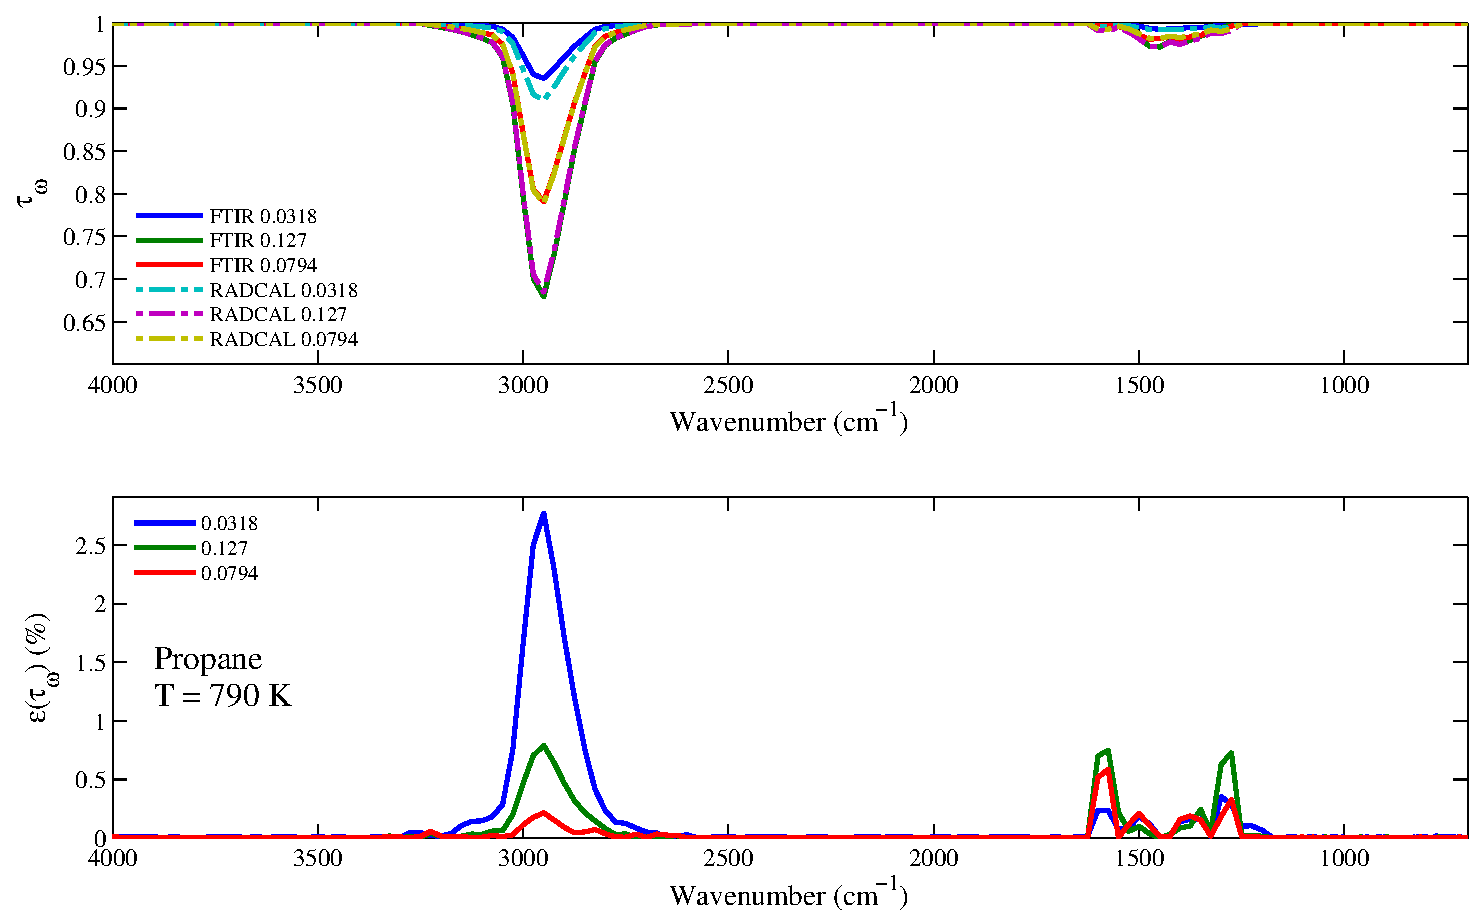
\includegraphics[width=\textwidth]{../Verification/Results_Test2/Propane_790.pdf}
\caption{Top: comparison between the experimental (solid lines) and RadCal-generated synthetic (dashed lines) spectral transmissivity profiles, denoted $\tau_{\omega}$, of propane of an isothermal homogeneous column of propane. Bottom: relative transmissivity error, denoted $\epsilon{(\tau_{\omega})}$, between the experiment and the synthetic profiles presented on the top figure. Three different pressure path lengths are considered: 0.0318, 0.0794, and 0.127 atm.cm. The gas temperature is set at 790~K and the total pressure is 101 kPa. Note: the experimental data resolution has been changed to match that of the narrow band model. \label{fig:propane_Verify_790K}}
\end{figure}

\begin{figure}[p]
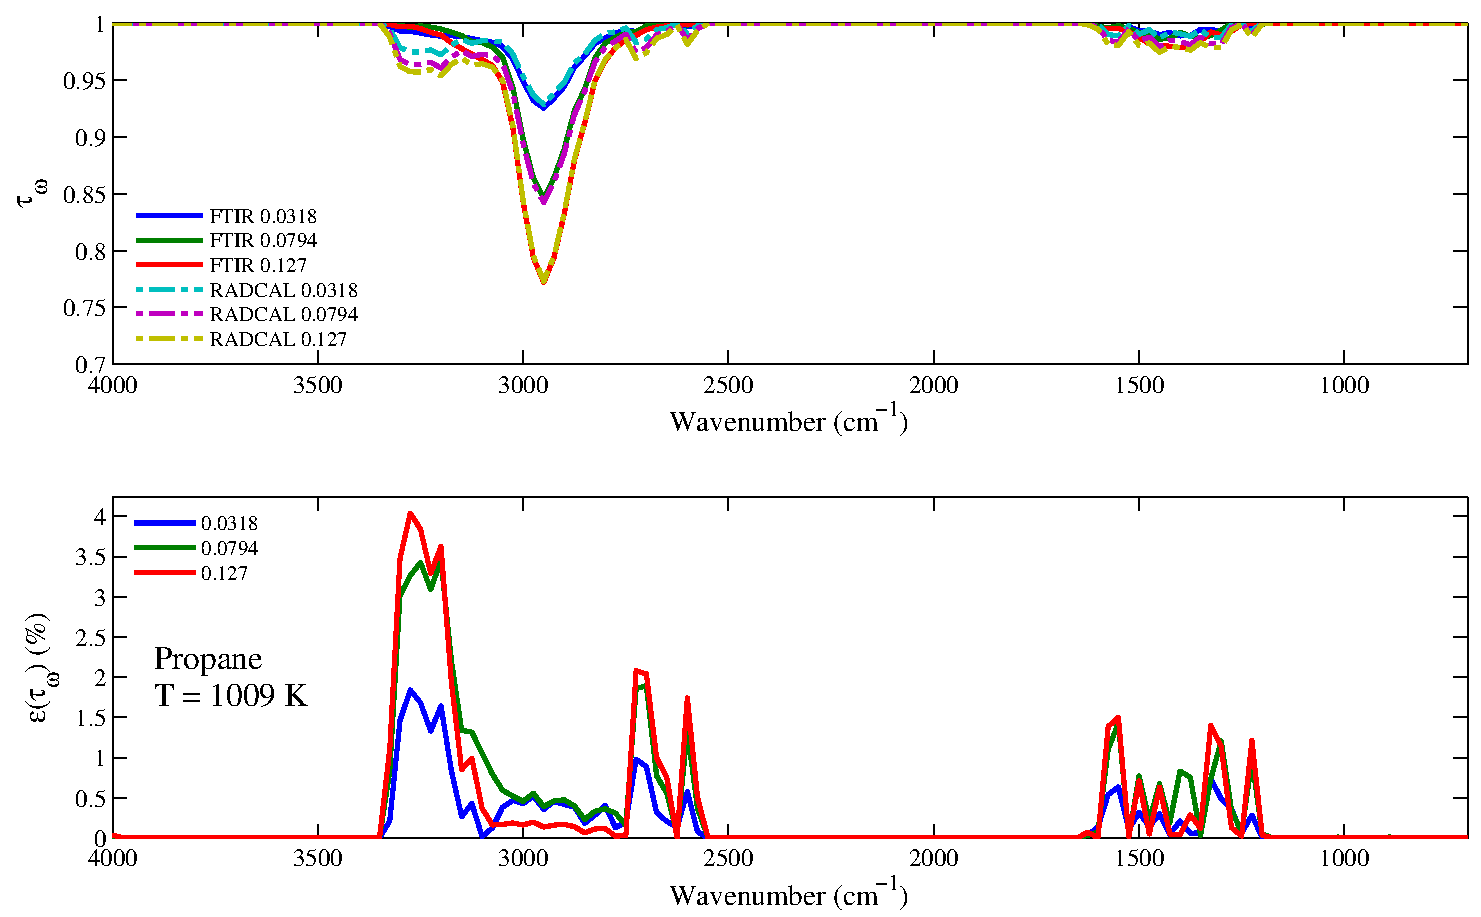
\includegraphics[width=\textwidth]{../Verification/Results_Test2/Propane_1009.pdf}
\caption{Top: comparison between the experimental (solid lines) and RadCal-generated synthetic (dashed lines) spectral transmissivity profiles, denoted $\tau_{\omega}$, of propane of an isothermal homogeneous column of propane. Bottom: relative transmissivity error, denoted $\epsilon{(\tau_{\omega})}$, between the experiment and the synthetic profiles presented on the top figure. Three different pressure path lengths are considered: 0.0318, 0.0794, and 0.127 atm.cm. The gas temperature is set at 1009~K and the total pressure is 101 kPa. Note: the experimental data resolution has been changed to match that of the narrow band model. \label{fig:propane_Verify_1009K}}
\end{figure}


\clearpage

\section{Toluene: $\rm C_7H_8$}

\begin{figure}[h]
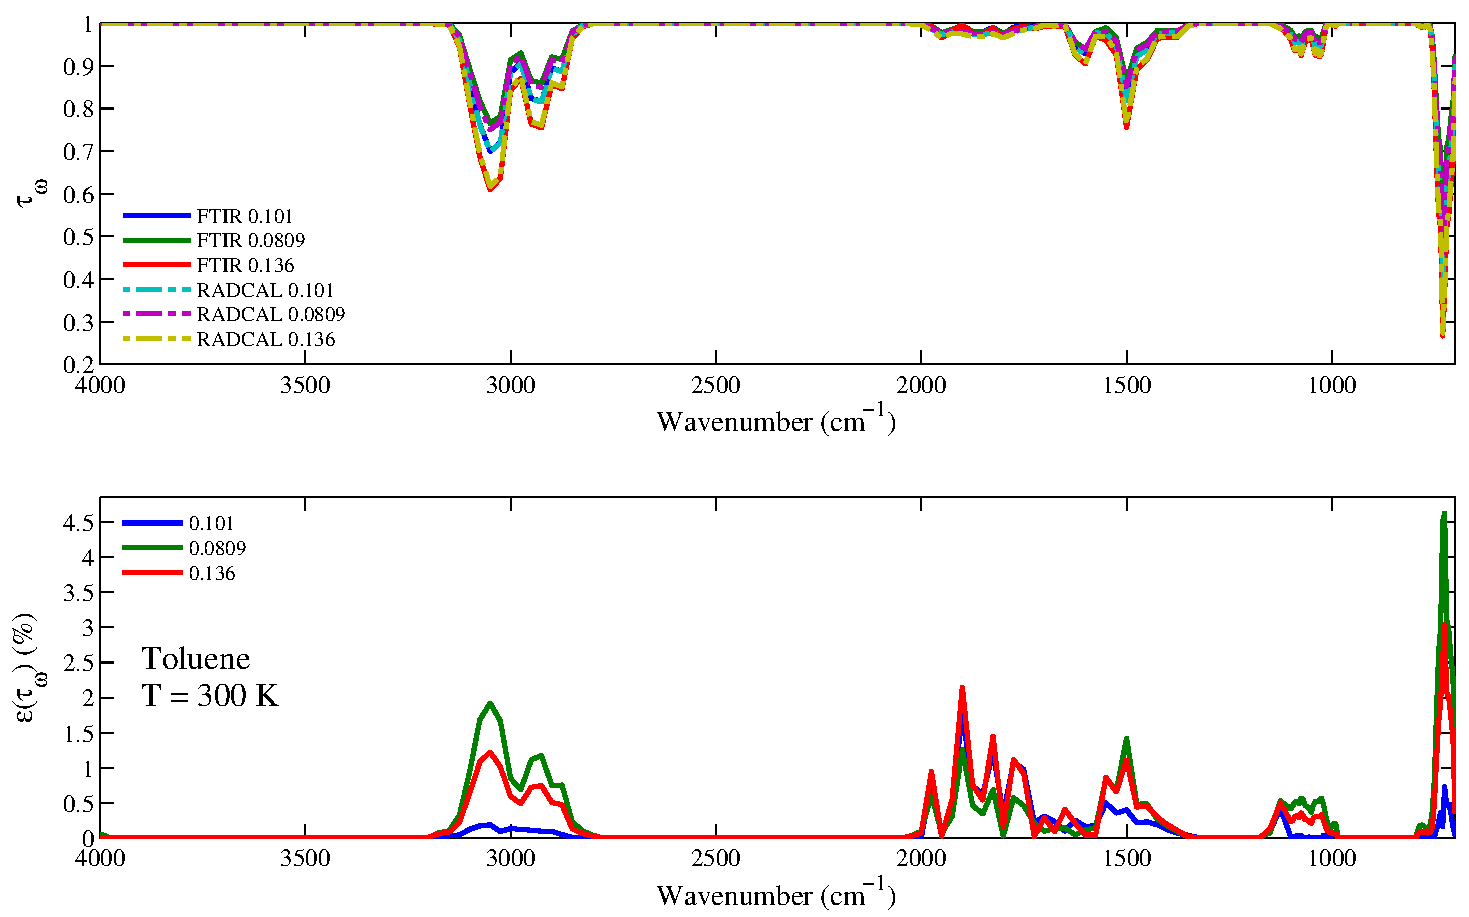
\includegraphics[width=\textwidth]{../Verification/Results_Test2/Toluene_300.pdf}
\caption{Top: comparison between the experimental (solid lines) and RadCal-generated synthetic (dashed lines) spectral transmissivity profiles, denoted $\tau_{\omega}$, of toluene of an isothermal homogeneous column of toluene. Bottom: relative transmissivity error, denoted $\epsilon{(\tau_{\omega})}$, between the experiment and the synthetic profiles presented on the top figure. Three different pressure path lengths are considered: 0.101, 0.0809, and 0.136 atm.cm. The gas temperature is set at 300~K and the total pressure is 101 kPa. Note: the experimental data resolution has been changed to match that of the narrow band model. \label{fig:toluene_Verify_300K}}
\end{figure}

\newpage

\begin{figure}[p]
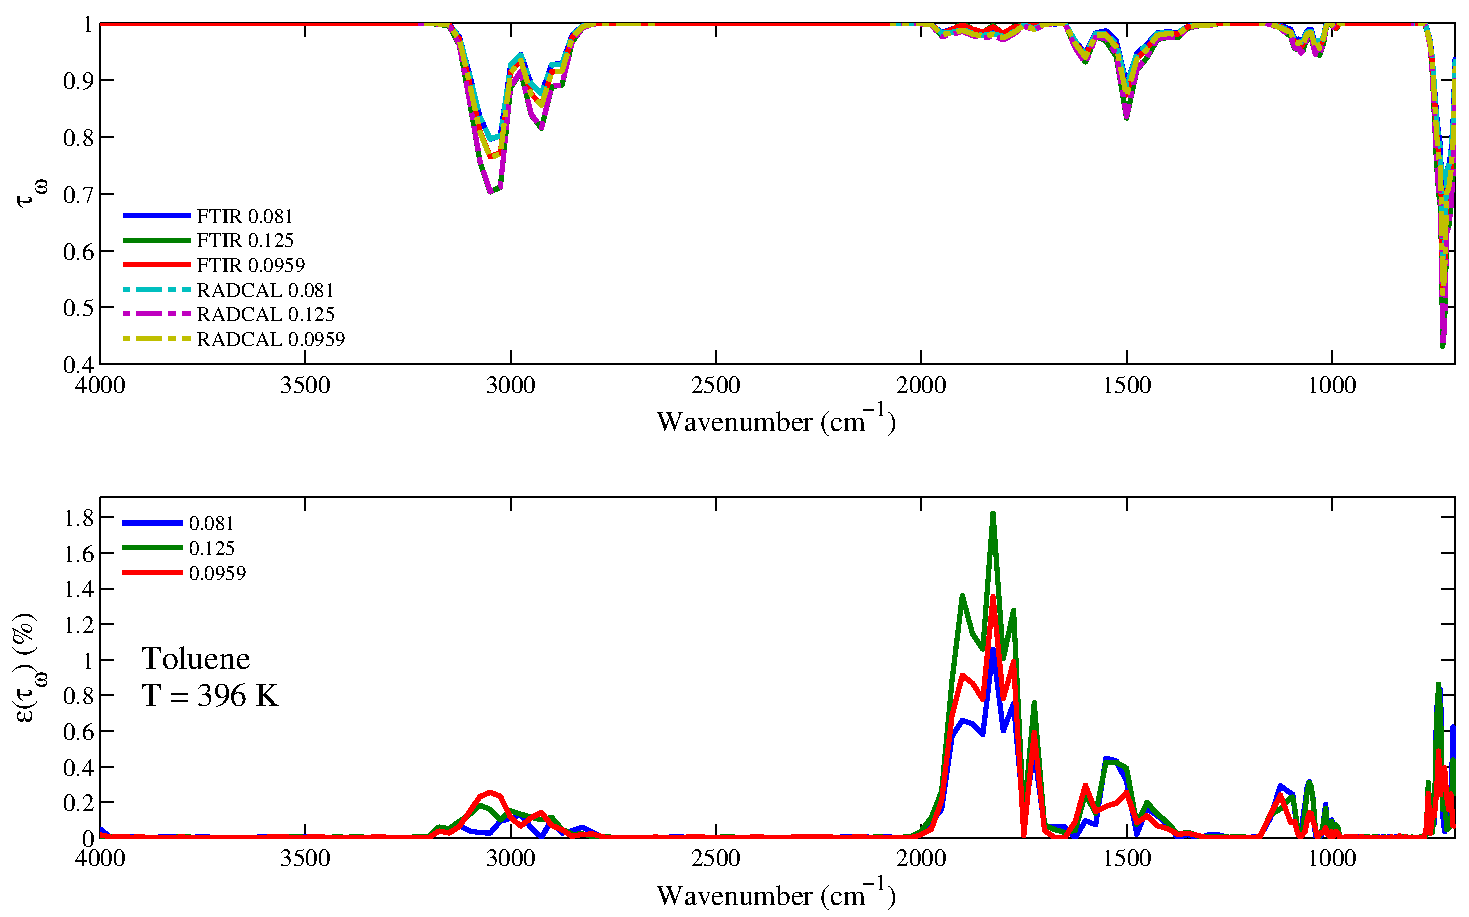
\includegraphics[width=\textwidth]{../Verification/Results_Test2/Toluene_396.pdf}
\caption{Top: comparison between the experimental (solid lines) and RadCal-generated synthetic (dashed lines) spectral transmissivity profiles, denoted $\tau_{\omega}$, of toluene of an isothermal homogeneous column of toluene. Bottom: relative transmissivity error, denoted $\epsilon{(\tau_{\omega})}$, between the experiment and the synthetic profiles presented on the top figure. Three different pressure path lengths are considered: 0.081, 0.125, and 0.0959 atm.cm. The gas temperature is set at 396~K and the total pressure is 101 kPa. Note: the experimental data resolution has been changed to match that of the narrow band model. \label{fig:toluene_Verify_396K}}
\end{figure}

\begin{figure}[p]
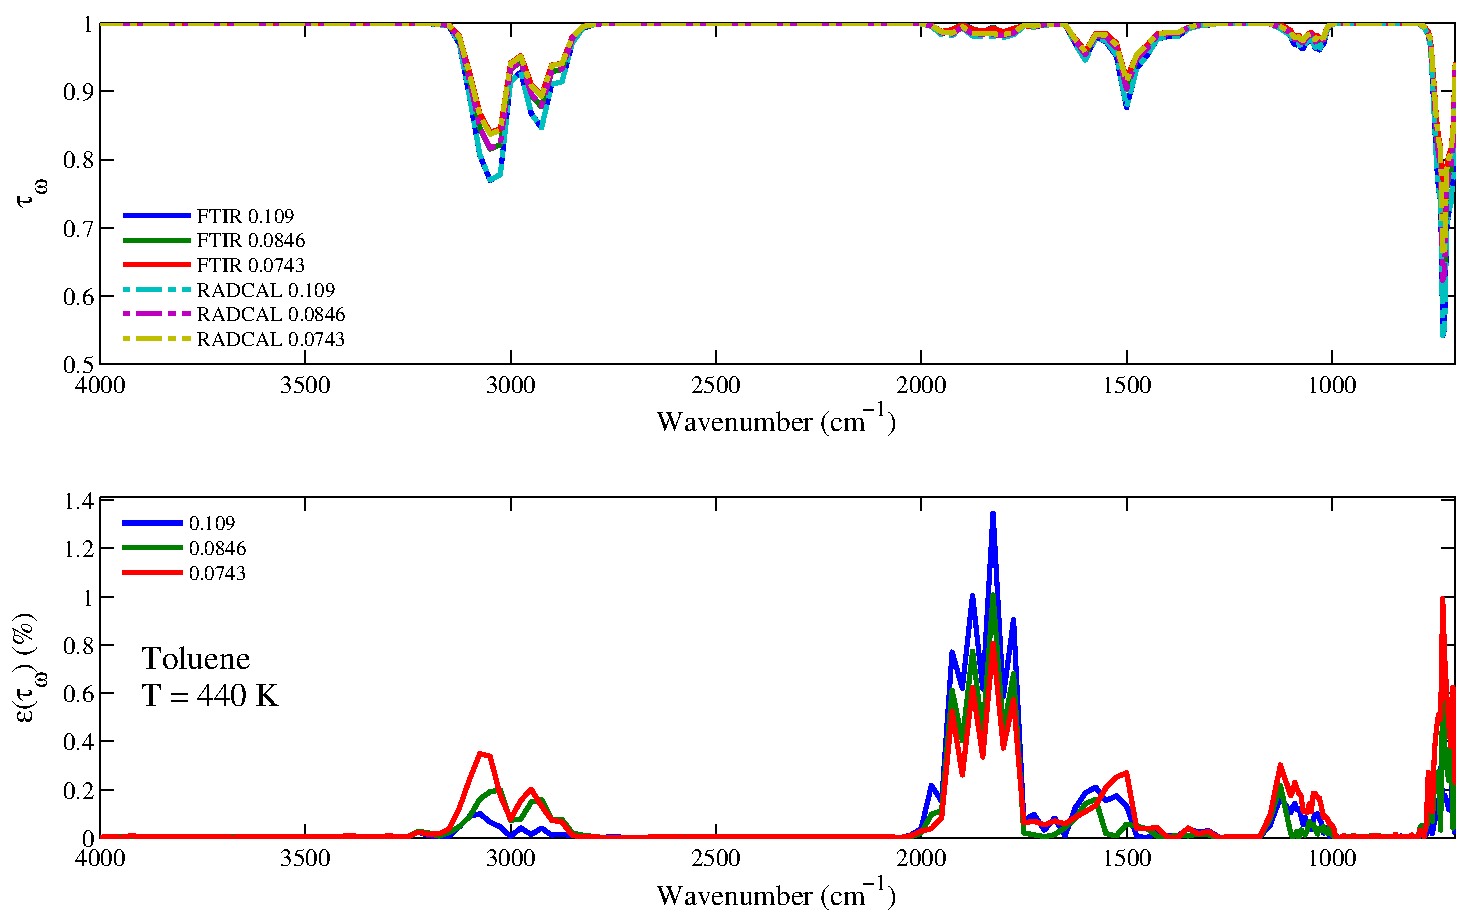
\includegraphics[width=\textwidth]{../Verification/Results_Test2/Toluene_440.pdf}
\caption{Top: comparison between the experimental (solid lines) and RadCal-generated synthetic (dashed lines) spectral transmissivity profiles, denoted $\tau_{\omega}$, of toluene of an isothermal homogeneous column of toluene. Bottom: relative transmissivity error, denoted $\epsilon{(\tau_{\omega})}$, between the experiment and the synthetic profiles presented on the top figure. Three different pressure path lengths are considered: 0.109, 0.0846, and 0.0743 atm.cm. The gas temperature is set at 440~K and the total pressure is 101 kPa. Note: the experimental data resolution has been changed to match that of the narrow band model. \label{fig:toluene_Verify_440K}}
\end{figure}

\begin{figure}[p]
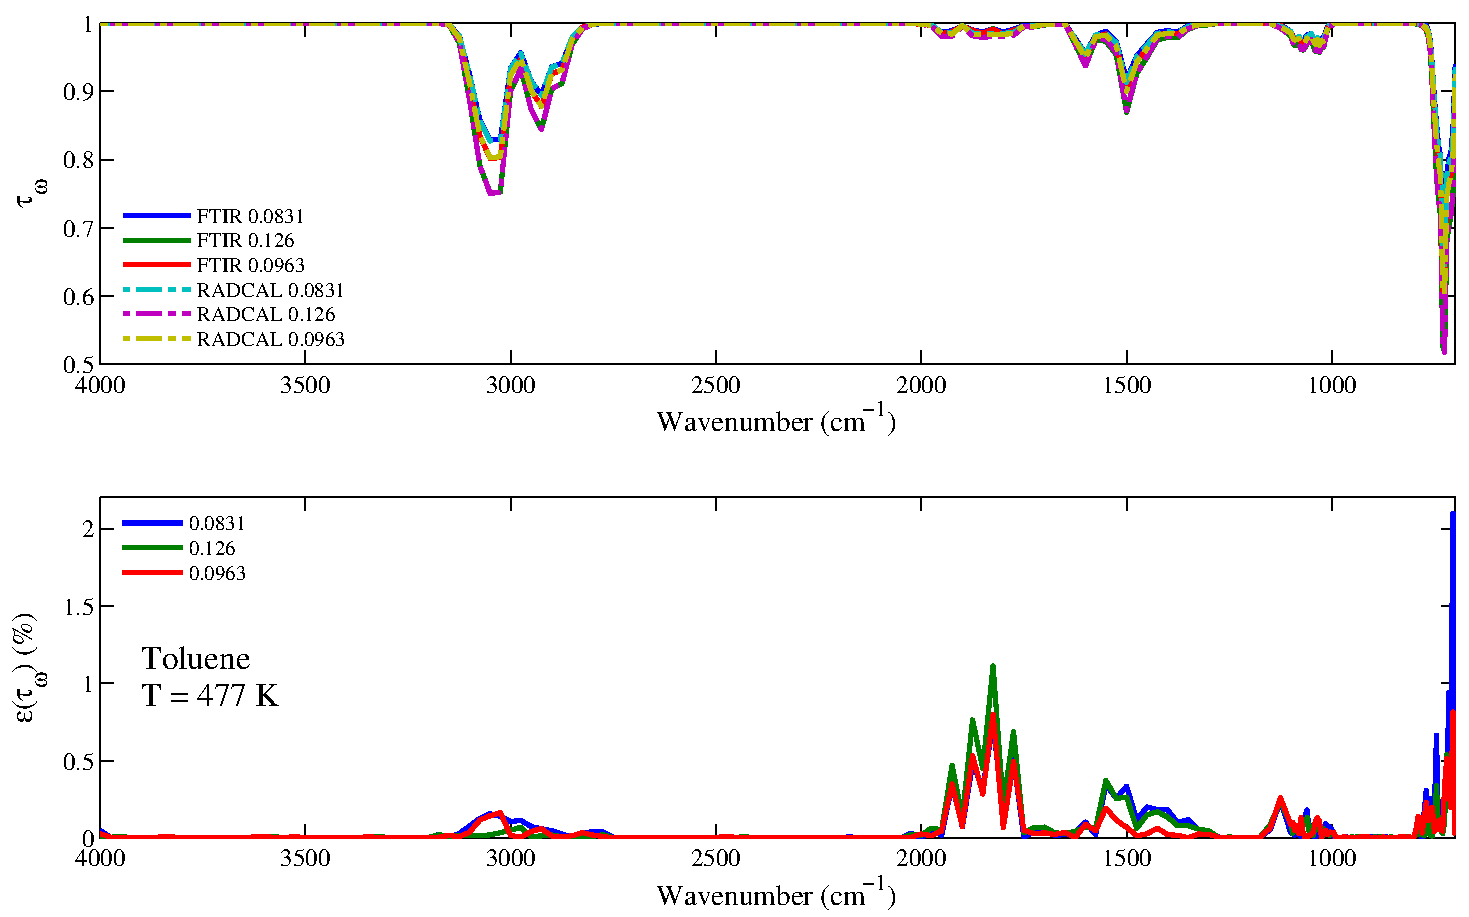
\includegraphics[width=\textwidth]{../Verification/Results_Test2/Toluene_477.pdf}
\caption{Top: comparison between the experimental (solid lines) and RadCal-generated synthetic (dashed lines) spectral transmissivity profiles, denoted $\tau_{\omega}$, of toluene of an isothermal homogeneous column of toluene. Bottom: relative transmissivity error, denoted $\epsilon{(\tau_{\omega})}$, between the experiment and the synthetic profiles presented on the top figure. Three different pressure path lengths are considered: 0.0831, 0.126, and 0.0963 atm.cm. The gas temperature is set at 477~K and the total pressure is 101 kPa. Note: the experimental data resolution has been changed to match that of the narrow band model. \label{fig:toluene_Verify_477K}}
\end{figure}

\begin{figure}[p]
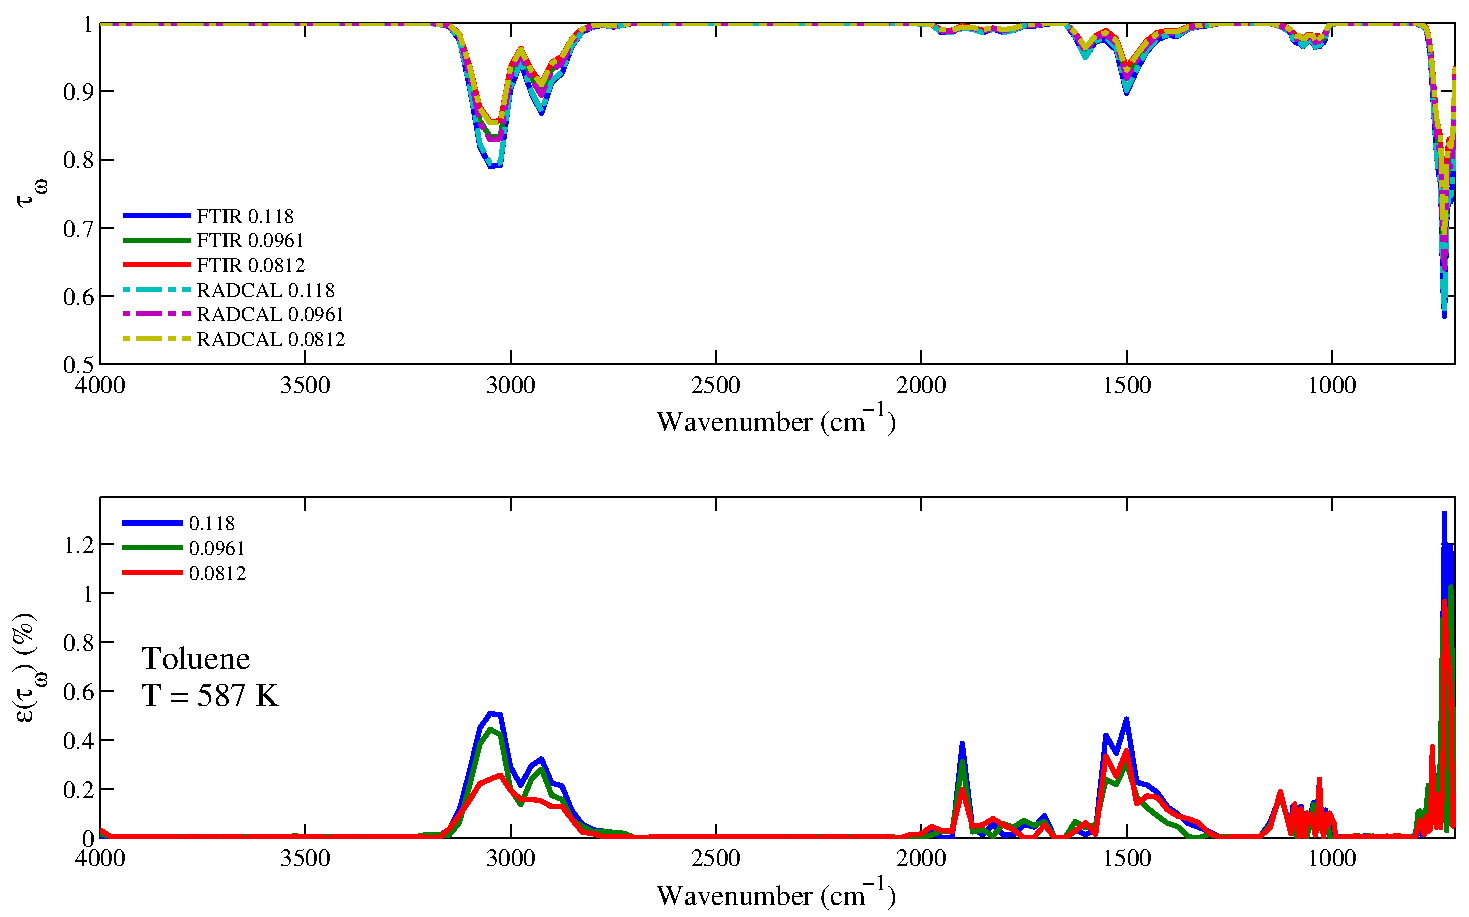
\includegraphics[width=\textwidth]{../Verification/Results_Test2/Toluene_587.pdf}
\caption{Top: comparison between the experimental (solid lines) and RadCal-generated synthetic (dashed lines) spectral transmissivity profiles, denoted $\tau_{\omega}$, of toluene of an isothermal homogeneous column of toluene. Bottom: relative transmissivity error, denoted $\epsilon{(\tau_{\omega})}$, between the experiment and the synthetic profiles presented on the top figure. Three different pressure path lengths are considered: 0.118, 0.0961, and 0.0812 atm.cm. The gas temperature is set at 587~K and the total pressure is 101 kPa. Note: the experimental data resolution has been changed to match that of the narrow band model. \label{fig:toluene_Verify_587K}}
\end{figure}

\begin{figure}[p]
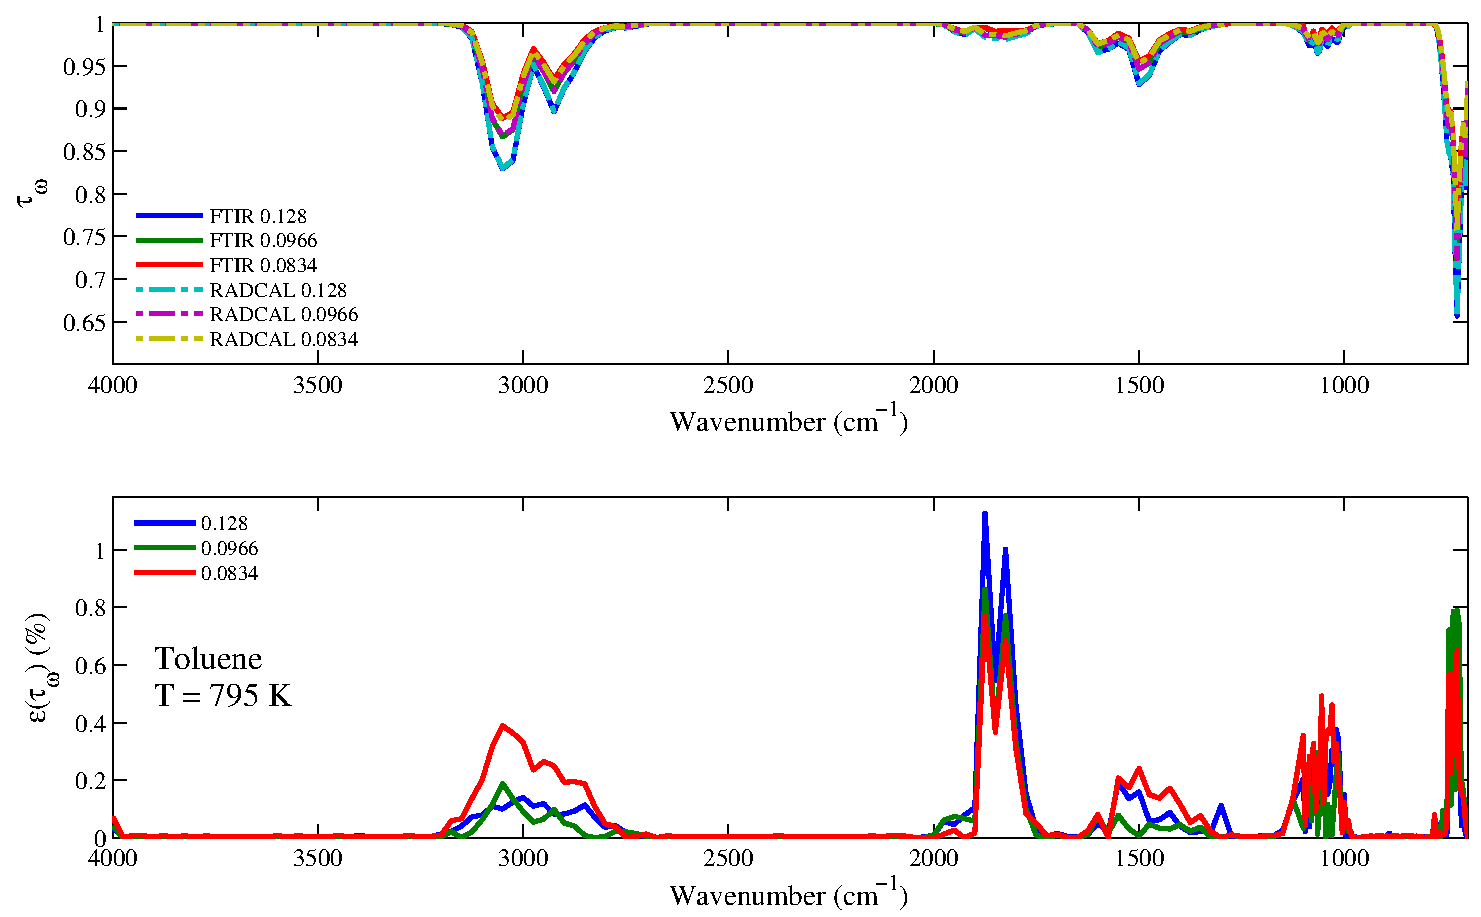
\includegraphics[width=\textwidth]{../Verification/Results_Test2/Toluene_795.pdf}
\caption{Top: comparison between the experimental (solid lines) and RadCal-generated synthetic (dashed lines) spectral transmissivity profiles, denoted $\tau_{\omega}$, of toluene of an isothermal homogeneous column of toluene. Bottom: relative transmissivity error, denoted $\epsilon{(\tau_{\omega})}$, between the experiment and the synthetic profiles presented on the top figure. Three different pressure path lengths are considered: 0.128, 0.0966, and 0.0834 atm.cm. The gas temperature is set at 795~K and the total pressure is 101 kPa. Note: the experimental data resolution has been changed to match that of the narrow band model. \label{fig:toluene_Verify_795K}}
\end{figure}

\begin{figure}[p]
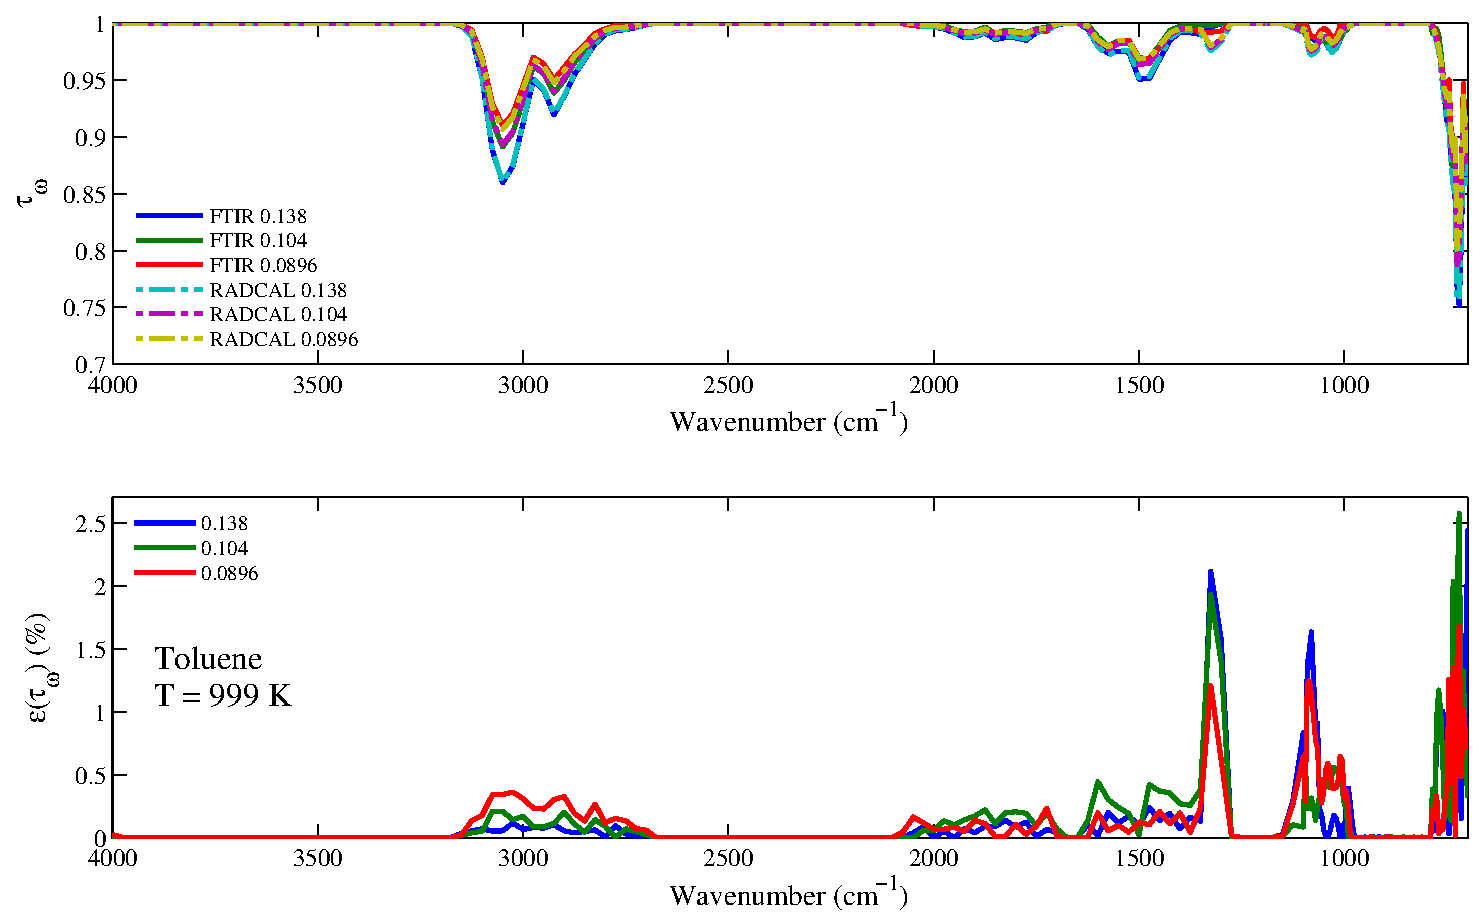
\includegraphics[width=\textwidth]{../Verification/Results_Test2/Toluene_999.pdf}
\caption{Top: comparison between the experimental (solid lines) and RadCal-generated synthetic (dashed lines) spectral transmissivity profiles, denoted $\tau_{\omega}$, of toluene of an isothermal homogeneous column of toluene. Bottom: relative transmissivity error, denoted $\epsilon{(\tau_{\omega})}$, between the experiment and the synthetic profiles presented on the top figure. Three different pressure path lengths are considered: 0.138, 0.104, and 0.0896 atm.cm. The gas temperature is set at 999~K and the total pressure is 101 kPa. Note: the experimental data resolution has been changed to match that of the narrow band model. \label{fig:toluene_Verify_999K}}
\end{figure}


\clearpage

\section{\textit{n}-Heptane: $\rm C_7H_{16}$}

\begin{figure}[h]
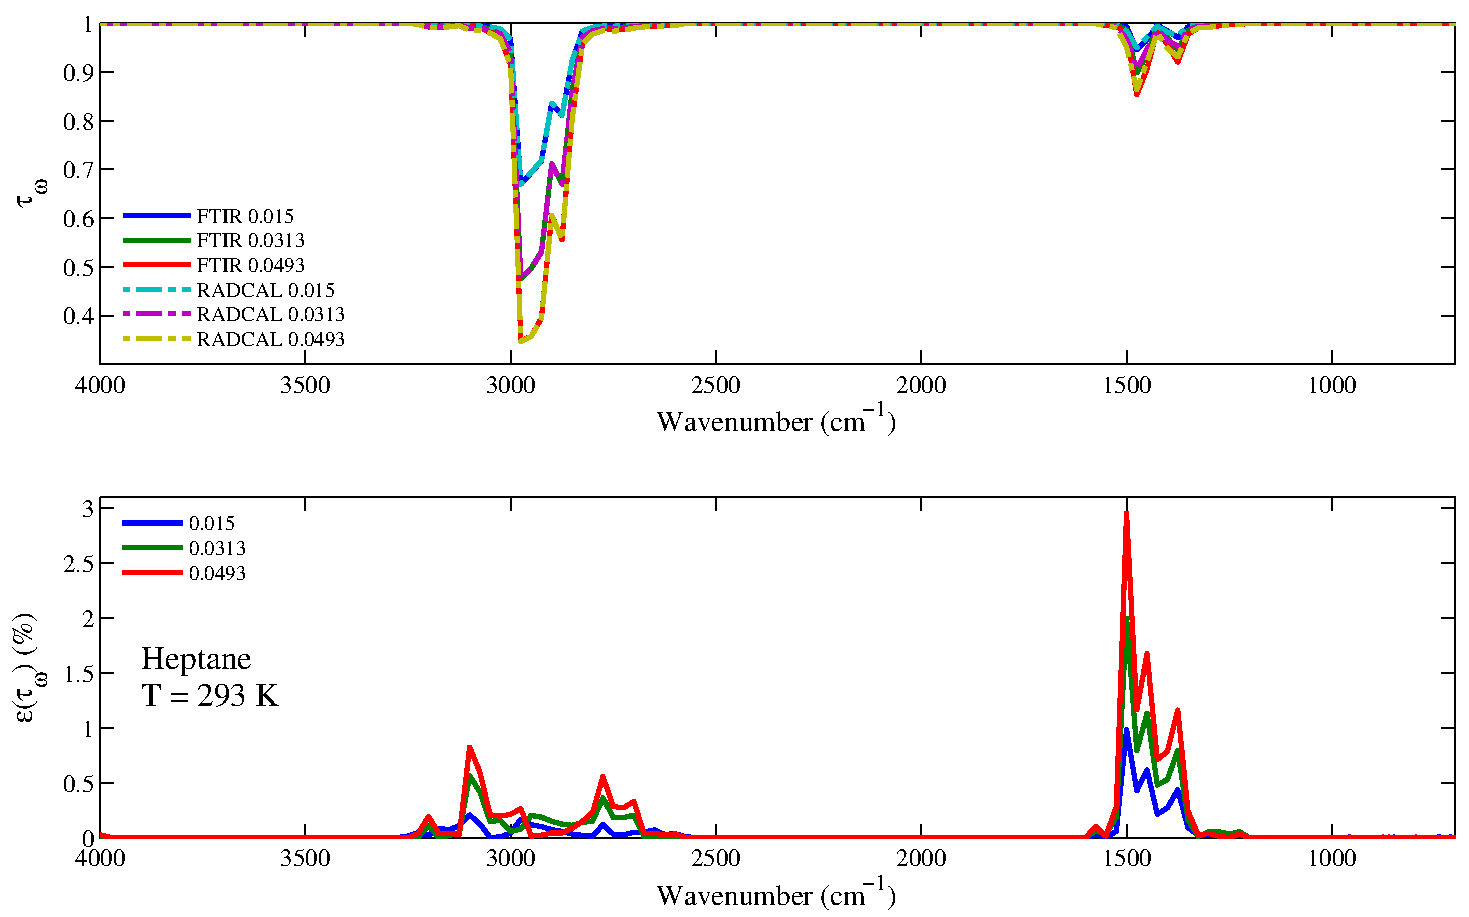
\includegraphics[width=\textwidth]{../Verification/Results_Test2/Heptane_293.pdf}
\caption{Top: comparison between the experimental (solid lines) and RadCal-generated synthetic (dashed lines) spectral transmissivity profiles, denoted $\tau_{\omega}$, of \textit{n}-heptane of an isothermal homogeneous column of \textit{n}-heptane. Bottom: relative transmissivity error, denoted $\epsilon{(\tau_{\omega})}$, between the experiment and the synthetic profiles presented on the top figure. Three different pressure path lengths are considered: 0.015, 0.0313, and 0.0493 atm.cm. The gas temperature is set at 293~K and the total pressure is 101 kPa. Note: the experimental data resolution has been changed to match that of the narrow band model. \label{fig:nheptane_Verify_293K}}
\end{figure}

\newpage

\begin{figure}[p]
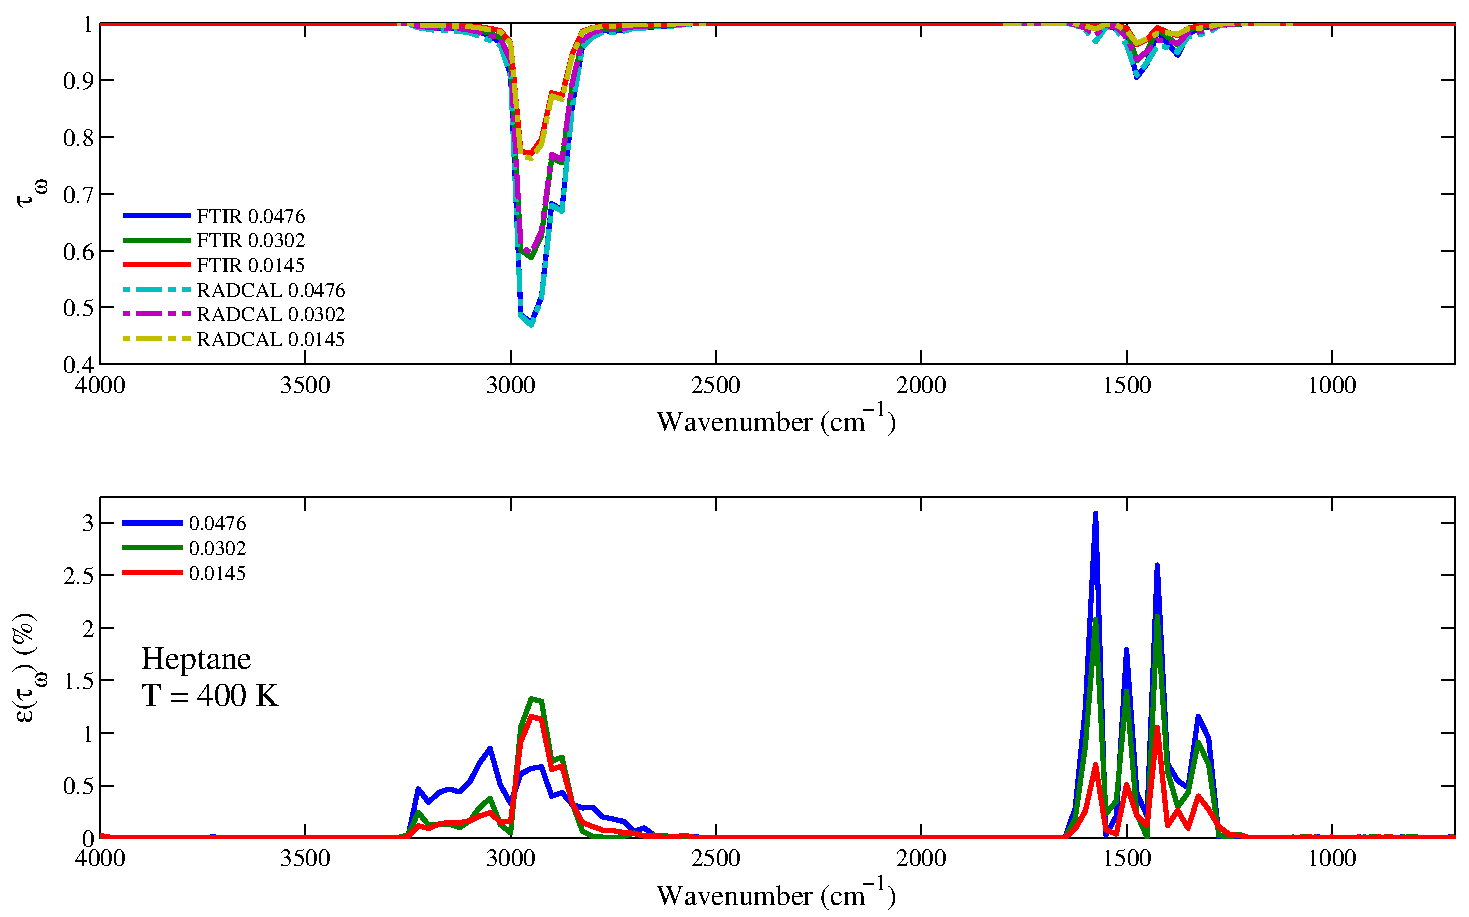
\includegraphics[width=\textwidth]{../Verification/Results_Test2/Heptane_400.pdf}
\caption{Top: comparison between the experimental (solid lines) and RadCal-generated synthetic (dashed lines) spectral transmissivity profiles, denoted $\tau_{\omega}$, of \textit{n}-heptane of an isothermal homogeneous column of \textit{n}-heptane. Bottom: relative transmissivity error, denoted $\epsilon{(\tau_{\omega})}$, between the experiment and the synthetic profiles presented on the top figure. Three different pressure path lengths are considered: 0.0476, 0.0302, and 0.0145 atm.cm. The gas temperature is set at 400~K and the total pressure is 101 kPa. Note: the experimental data resolution has been changed to match that of the narrow band model. \label{fig:nheptane_Verify_400K}}
\end{figure}

\begin{figure}[p]
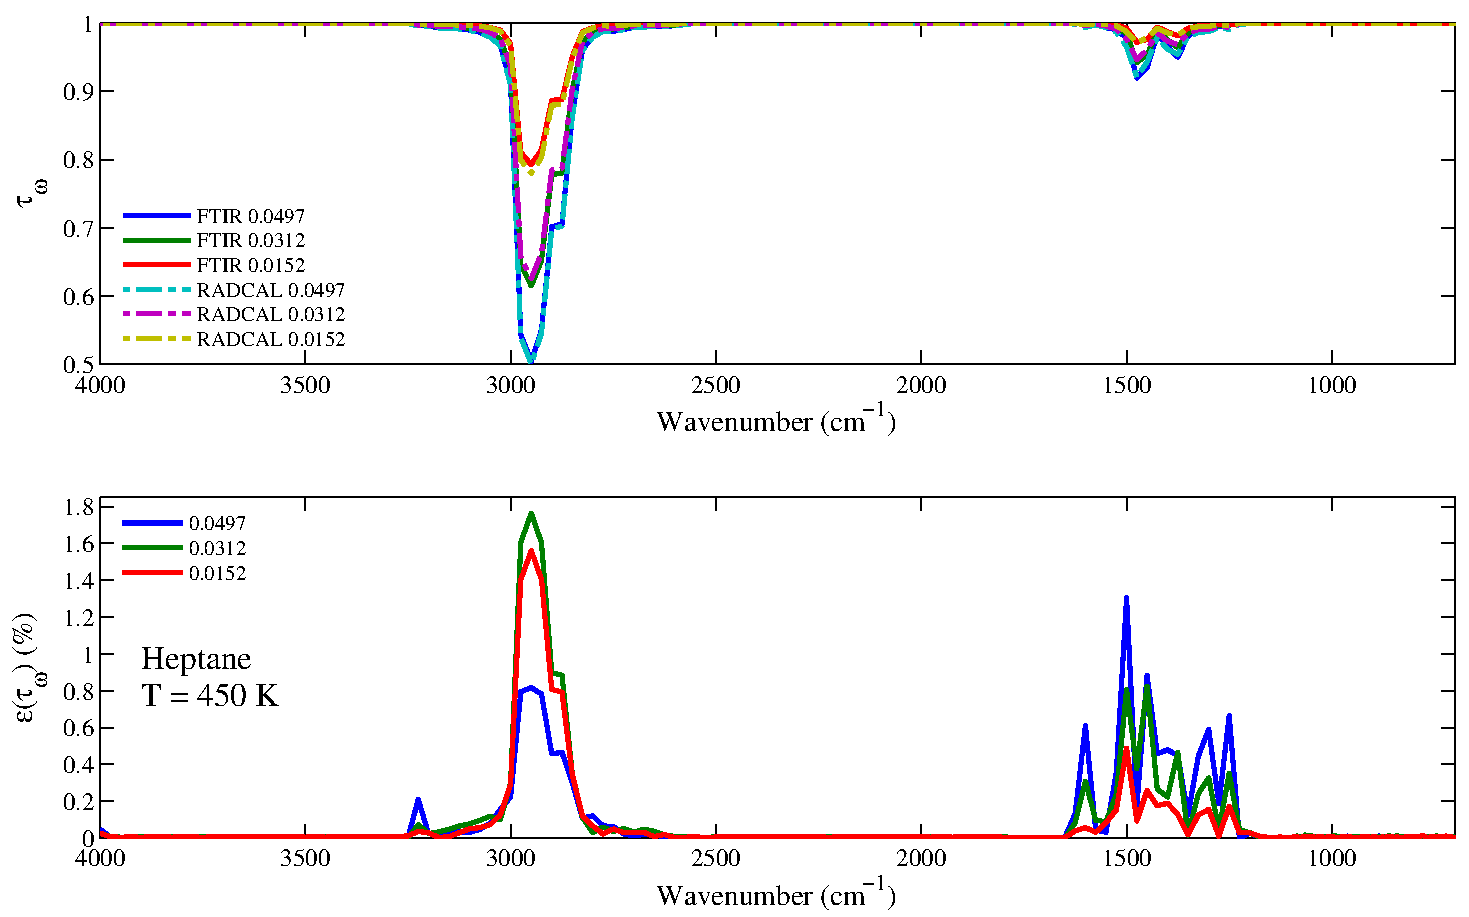
\includegraphics[width=\textwidth]{../Verification/Results_Test2/Heptane_450.pdf}
\caption{Top: comparison between the experimental (solid lines) and RadCal-generated synthetic (dashed lines) spectral transmissivity profiles, denoted $\tau_{\omega}$, of \textit{n}-heptane of an isothermal homogeneous column of \textit{n}-heptane. Bottom: relative transmissivity error, denoted $\epsilon{(\tau_{\omega})}$, between the experiment and the synthetic profiles presented on the top figure. Three different pressure path lengths are considered: 0.0497, 0.0312, and 0.0152 atm.cm. The gas temperature is set at 450~K and the total pressure is 101 kPa. Note: the experimental data resolution has been changed to match that of the narrow band model. \label{fig:nheptane_Verify_450K}}
\end{figure}

\begin{figure}[p]
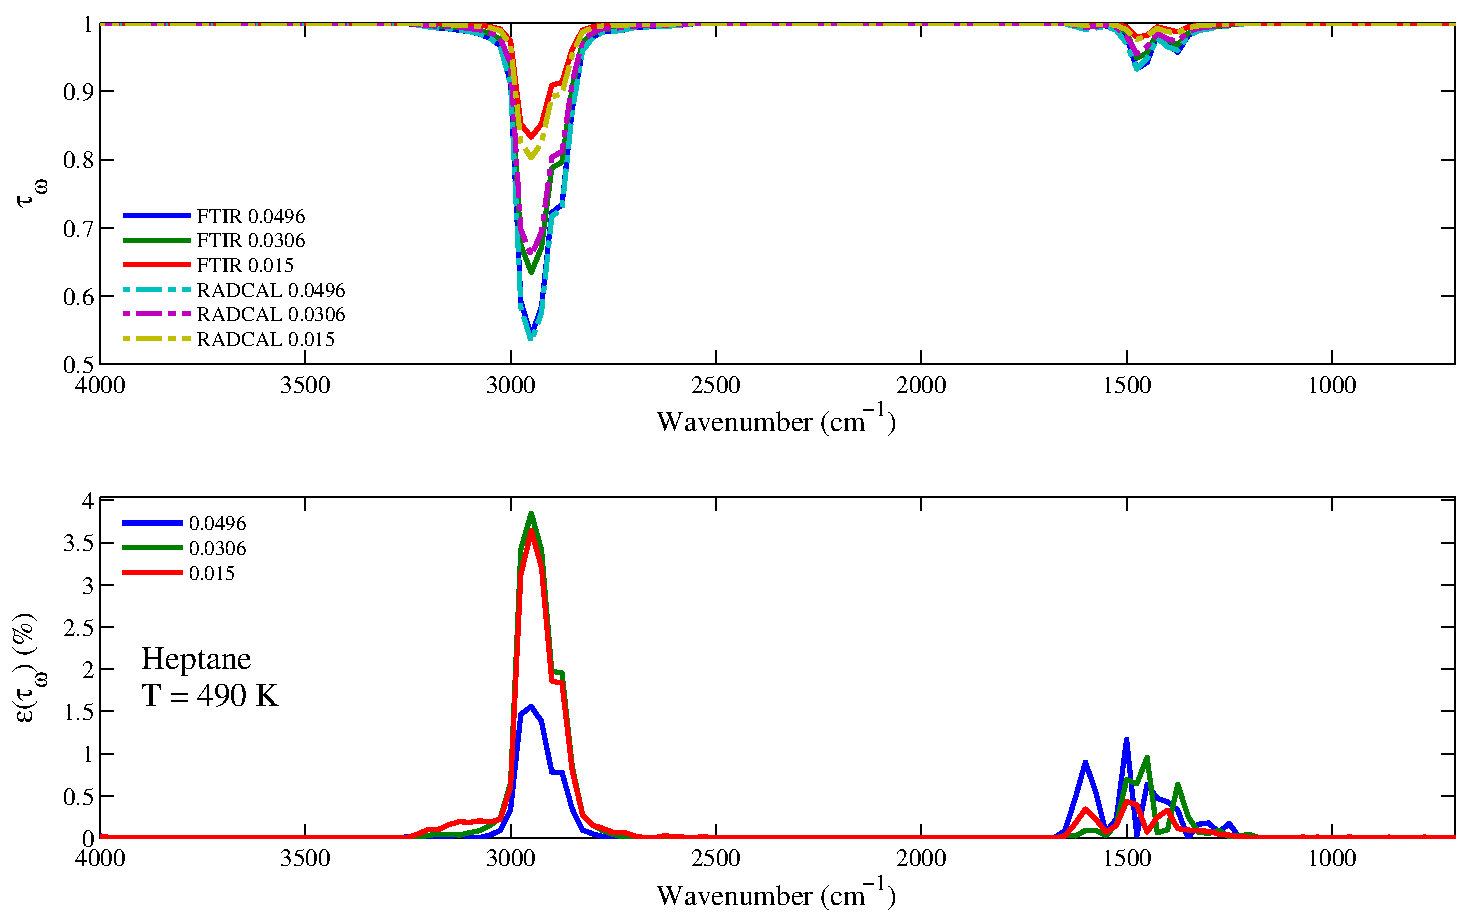
\includegraphics[width=\textwidth]{../Verification/Results_Test2/Heptane_490.pdf}
\caption{Top: comparison between the experimental (solid lines) and RadCal-generated synthetic (dashed lines) spectral transmissivity profiles, denoted $\tau_{\omega}$, of \textit{n}-heptane of an isothermal homogeneous column of \textit{n}-heptane. Bottom: relative transmissivity error, denoted $\epsilon{(\tau_{\omega})}$, between the experiment and the synthetic profiles presented on the top figure. Three different pressure path lengths are considered: 0.0496, 0.0306, and 0.015 atm.cm. The gas temperature is set at 490~K and the total pressure is 101 kPa. Note: the experimental data resolution has been changed to match that of the narrow band model. \label{fig:nheptane_Verify_490K}}
\end{figure}

\begin{figure}[p]
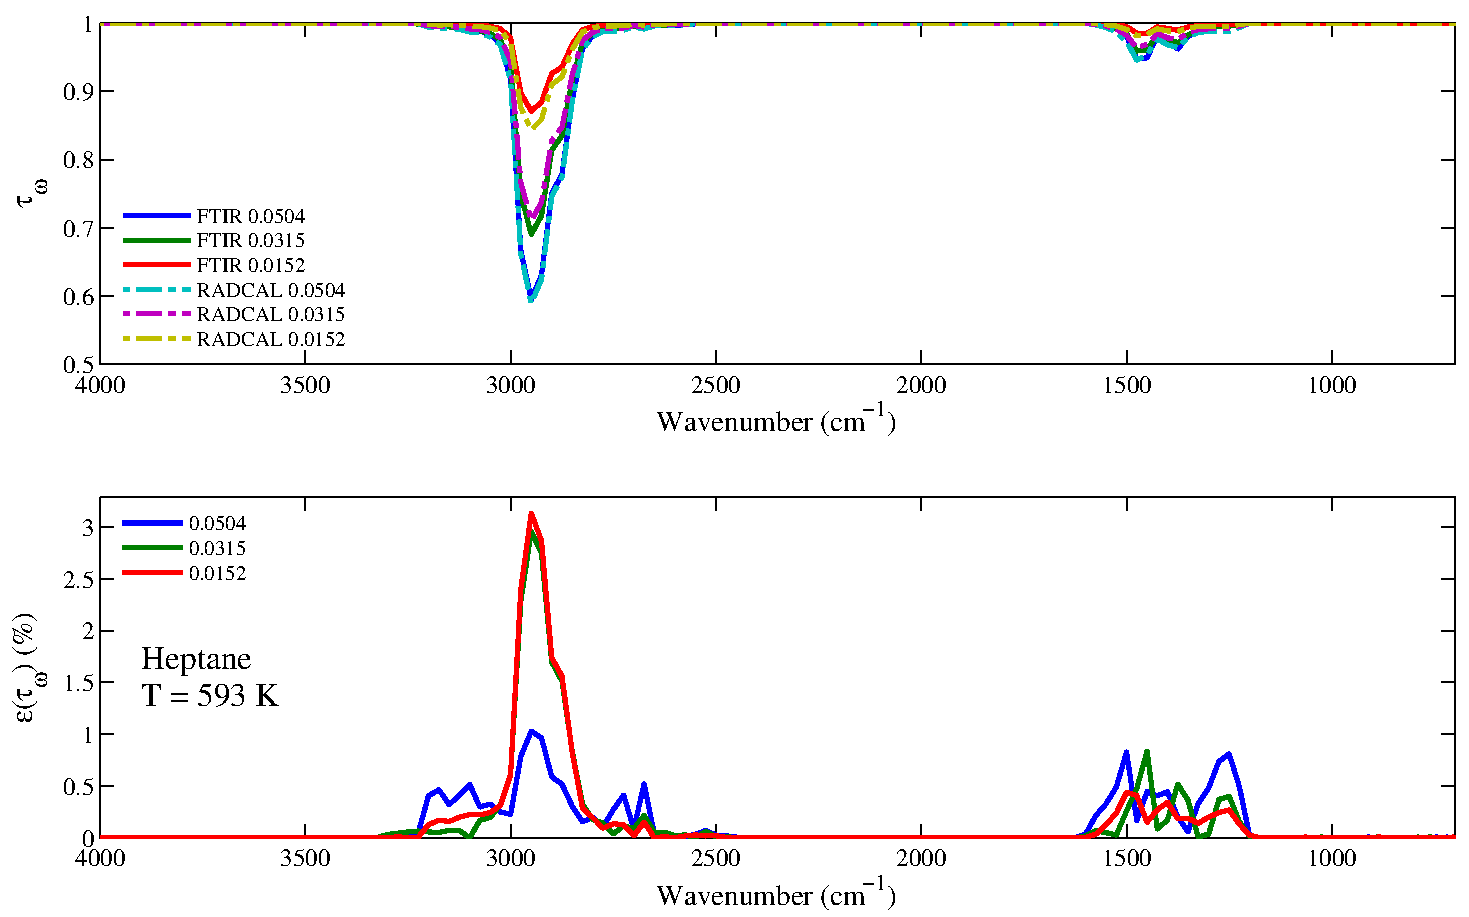
\includegraphics[width=\textwidth]{../Verification/Results_Test2/Heptane_593.pdf}
\caption{Top: comparison between the experimental (solid lines) and RadCal-generated synthetic (dashed lines) spectral transmissivity profiles, denoted $\tau_{\omega}$, of \textit{n}-heptane of an isothermal homogeneous column of \textit{n}-heptane. Bottom: relative transmissivity error, denoted $\epsilon{(\tau_{\omega})}$, between the experiment and the synthetic profiles presented on the top figure. Three different pressure path lengths are considered: 0.0504, 0.0315, and 0.0152 atm.cm. The gas temperature is set at 593~K and the total pressure is 101 kPa. Note: the experimental data resolution has been changed to match that of the narrow band model. \label{fig:nheptane_Verify_593K}}
\end{figure}

\begin{figure}[p]
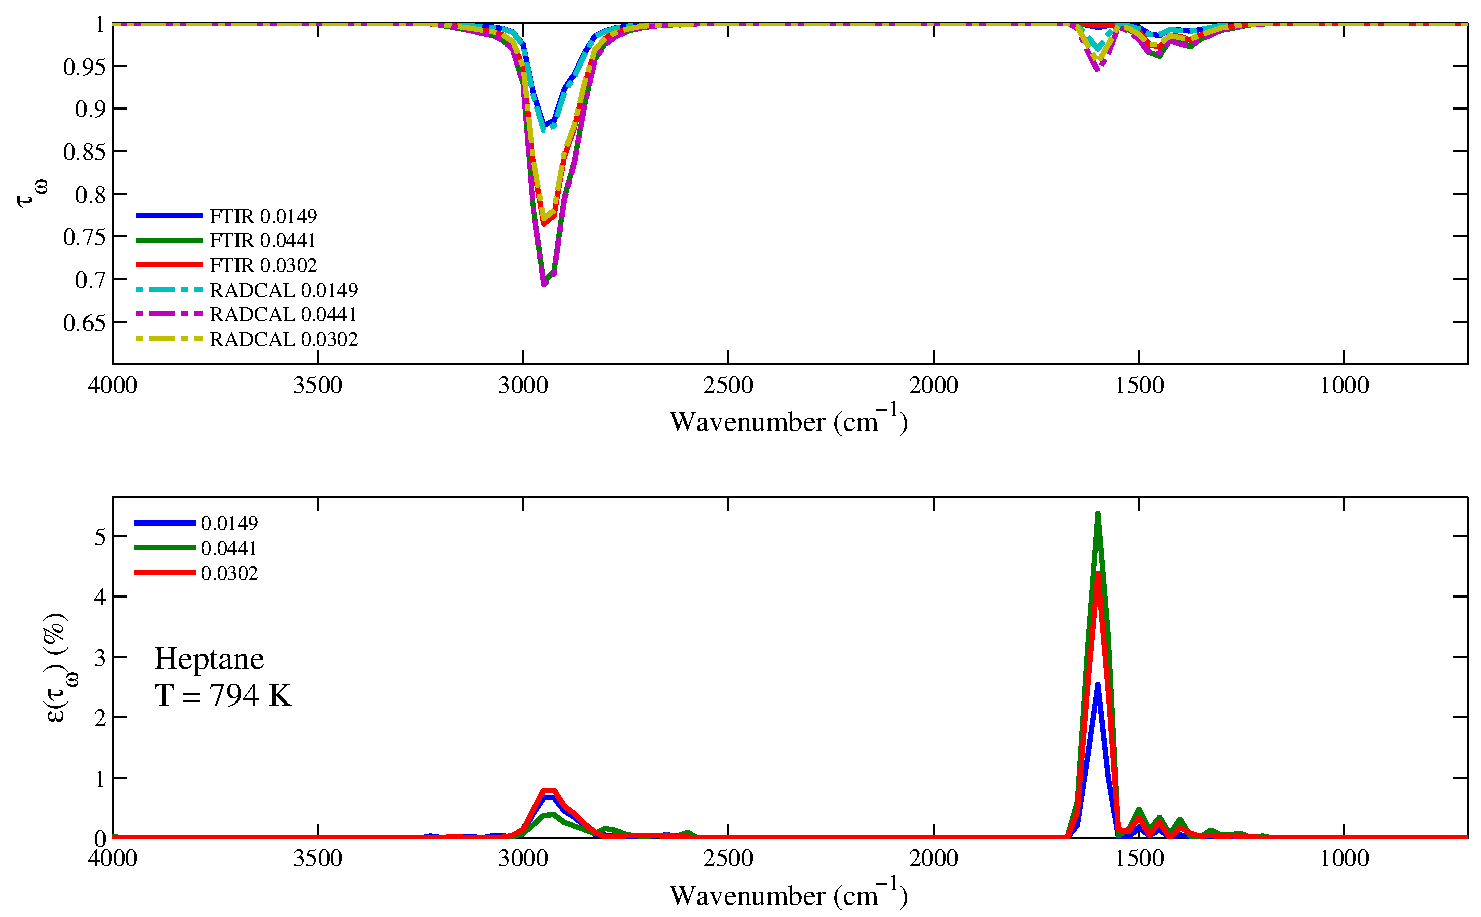
\includegraphics[width=\textwidth]{../Verification/Results_Test2/Heptane_794.pdf}
\caption{Top: comparison between the experimental (solid lines) and RadCal-generated synthetic (dashed lines) spectral transmissivity profiles, denoted $\tau_{\omega}$, of \textit{n}-heptane of an isothermal homogeneous column of \textit{n}-heptane. Bottom: relative transmissivity error, denoted $\epsilon{(\tau_{\omega})}$, between the experiment and the synthetic profiles presented on the top figure. Three different pressure path lengths are considered: 0.0149, 0.0441, and 0.0302 atm.cm. The gas temperature is set at 794~K and the total pressure is 101 kPa. Note: the experimental data resolution has been changed to match that of the narrow band model. \label{fig:nheptane_Verify_794K}}
\end{figure}

\begin{figure}[p]
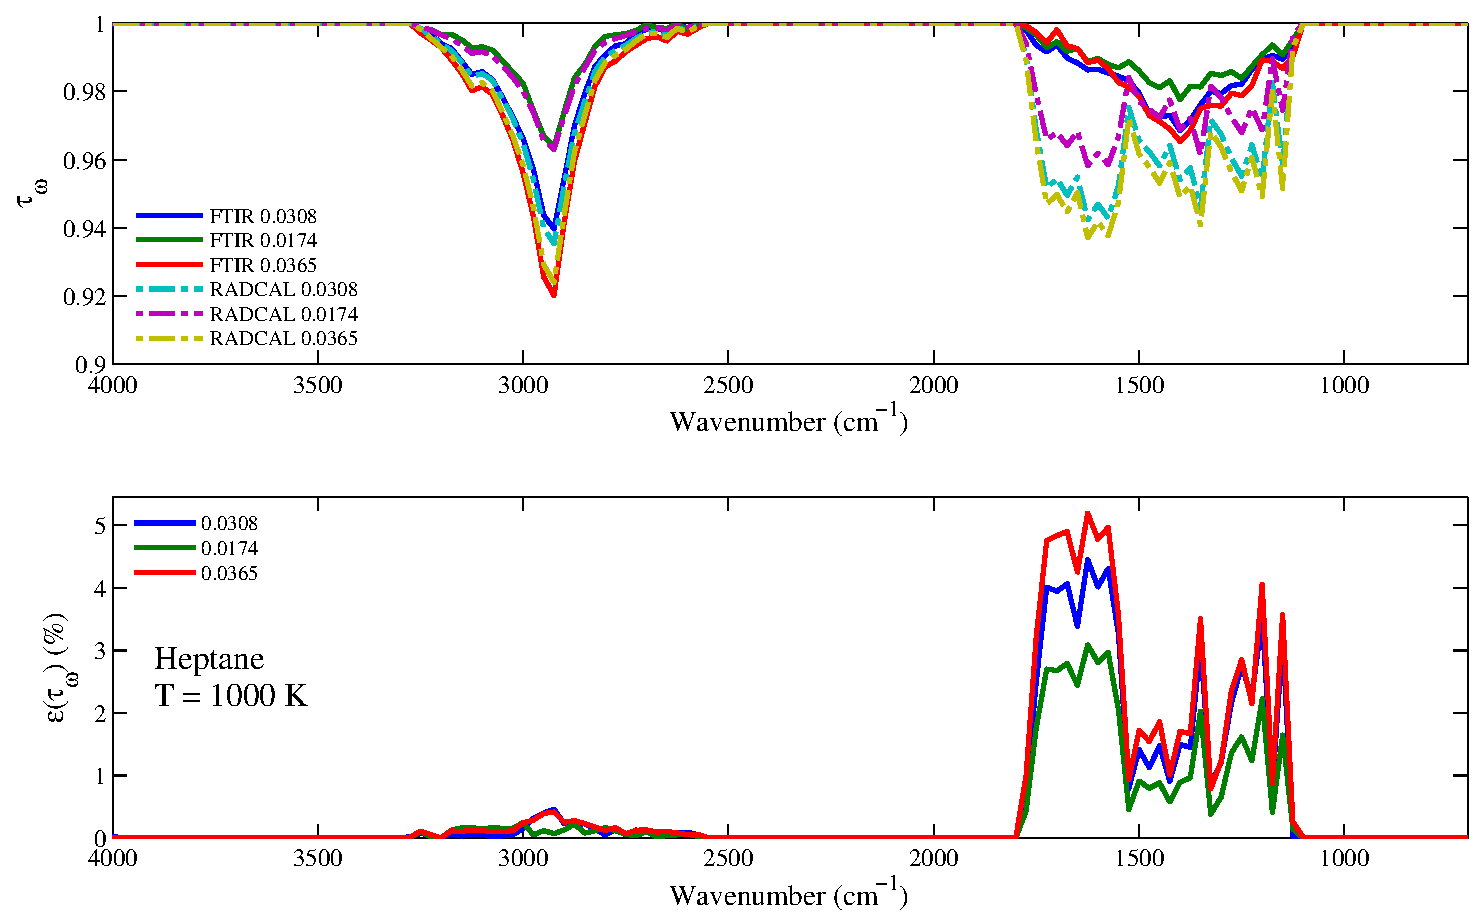
\includegraphics[width=\textwidth]{../Verification/Results_Test2/Heptane_1000.pdf}
\caption{Top: comparison between the experimental (solid lines) and RadCal-generated synthetic (dashed lines) spectral transmissivity profiles, denoted $\tau_{\omega}$, of \textit{n}-heptane of an isothermal homogeneous column of \textit{n}-heptane. Bottom: relative transmissivity error, denoted $\epsilon{(\tau_{\omega})}$, between the experiment and the synthetic profiles presented on the top figure. Three different pressure path lengths are considered: 0.0308, 0.0174, and 0.0365 atm.cm. The gas temperature is set at 1000~K and the total pressure is 101 kPa. Note: the experimental data resolution has been changed to match that of the narrow band model. \label{fig:nheptane_Verify_1000K}}
\end{figure}


\clearpage

\section{Methanol: $\rm CH_3OH$}

\begin{figure}[h]
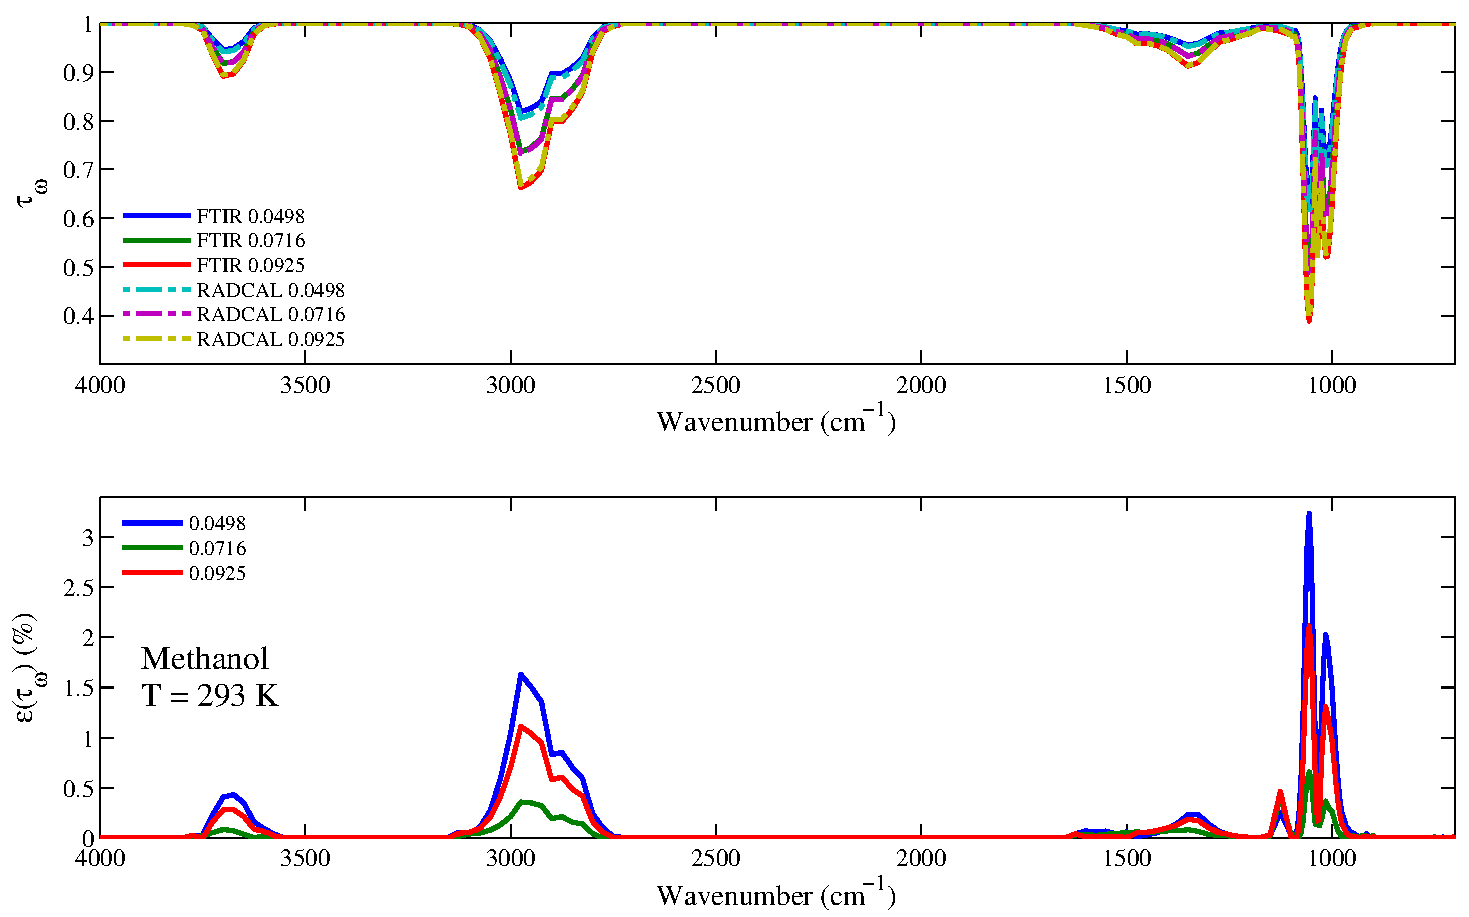
\includegraphics[width=\textwidth]{../Verification/Results_Test2/Methanol_293.pdf}
\caption{Top: comparison between the experimental (solid lines) and RadCal-generated synthetic (dashed lines) spectral transmissivity profiles, denoted $\tau_{\omega}$, of methanol of an isothermal homogeneous column of methanol. Bottom: relative transmissivity error, denoted $\epsilon{(\tau_{\omega})}$, between the experiment and the synthetic profiles presented on the top figure. Three different pressure path lengths are considered: 0.0498, 0.0716, and 0.0925 atm.cm. The gas temperature is set at 293~K and the total pressure is 101 kPa. Note: the experimental data resolution has been changed to match that of the narrow band model. \label{fig:methanol_Verify_293K}}
\end{figure}

\newpage

\begin{figure}[p]
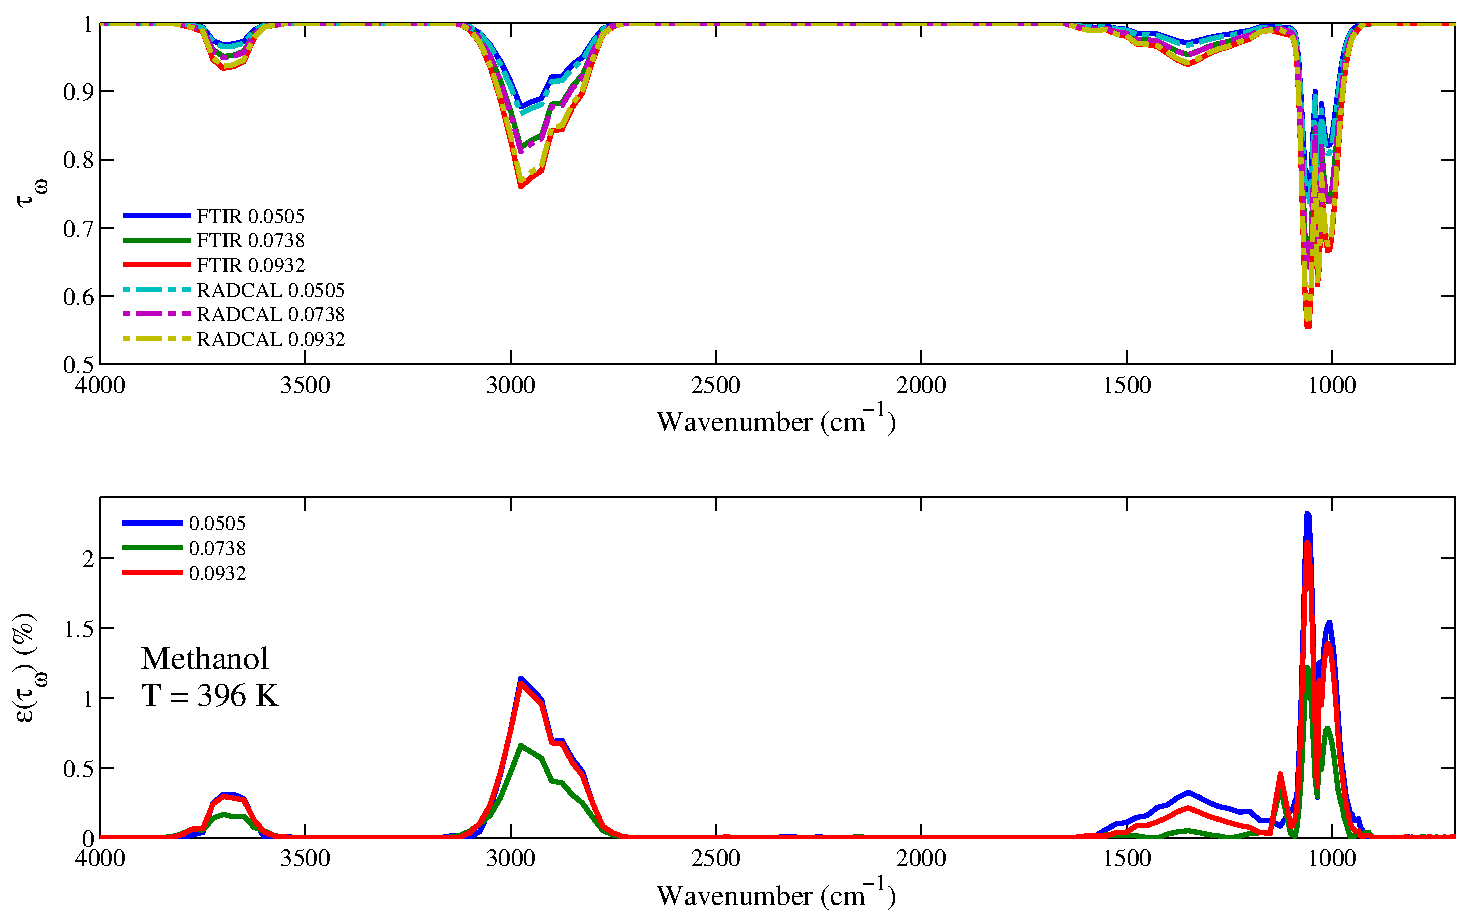
\includegraphics[width=\textwidth]{../Verification/Results_Test2/Methanol_396.pdf}
\caption{Top: comparison between the experimental (solid lines) and RadCal-generated synthetic (dashed lines) spectral transmissivity profiles, denoted $\tau_{\omega}$, of methanol of an isothermal homogeneous column of methanol. Bottom: relative transmissivity error, denoted $\epsilon{(\tau_{\omega})}$, between the experiment and the synthetic profiles presented on the top figure. Three different pressure path lengths are considered: 0.0505, 0.0738, and 0.0932 atm.cm. The gas temperature is set at 396~K and the total pressure is 101 kPa. Note: the experimental data resolution has been changed to match that of the narrow band model. \label{fig:methanol_Verify_396K}}
\end{figure}

\begin{figure}[p]
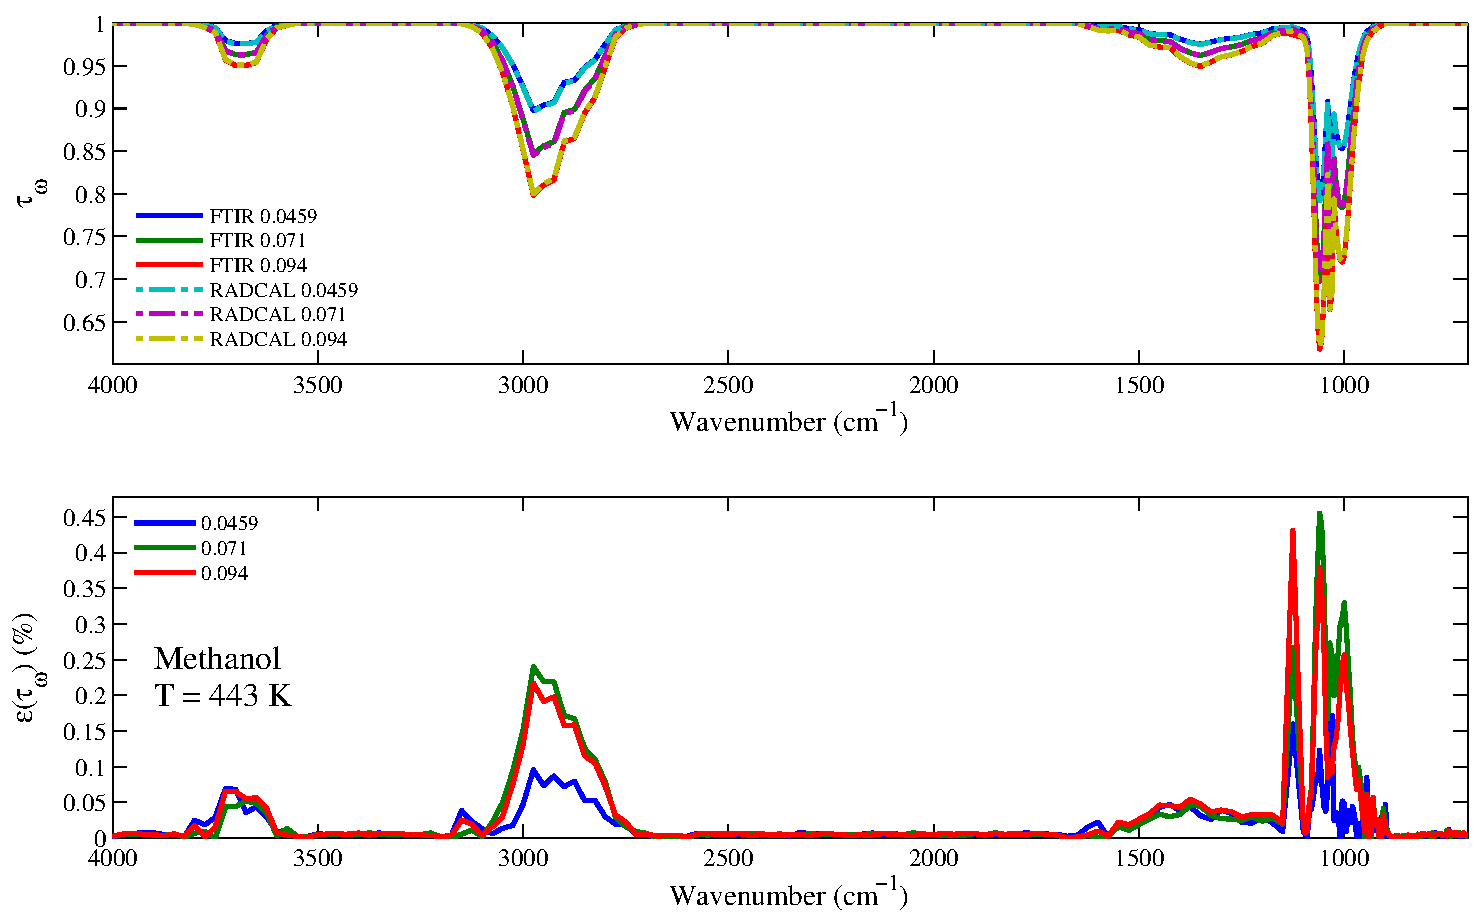
\includegraphics[width=\textwidth]{../Verification/Results_Test2/Methanol_443.pdf}
\caption{Top: comparison between the experimental (solid lines) and RadCal-generated synthetic (dashed lines) spectral transmissivity profiles, denoted $\tau_{\omega}$, of methanol of an isothermal homogeneous column of methanol. Bottom: relative transmissivity error, denoted $\epsilon{(\tau_{\omega})}$, between the experiment and the synthetic profiles presented on the top figure. Three different pressure path lengths are considered: 0.0459, 0.071, and 0.094 atm.cm. The gas temperature is set at 443~K and the total pressure is 101 kPa. Note: the experimental data resolution has been changed to match that of the narrow band model. \label{fig:methanol_Verify_443K}}
\end{figure}

\begin{figure}[p]
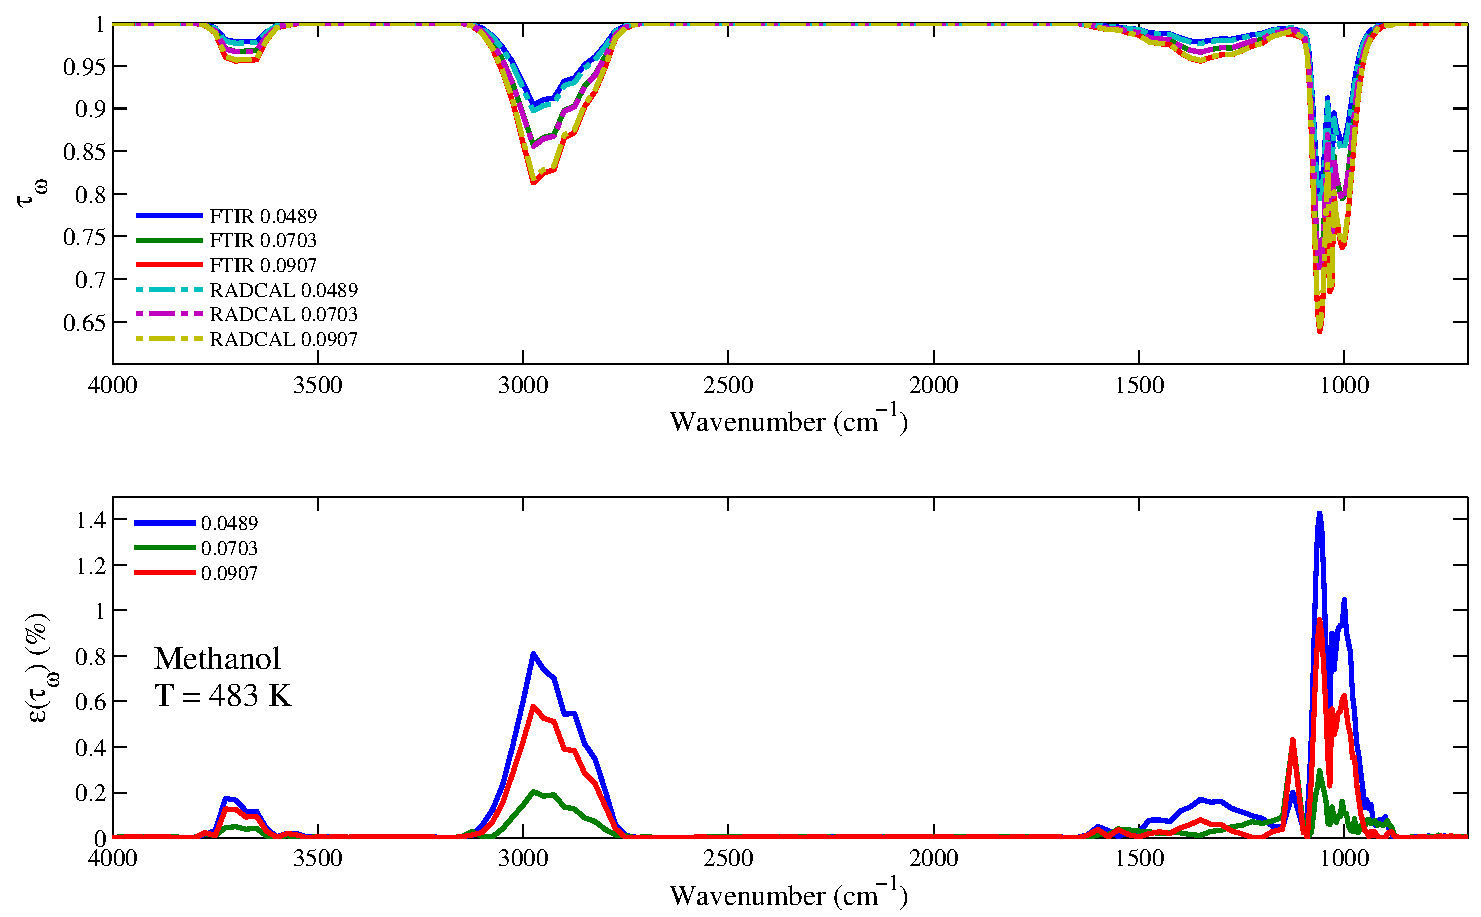
\includegraphics[width=\textwidth]{../Verification/Results_Test2/Methanol_483.pdf}
\caption{Top: comparison between the experimental (solid lines) and RadCal-generated synthetic (dashed lines) spectral transmissivity profiles, denoted $\tau_{\omega}$, of methanol of an isothermal homogeneous column of methanol. Bottom: relative transmissivity error, denoted $\epsilon{(\tau_{\omega})}$, between the experiment and the synthetic profiles presented on the top figure. Three different pressure path lengths are considered: 0.0489, 0.0703, and 0.0907 atm.cm. The gas temperature is set at 483~K and the total pressure is 101 kPa. Note: the experimental data resolution has been changed to match that of the narrow band model. \label{fig:methanol_Verify_483K}}
\end{figure}

\begin{figure}[p]
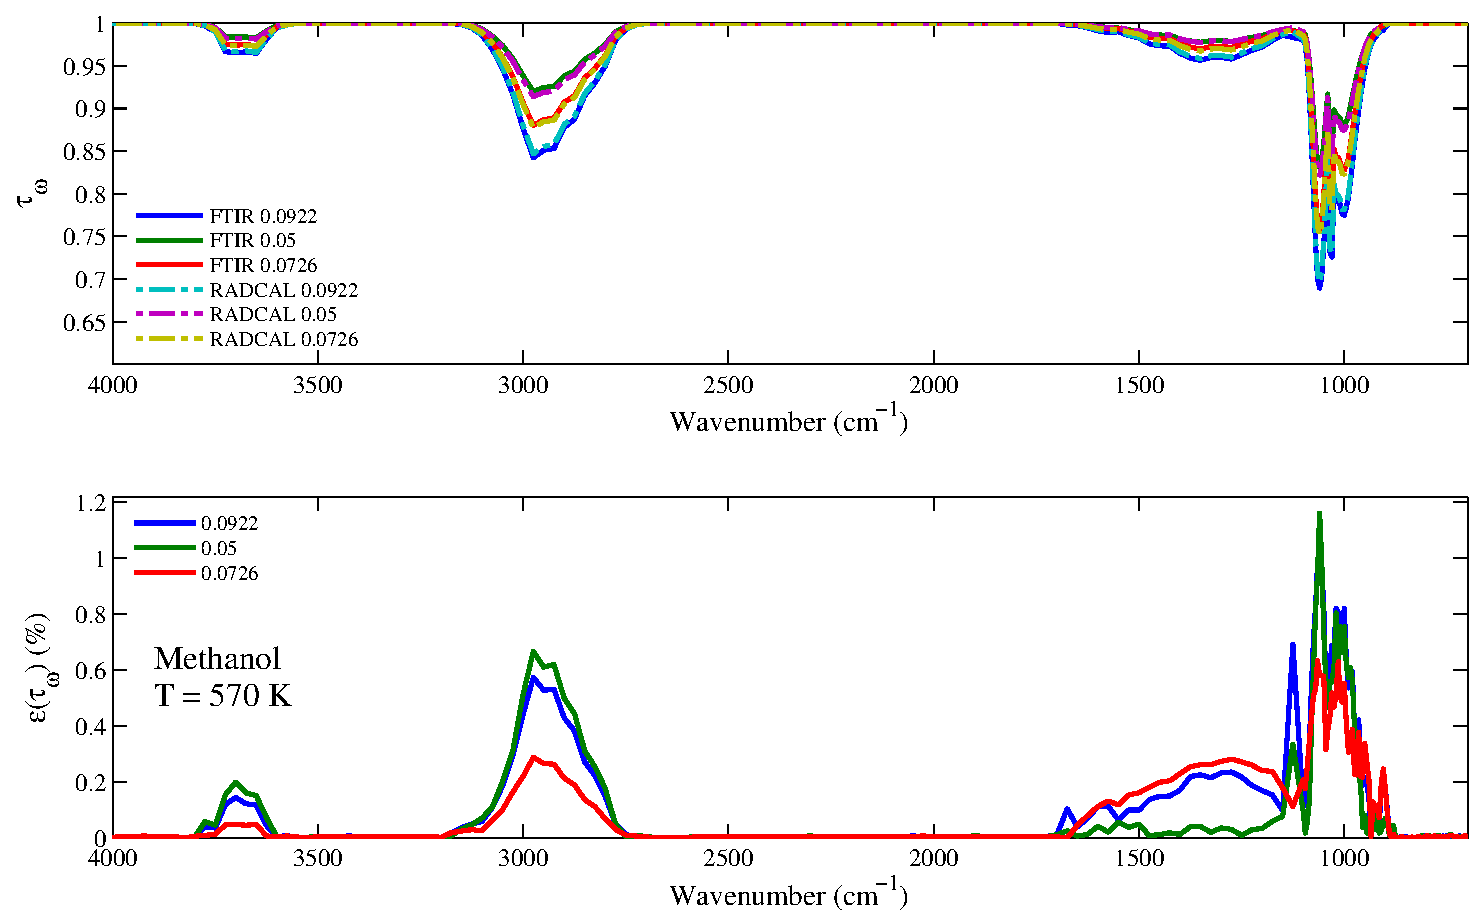
\includegraphics[width=\textwidth]{../Verification/Results_Test2/Methanol_570.pdf}
\caption{Top: comparison between the experimental (solid lines) and RadCal-generated synthetic (dashed lines) spectral transmissivity profiles, denoted $\tau_{\omega}$, of methanol of an isothermal homogeneous column of methanol. Bottom: relative transmissivity error, denoted $\epsilon{(\tau_{\omega})}$, between the experiment and the synthetic profiles presented on the top figure. Three different pressure path lengths are considered: 0.0922, 0.05, and 0.0726 atm.cm. The gas temperature is set at 570~K and the total pressure is 101 kPa. Note: the experimental data resolution has been changed to match that of the narrow band model. \label{fig:methanol_Verify_570K}}
\end{figure}

\begin{figure}[p]
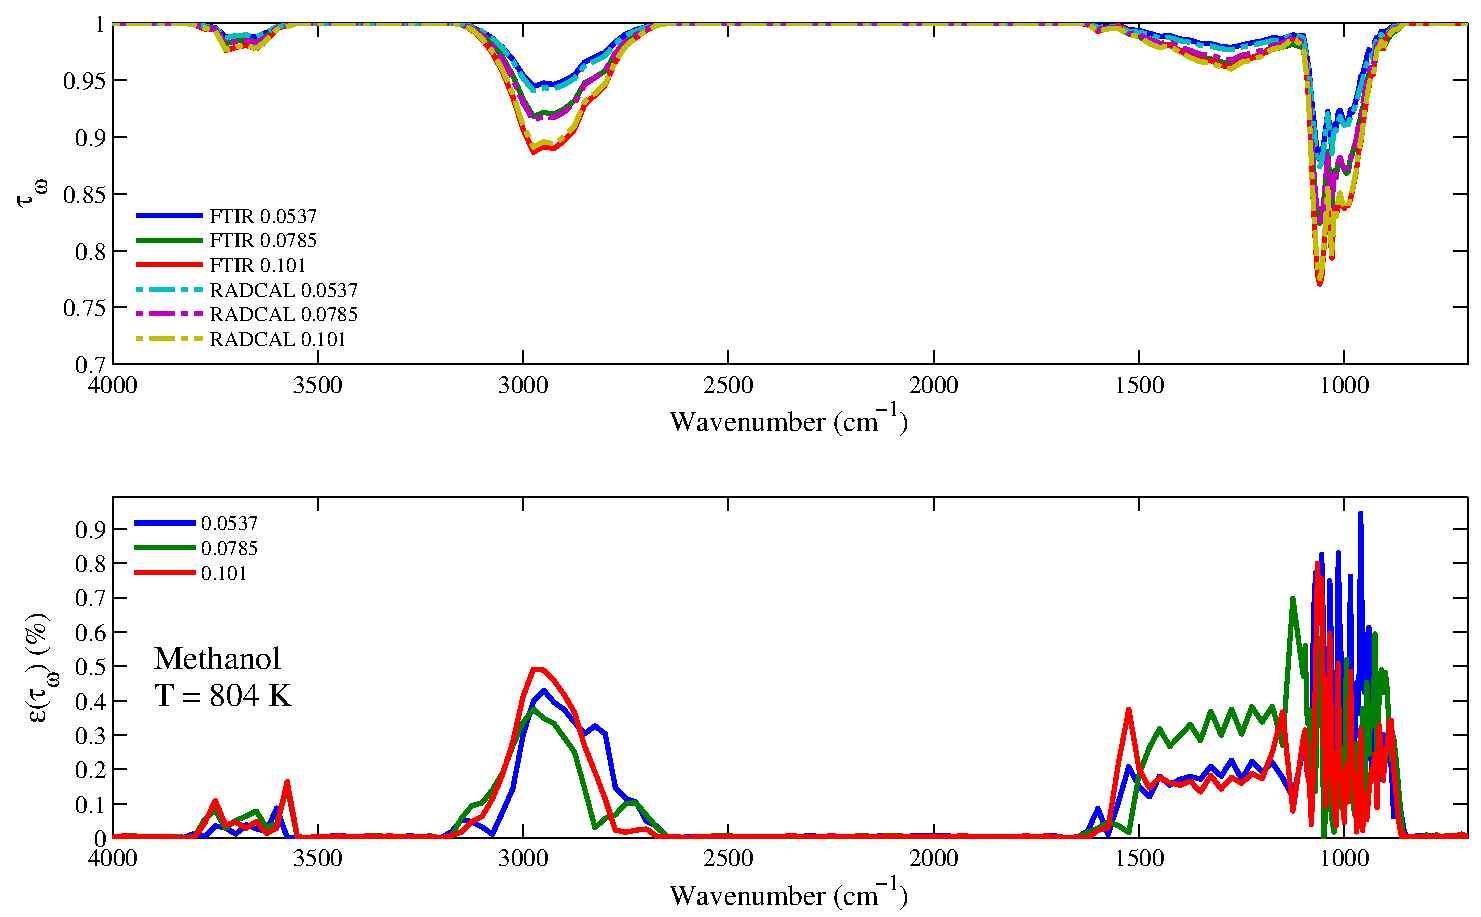
\includegraphics[width=\textwidth]{../Verification/Results_Test2/Methanol_804.pdf}
\caption{Top: comparison between the experimental (solid lines) and RadCal-generated synthetic (dashed lines) spectral transmissivity profiles, denoted $\tau_{\omega}$, of methanol of an isothermal homogeneous column of methanol. Bottom: relative transmissivity error, denoted $\epsilon{(\tau_{\omega})}$, between the experiment and the synthetic profiles presented on the top figure. Three different pressure path lengths are considered: 0.0537, 0.0785, and 0.101 atm.cm. The gas temperature is set at 804~K and the total pressure is 101 kPa. Note: the experimental data resolution has been changed to match that of the narrow band model. \label{fig:methanol_Verify_804K}}
\end{figure}

\begin{figure}[p]
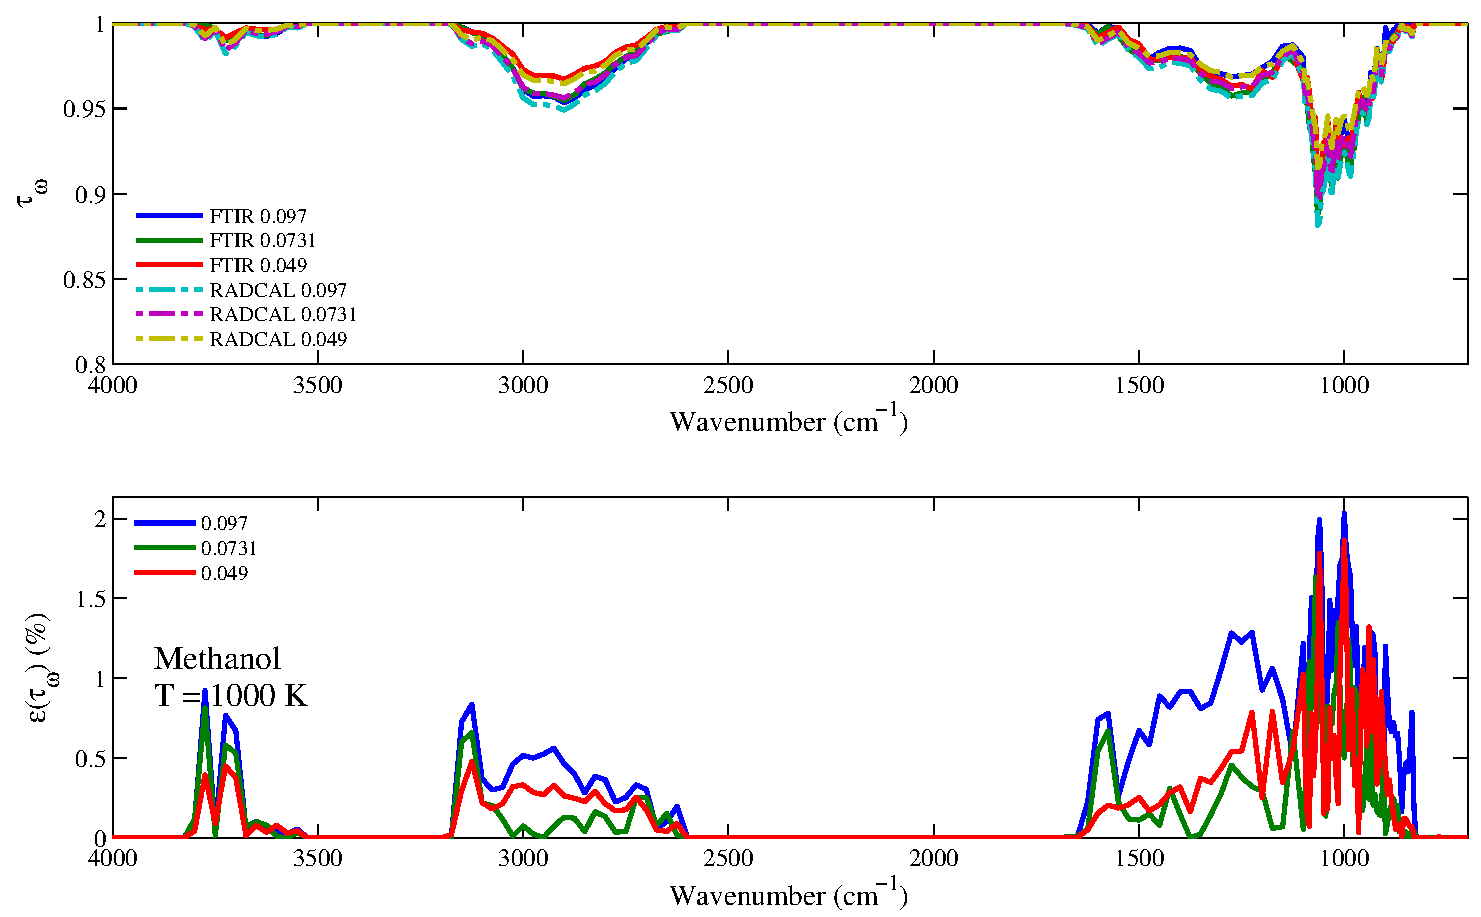
\includegraphics[width=\textwidth]{../Verification/Results_Test2/Methanol_1000.pdf}
\caption{Top: comparison between the experimental (solid lines) and RadCal-generated synthetic (dashed lines) spectral transmissivity profiles, denoted $\tau_{\omega}$, of methanol of an isothermal homogeneous column of methanol. Bottom: relative transmissivity error, denoted $\epsilon{(\tau_{\omega})}$, between the experiment and the synthetic profiles presented on the top figure. Three different pressure path lengths are considered: 0.097, 0.0731, and 0.049 atm.cm. The gas temperature is set at 1000~K and the total pressure is 101 kPa. Note: the experimental data resolution has been changed to match that of the narrow band model. \label{fig:methanol_Verify_1000K}}
\end{figure}


\clearpage

\section{Methyl Methacrylate: $\rm C_5H_8O_2$}

\begin{figure}[h]
\includegraphics[width=\textwidth]{../Verification/Results_Test2/MMA_297.pdf}
\caption{Top: comparison between the experimental (solid lines) and RadCal-generated synthetic (dashed lines) spectral transmissivity profiles, denoted $\tau_{\omega}$, of MMA of an isothermal homogeneous column of MMA. Bottom: relative transmissivity error, denoted $\epsilon{(\tau_{\omega})}$, between the experiment and the synthetic profiles presented on the top figure. Three different pressure path lengths are considered: 0.1, 0.0785, and 0.0545 atm.cm. The gas temperature is set at 297~K and the total pressure is 101 kPa. Note: the experimental data resolution has been changed to match that of the narrow band model. \label{fig:MMA_Verify_297K}}
\end{figure}

\newpage

\begin{figure}[p]
\includegraphics[width=\textwidth]{../Verification/Results_Test2/MMA_396.pdf}
\caption{Top: comparison between the experimental (solid lines) and RadCal-generated synthetic (dashed lines) spectral transmissivity profiles, denoted $\tau_{\omega}$, of MMA of an isothermal homogeneous column of MMA. Bottom: relative transmissivity error, denoted $\epsilon{(\tau_{\omega})}$, between the experiment and the synthetic profiles presented on the top figure. Three different pressure path lengths are considered: 0.102, 0.179, and 0.0782 atm.cm. The gas temperature is set at 396~K and the total pressure is 101 kPa. Note: the experimental data resolution has been changed to match that of the narrow band model. \label{fig:MMA_Verify_396K}}
\end{figure}

\begin{figure}[p]
\includegraphics[width=\textwidth]{../Verification/Results_Test2/MMA_441.pdf}
\caption{Top: comparison between the experimental (solid lines) and RadCal-generated synthetic (dashed lines) spectral transmissivity profiles, denoted $\tau_{\omega}$, of MMA of an isothermal homogeneous column of MMA. Bottom: relative transmissivity error, denoted $\epsilon{(\tau_{\omega})}$, between the experiment and the synthetic profiles presented on the top figure. Three different pressure path lengths are considered: 0.0946, 0.074, and 0.0508 atm.cm. The gas temperature is set at 441~K and the total pressure is 101 kPa. Note: the experimental data resolution has been changed to match that of the narrow band model. \label{fig:MMA_Verify_443K}}
\end{figure}

\begin{figure}[p]
\includegraphics[width=\textwidth]{../Verification/Results_Test2/MMA_483.pdf}
\caption{Top: comparison between the experimental (solid lines) and RadCal-generated synthetic (dashed lines) spectral transmissivity profiles, denoted $\tau_{\omega}$, of MMA of an isothermal homogeneous column of MMA. Bottom: relative transmissivity error, denoted $\epsilon{(\tau_{\omega})}$, between the experiment and the synthetic profiles presented on the top figure. Three different pressure path lengths are considered: 0.0956, 0.0742, and 0.0512 atm.cm. The gas temperature is set at 483~K and the total pressure is 101 kPa. Note: the experimental data resolution has been changed to match that of the narrow band model. \label{fig:MMA_Verify_483K}}
\end{figure}

\begin{figure}[p]
\includegraphics[width=\textwidth]{../Verification/Results_Test2/MMA_597.pdf}
\caption{Top: comparison between the experimental (solid lines) and RadCal-generated synthetic (dashed lines) spectral transmissivity profiles, denoted $\tau_{\omega}$, of MMA of an isothermal homogeneous column of MMA. Bottom: relative transmissivity error, denoted $\epsilon{(\tau_{\omega})}$, between the experiment and the synthetic profiles presented on the top figure. Three different pressure path lengths are considered: 0.0966, 0.0746, and 0.0516 atm.cm. The gas temperature is set at 597~K and the total pressure is 101 kPa. Note: the experimental data resolution has been changed to match that of the narrow band model. \label{fig:MMA_Verify_597K}}
\end{figure}

\begin{figure}[p]
\includegraphics[width=\textwidth]{../Verification/Results_Test2/MMA_803.pdf}
\caption{Top: comparison between the experimental (solid lines) and RadCal-generated synthetic (dashed lines) spectral transmissivity profiles, denoted $\tau_{\omega}$, of MMA of an isothermal homogeneous column of MMA. Bottom: relative transmissivity error, denoted $\epsilon{(\tau_{\omega})}$, between the experiment and the synthetic profiles presented on the top figure. Three different pressure path lengths are considered: 0.106, 0.081, and 0.0554 atm.cm. The gas temperature is set at 803~K and the total pressure is 101 kPa. Note: the experimental data resolution has been changed to match that of the narrow band model. \label{fig:MMA_Verify_803K}}
\end{figure}

\begin{figure}[p]
\includegraphics[width=\textwidth]{../Verification/Results_Test2/MMA_1014.pdf}
\caption{Top: comparison between the experimental (solid lines) and RadCal-generated synthetic (dashed lines) spectral transmissivity profiles, denoted $\tau_{\omega}$, of MMA of an isothermal homogeneous column of MMA. Bottom: relative transmissivity error, denoted $\epsilon{(\tau_{\omega})}$, between the experiment and the synthetic profiles presented on the top figure. Three different pressure path lengths are considered: 0.114, 0.0879, and 0.0598 atm.cm. The gas temperature is set at 1014~K and the total pressure is 101 kPa. Note: the experimental data resolution has been changed to match that of the narrow band model. \label{fig:MMA_Verify_1014K}}
\end{figure}
